\chapter{High Voltage}
\label{ch:dp-hv}


%%%%%%%%%%%%%%%%%%%%%%%%%%%%%%%%%%%%%%%%%%%%%%%%%%%%%%%%%%%%%%%%%%%%
%\section{High Voltage System Overview}
\label{sec:fddp-hv-ov}

%%%%%%%%%%%%%%%%%%%%%%%%%%%%
%\subsection{Introduction - 2 pages}
\label{sec:fddp-hv-intro}

A \dword{lartpc} requires an equipotential cathode plane at \dword{hv} and a precisely regulated interior \efield to drive the
electrons from particle interactions to the sensor planes. For the \dword{dune} %\dlong{dp} (\dword{dp}) 
\dword{dp} technology, 
this requires a horizontal cathode plane, held at a negative \dword{hv}; a horizontal \dword{crp} in the gas phase as described in Chapter~\ref{sec:fddp-crp-intro}; %and formed sets of conductors at graded voltages surrounding the the central drift volume, collectively called the \dword{fc}, shown in Figure~\ref{fig:dune_dp_fd_hvs}. The \dword{fc} consists of electrically and mechanically continuous field shaping rings that provide voltage degradation in the vertical direction and forms one continuous active volume. (Anne edited)
and electrically and mechanically continuous horizontal field-shaping rings that surround the central active drift volume, providing a linear voltage gradient in the vertical direction, collectively called the \dword{fc}. The \dual \dword{hv} system components are shown in Figure~\ref{fig:dune_dp_fd_hvs}.
%, shown in Figure~\ref{fig:dune_dp_fd_hvs}.

\begin{dunefigure}[DUNE \dual detector module  overview]{fig:dune_dp_fd_hvs}
{An isometric view of the \dword{dp} \dword{hv} system components. Most of the \dword{fc} profiles are removed to emphasize the structural elements.  The figure shows three completed \dword{fc} super-modules, described in detail in Section~\ref{sec:dp-hv-system-fc}; cathode planes attached to the bottom of the three super-modules on the upper right; the structural members of the \dword{fc} and cathode plane in the lower left; and half the ground grid modules on the bottom. The entire structure, other than the ground grid that lies on the floor, is suspended on stainless steel I-beams under the cryostat ceiling by 24 cables and rods (Credit: BNL) }.
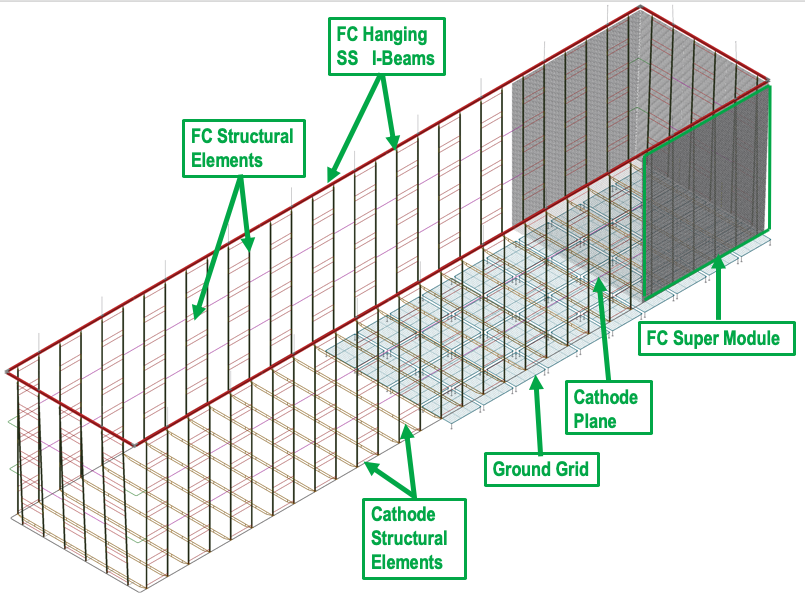
\includegraphics[width=0.9\textwidth]{graphics/DP_HVS_v2.png}
\end{dunefigure}

%\fixme{need to define super-module and module. If a super-module is a set of three stacks of six sub-modules each, is a stack then a 'module'? We go from super to sub module. Anne} --- defined later

The \dword{hv} consortium will provide a system that operates at the nominal voltage corresponding to the uniform \SI{500}{V/cm} \efield in the \dword{tpc} drift volume. 
%As a result, its systems %actually constitute a large fraction of the %total internal structures of the \dword{tpc}. % itself. 
Mechanical and structural concerns are taken into account, as well as the electrical design to meet the requirements. 

%%%%%%%%%%%%%%%%%%%%%%%%%%%%
\section{Scope}
\label{sec:fddp-hv-scope}
The scope of the \dual \dword{hv} system, provided by the \dword{dune} \dword{hv} consortium includes selecting and procuring materials, as well as fabricating, testing, delivering, and installing the components needed to generate, distribute, and regulate the voltages that create a stable and precise \efield{} within the \dune \dword{dpmod}. 

The \dual \dword{hv} system has the following components:

\begin{itemize}
\item \SI{-600}{kV} \dword{hvps}, cable, filters, and \fdth;
\item \dword{hv} extender and voltage degrader;
\item horizontal cathode plane (\SI{60}{\m} long and \SI{12}{\m} wide) made of arrays of resistive elements placed approximately \SI{1.5}{\m} above the bottom of the cryostat;
\item \dwords{gp} below the cathode to protect the \dword{pd} array;
\item vertical \dword{fc} walls, \SI{12}{\m} tall surrounding the cathode and covering a total of \SI{144}{\m} circumference; and
\item \dword{hv} return \fdth and resistor box.
\end{itemize}

The \dword{hv} system consists of components both exterior and interior to the cryostat. The \dword{hvps} is external, mounted on top of the \dword{hv} \fdth, eliminating the need for %a thick dielectric layer on 
 the external \dword{hv} cable. 
%\fixme{do we have a HV cable and filter in this design?}
%The voltage passes through the cable, filters, and 
The voltage is fed directly to the \fdth into the cryostat where it is distributed by interior components that form part of the \dword{tpc} structure.  The internal \dword{hv} components, in fact, form a large fraction of the total internal structure of the \dword{tpc} itself, and  
 effectively bound the active volume of the \dword{detmodule}. %The \dword{hv} system is a key to determining the event rate for all \dword{dune} physics processes. \fixme{this statement is removed from the SP TDR}
 Figure~\ref{fig:dune-dp-hvs}(a) is a schematic overview of the \dword{hv} system (panels b-d show pictures of a few of the components from the \dword{wa105}).

\begin{dunefigure}[HV system for a \dual detector module ]
{fig:dune-dp-hvs}
{(a) Schematic overview of the \dword{hv} system for a \dpmod{}, 
(b) photograph of the \SI{-300}{\kV} Heinzinger power supply\footnote{Heinzinger\texttrademark{} PNChp 300000 power supply.}, (c) the HV \fdth{}, and (d) the \dword{hv} return connection. (All photographs from \dword{wa105}.)}
%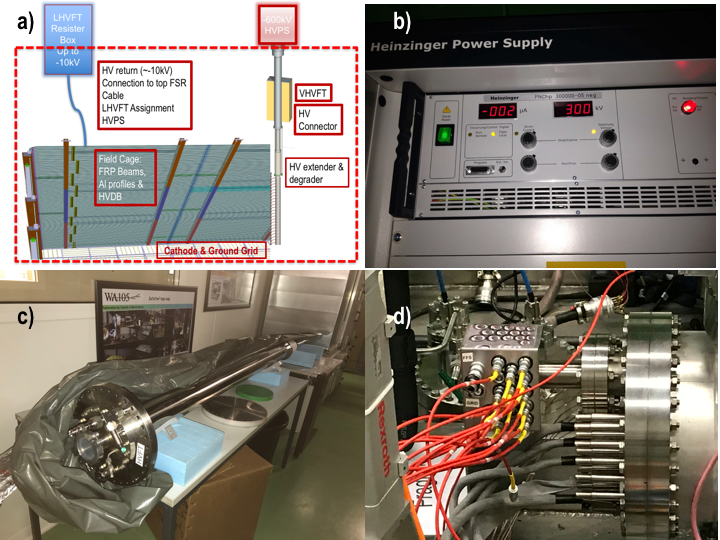
\includegraphics[width=1.0\textwidth,height=1.2\textwidth]{graphics/dp-hvs-n-photos.png}
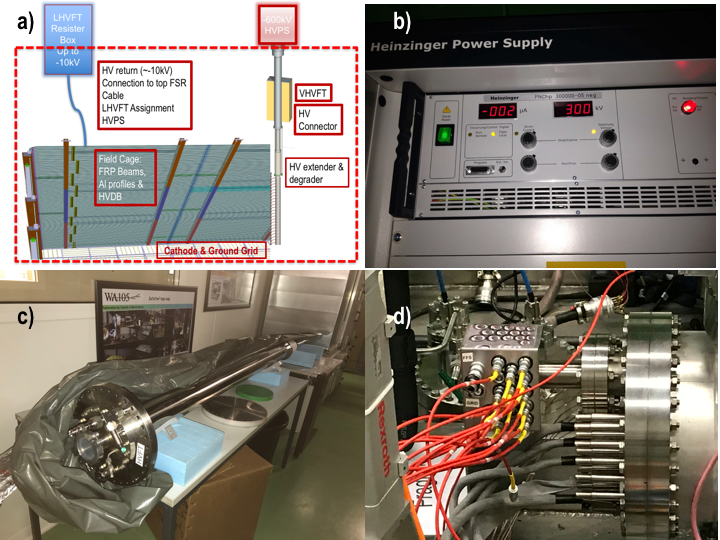
\includegraphics[width=0.8\textwidth]{DP_HVS_dp-hvs-n-photos.png}
\end{dunefigure}

The system operates at the full range of voltages, 
$-$\dptargetdriftvoltneg to ground \fixme{In the PDF, this appears to have two minus signs. Is that correct?}, inside the \dword{tpc} volume. 

The \single and \dual modules will use similar designs for some \dword{hv} system components, 
in particular, some aspects of the \dwords{fc} and their supporting beams. The \dword{dp} versions are described in this chapter. 
 %\fixme{for Anne  let's list sections where these components are described. Anne}.

The design presented in this chapter uses primarily the \dword{pddp}, \dword{pdsp}, and \dword{wa105} experiences. Scaling up from the size of these  prototypes presents some challenges that the \dune \dword{dpmod} is designed to meet: 

%\subsection{Design Considerations}

%Among the design considerations are many challenges scaling up the \dword{pddp} \dword{tpc} design to the \dword{dune} \dword{fd}. The most prominent ones are 
\begin{itemize}
    \item generating and transmitting the \SI{600}{\kV} voltage safely to the cathode plane \SI{12}{\m} below the liquid level;
    \item safely dissipating all the energy stored ($\sim$ \SI{3}{\kJ}) in the %entire 
    \dword{tpc} in the event of an \dword{hv} discharge; and 
    \item managing the dissimilar thermal contraction rates of the various component %different 
    materials over the \SI{60}{\m} length of the \dword{tpc}.
\end{itemize}

%\fixme{Fit this sentence in later: Generating and transmitting \SI{600}{\kV} to the cathode remain an R\&D item in collaboration with Heinzinger.}


%%%%%%%%%%%%%%%%%%%%%%%%%%%%%%%%%%%%%
\section{Design Requirements}
\label{sec:fddp-hv-des-consid}

The working principle of the \dword{lartpc} relies on applying a strong and  very uniform  \efield. A number of detector performance parameters benefit from such an \efield in ways that directly support the core components of the \dword{dune} physics program. 
%\fixme{not sure what prev sentence is saying. I think you could skip from 'ultra-pure Lar.' straight to next pgraph. anne} 
Some of these are examined in detail in \dword{tdr} Volume~\volnumberphysics{}, \voltitlephysics{}. 
Here we set the context by presenting a qualitative description of the \efield effects on physics.

Because free electron drift velocity in \dword{lar} is a function of the \efield, a uniform \efield allows mapping along the drift direction using simple time versus position and enables precise and efficient \threed reconstruction.  This allows, for example, establishing a well defined fiducial volume for %beam neutrino events reconstructed in the \dune \dword{dpmod}.  
reconstructing beam neutrino events in the \dune \dword{dpmod}. A neutrino \dword{cpv} %violation 
measurement, or a neutrino mass hierarchy test, %at root 
%basically 
compares normalized spectra for electron and muon neutrino and antineutrino interactions in the fiducial volume of the %\dword{fd}
\dune \dword{dpmod}, as projected from the \dword{nd}. For this reason, fiducial volume characterization is critical.   

Spectral information is necessary to separate \dword{cp} and \dword{mh} effects, necessitating efficient track and shower reconstruction and good energy resolution. Toward these ends, higher \efield strengths are generally better.  More free charge is created at the ionization points because recombination decreases at higher fields, improving \dword{s/n} and calorimetry. Drift times are reduced, resulting in less electron capture and better \dword{s/n}, even under less than optimal \dword{lar} purity conditions.  Spatial resolution improves as $\sqrt{t_{drift}}$-dependent diffusion effects decrease. %lessen. 
Higher free charge production and lower electron capture give lower detection thresholds on components of electromagnetic showers, improving shower energy reconstruction.  Lower detection thresholds also lead to higher detection efficiency for MeV-scale electron, photon, and neutron signatures of low-energy $\nu_e$ interactions from \dword{snb} events.  The decreased recombination affects highly ionizing particles, usually protons, more than \dwords{mip}. Less saturation of free charge production occurs, leading to better particle identification and more precise energy measurements. Lower recombination particularly helps proton-kaon separation by $dE/dx$, a key component of a search for $p\rightarrow K^+ \nu$ baryon decay events. 

However, apart from obvious technical limitations, the \efield should not be raised beyond certain limits. For instance, while free charge production increases with \efield, scintillation photon production decreases, resulting in fewer photons available for both triggering and establishing $t_{0}$. % purposes.
Two-track separation can degrade if drift velocity increases while the electronic waveform sampling frequency remains fixed. The distance between the \dword{tpc} boundaries and the cryostat walls would likely need to be increased for very high \efield{}s to prevent electrostatic discharge. This would, in turn, reduce the fraction of the \dword{lar} within the fiducial volume. The effects of the reduced number of photons
%\fixme{the first what? is it "fewer photons" first and "two-track separation degradation" second?}  
are modest, and all effects are subsumed by technical challenges in delivering \dword{hv} to the cryostat and maintaining highly stable \dword{hv} surfaces for long-term operation. 
%\fixme{several decades?} 
These challenges require developing non-commercial cryogenic \dword{hv} \fdth{}s, \dword{hv} ripple-repression through custom \dword{hv} \dword{r-c} circuits, careful construction and deployment of \dword{hv} cables, redundant \dword{hv} connections, high-precision monitoring, and best practices at all stages of design, installation, and operation.

Two decades of design and operational experience that began with ICARUS~\cite{icarus} have established that a \SI{500}{\V/\cm} field is an appropriate trade-off value that can be realistically achieved using cost-effective design and construction methods. Achieving this design goal in the \dune \dword{dpmod} %will be challenging because the drift distance has progressively increased to the \SI{12}{m} foreseen for the \dune \dword{dpmod} (6m drift), and overall detector optimization has proven important. (Anne)
will be challenging because of the \SI{12}{m} drift distance and the importance of overall detector optimization. 
The forthcoming test of \dword{pddp} will likely run at the nominal \dword{hv} of \SI{-300}{\kV} applied on the cathode. Its successful operation will confirm that the \dune \dword{dpmod} can operate at least at E=\SI{250}{\V/\cm}. 
However, %DUNE must be able to run at higher voltage,
it must be able to run at an \efield of up to the nominal \SI{500}{\V/\cm} %field 
(\dword{hv} of \SI{-600}{\kV}) to compensate for unexpectedly low-purity conditions that could arise over two decades of planned operation. 
%\fixme{is the -300 vs +500 significant? I think including the neg sign with 300 just serves to confuse}

%\fixme{(It would be better if we could cite ProtoDUNE)} 
The \SI{500}{\V/\cm} \efield goal, combined with high \dword{lar} purity, a large \dword{s/n} ratio, and a large \dword{crp} gain, will allow a wide range of possible operating points to optimize detector performance 
%\fixme{in other words you can choose from a number of different combinations of these parameters to find one or some that optimize(s) performance? (I added "two" before 'decades'.) Anne}
for maximum physics potential over two decades of stable conditions and very high live time. 
%\fixme{some duplications in the paragraph above and below - BY}
This value is therefore set as the goal. 
%The specifications for the \dword{dune} \dword{dp} \dword{hv} system thus have the goal of \SI{500}{\V/\cm}, pointed  toward the highest possible detector performance and widest span of operating points, and a minimum 
The value for minimal acceptable detector performance is \SI{250}{\V/\cm}, assuming the purity and electronics specifications are achievable. %parameters. 

Unlike the \dword{sp}, in the \dword{dp} detector space charge could %be non-negligible in distorting the \efield %uniformity 
distort the \efield to a non-negligible degree 
because of the presence of the irreducible \Ar39 radioactive background that constantly produces positive ions in \dword{lar} and the long drift distance that prolongs their %permanence 
presence in the drift volume. %In addition, this effect could be highly enhanced by the injections into \dword{lar} of the positive ions produced by the electron multiplication in the \dword{lem} amplification stage (up to a factor \num{20} at nominal \dword{lem} gain). 
Injections into \dword{lar} of positive ions produced by the electron multiplication in the \dword{lem} amplification stage (up to a factor \num{20} at nominal \dword{lem} gain) could significantly enhance this effect. 
%To mitigate this effect, the \efield in the drift region must be as high as possible, which allows speeding up positive ions in \dword{lar} toward the cathode where they are neutralized, thus reducing the overall space charge. Hence, the goal of reaching the nominal value of \SI{500}{\V/\cm} is much more important for the \dword{dp} case, in spite of the higher technological challenge of applying \SI{-600}{\kV} on the cathode. 
To reduce the overall space charge, the \efield in the drift region must be kept as high as possible to drift the positive ions more quickly toward the cathode where they are neutralized. This underlines the importance of reaching the nominal value of \SI{500}{\V/\cm} in the \dword{dpmod} despite the greater challenges. 
%Hence, the goal of reaching the nominal value of \SI{500}{\V/\cm} is much more important for the \dword{dp} case, in spite of the higher technological challenge of applying \SI{-600}{\kV} on the cathode.

The \dword{hv} system is designed to meet the physics requirements of the \dword{dune} experiment. This includes both physical requirements (e.g., an \efield 
that allows robust event reconstruction) and operational requirements (e.g., 
avoiding over-complication that could compromise %to maximize 
data collection efficiency). 
Table~\ref{tab:specs:DP-HV} provides a collection of essential specifications for
the \dword{hv} system.
We have chosen the convention of referring to electric field strength in the requirement table.
%{tab:hvphysicsreqs}.
%\fixme{need generated spec table}

% This file is generated, any edits may be lost.
\begin{footnotesize}
%\begin{longtable}{p{0.14\textwidth}p{0.13\textwidth}p{0.18\textwidth}p{0.22\textwidth}p{0.20\textwidth}}
\begin{longtable}{p{0.12\textwidth}p{0.18\textwidth}p{0.17\textwidth}p{0.25\textwidth}p{0.16\textwidth}}
\caption{Specifications for DP-HV \fixmehl{ref \texttt{tab:spec:DP-HV}}} \\
  \rowcolor{dunesky}
       Label & Description  & Specification \newline (Goal) & Rationale & Validation \\  \colhline

   \newtag{DP-FD-1}{ spec:dp-min-drift-field }  & Minimum drift field  &  $>$\,\SI{250}{V/cm} \newline ( $>\,\SI{500}{V/cm}$ ) &  Lessens impacts of $e^-$-Ar recombination, $e^-$ lifetime, $e^-$ diffusion and space charge. &  ProtoDUNE \\ \colhline
    
   
  \newtag{DP-FD-11}{ spec:dp-hvs-field-uniformity }  & Drift field uniformity due to HVS  &  $<\,\SI{1}{\%}$ throughout volume &  High reconstruction efficiency. &  ProtoDUNE and simulation \\ \colhline
    
   
  \newtag{DP-FD-12}{ spec:dp-hv-ps-ripple }  & Cathode HV power supply ripple contribution to system noise  &  $<\,\SI{100}e^-$ &  Maximize live time; maintain high S/N. &  Engineering calculation, in situ measurement,   ProtoDUNE \\ \colhline
    
   \newtag{DP-FD-17}{ spec:dp-cathode-resistivity }  & Cathode resistivity  &  $>\,\SI{1}{\mega\ohm/square}$ \newline ($>\,\SI{1}{\giga\ohm/square}$) &  Detector damage prevention. &  ProtoDUNE \\ \colhline
    
   
  \newtag{DP-FD-24}{ spec:dp-local-e-fields }  & Local electric fields  &  $<\,\SI{30}{kV/cm}$ &  Maximize live time; maintain high S/N. &  ProtoDUNE \\ \colhline
    

   \newtag{DP-HV-1}{ spec:hvdb-redundancy }  & Provide redundancy in HV distribution  &  $>\,num{2}$ HVDB chain \newline (\num{12} HVDB chains) &  Ensure the HV connections to the detector &  ProtoDUNE and calculations \\ \colhline
    


\label{tab:specs:DP-HV}
\end{longtable}
\end{footnotesize}

\begin{comment}
\begin{dunetable}
[\dshort{hv} system requirements]{p{0.05\textwidth}p{0.2\textwidth}p{0.35\textwidth}p{0.15\textwidth}p{0.15\textwidth}}
{tab:hvphysicsreqs}
{\dword{hv} System Requirements.}
No. & Requirement & Physics requirement driver & Requirement & Goal \\ \toprowrule
1 & Exceed minimum \efield TPC drift volume & Maintain adequate particle ID, which is affected by slower drift speed and increased recombination, diffusion, and space charge. & >\SI{250}{V/cm} &\SI{500}{V/cm} \\ \colhline
 2 & Do not exceed maximum \efield in \lar volume & Avoid damage to detector to enable data collection over long periods. & \SI{30}{kV/cm} & \dword{alara} \\  \colhline
3 & Minimize power supply ripple & Keep readout electronics free from external noise. %, which confuses event reconstruction.  
\\ \colhline
4 &  Maximize power supply stability & Maintain the ability to reconstruct data taken over long periods.  Maintain high operational up time to maximize experimental statistics. \\ \colhline
5 & Provide adequate decay time constant for discharge of the cathode plane and \dword{fc} as well as cathode plane resistive segmentation & Avoid damage to detector to enable data collection over long periods. Maintain high operational up time to maximize experimental statistics. & \si{\giga\ohm} resistors per each connection of the $4\times12$m$^2$ cathode units and \dword{fc} super-modules \\ \colhline
6 & Provide redundancy in all \dword{hv} connections & Avoid single-point failures in detector that interrupt data taking. & > 2 voltage divider chains to distribute \dword{hv} to the \dword{fc} profiles & one voltage divider chain every four \dword{fc} modules which form a super-module\\ 
\end{dunetable}
\end{comment}


%\clearpage
%%%%%%%%%%%%%%%%%%%%%%%%%%%%%%%%%%%%%%%%%%%%%%%%%%%%%%%%%%%%%%%%%%%%
\section{ProtoDUNE-DP Experience}
\label{sec:fddp-hv-protodune}
%\subsection{Summary of Construction and Operation - 1 page }
%\label{sec:fddp-hv-protodune-summary}
%%%%%%%%%%%%%%%%%%%%%%%%%%%%
%\fixme{AH: I'd like to see the \dune \dword{dpmod} described first, then the protodune part after. Maybe we can discuss. - yes JY}


%The \dword{pddp} detector was designed to cover \SI{6}{\m} $\times$ \SI{6}{\m} $\times$ \SI{6}{\m} active volume. This enabled testing the concept of scalable final detector components, in particular the \dword{crp}. the cathode, and the \dword{gg} whose unit component dimensions are \SI{3}{\m} (W) $\times$ \SI{3}{\m} (L). The \dword{fc} of the \dword{pddp} surrounds the \SI{6}{\m} $\times$ \SI{6}{\m} $\times$ \SI{6}{\m} active volume, so the testing was effectively done using the concept that the combination of the \SI{3}{\m} (W) $\times$ \SI{2}{\m} (H) sub-modules make up an \dword{fc} module of dimension \SI{3}{\m} (W) $\times$ \SI{6}{\m} (H). The HV applied to the cathode was at maximum \SI{-300}{\kV} to provide a \SI{500}{\V/\cm} drift field to the \SI{6}{\m} drift length. The sub-module assembly procedure and the subsequent installation procedure were tested in the cryostat and can be applied to \dword{dune} with some minor changes to reflect the lessons learned from \dword{pddp} installation.  
The \dword{pddp} detector has a \SI{6}{\m} $\times$ \SI{6}{\m} $\times$ \SI{6}{\m} active volume. This allowed testing the final detector components at scale, in particular the \dword{crp}, cathode, and \dword{gg}, whose unit dimensions are \SI{3}{\m} (W) $\times$ \SI{3}{\m} (L). The \dword{fc}, which surrounds the active volume, comprises modules of dimensions \SI{3}{\m} (W) $\times$ \SI{6}{\m} (H); these in turn comprise \SI{3}{\m} (W) $\times$ \SI{2}{\m} (H) submodules.  The \dword{hv}{} applied to the cathode is at maximum \SI{-300}{\kV} to provide a \SI{500}{\V/\cm} drift field to the \SI{6}{\m} drift length.  
The \dword{fc} submodule assembly procedure and the subsequent installation procedure tested in the cryostat can be applied to the \dune \dword{dpmod} with some minor changes to reflect the lessons learned from \dword{pddp}. 

\fixme{anne would remove this - there's lots of other info you're giving} The \dword{pddp} detector is not in operation at the time of this writing, so we can only provide information on the air commissioning (see Section~\ref{sec:fddp-hv-protodune-air}).


\subsection{Design}
\label{sec:fddp-hv-protodune-lessons-design}
%The design of the \dword{pddp} \dword{fc} sub-modules used two \SI{15.2}{\cm} (\SI{6}\,in) FRP I-beams connected by two \SI{7.6}{\cm} (\SI{3}\,in) FRP I-beam cross bars, to form a frame. The two \SI{15.2}{\cm} (\SI{6}\,in) FRP I-beams have slots conforming to the shape of the aluminum profiles in which they are inserted. Since the mechanical connections between the sub-modules use \SI{10}{\cm} wide G10 plates exterior to the active volume as well as the (\SI{3}\,in) FRP I-beam cross bars, a large fraction of insulators from the FRP frame structure is exposed toward the cryostat membrane wall at ground. The design of the \dword{fc} sub-module has been changed to minimize insulator exposure toward the cryostat membrane wall to reduce the potential source for unexpected streamers which were observed in \dword{pdsp} operations.  With this change, the new design for \dword{dune} has no insulators exposed toward the wall, leaving all inter-sub-module mechanical connections inside the active volume, away from the walls. Furthermore, to reduce the drift field distortion from surface charge accumulation, the cross bars are replaced with stainless steel tubes as described in detail in Section~\ref{sec:dp-hv-system-fc}.

The \dword{pddp} \dword{fc} submodules consist of two \SI{15.2}{\cm} (\SI{6}\,in) \dword{frp} I-beams connected by two \SI{7.6}{\cm} (\SI{3}\,in) \dword{frp} I-beam cross bars to form a frame. The two \SI{15.2}{\cm} (\SI{6}\,in) I-beams have slots conforming to the shape of the aluminum profiles into which they are inserted. Because the mechanical connections between the submodules use \SI{10}{\cm}-wide G10 plates exterior to the active volume as well as the (\SI{7.6}{\cm}) I-beam cross bars, a large fraction of the insulators from the \dword{frp} frame structure is between the \dword{fc} electrode and the cryostat membrane wall at ground. 

The \dword{dune}{} \dword{dpmod} \dword{fc} submodule design has been changed so all inter-submodule mechanical connections are inside the active volume, away from the cryostat walls, to reduce the potential for streamers, which were observed in \dword{pdsp}. Furthermore, to reduce the drift field distortion from surface charge accumulation, the cross bars are replaced with stainless steel tubes (see  Section~\ref{sec:dp-hv-system-fc}).

Two \dword{pddp} design features raised significant concerns about the risk of discharging a large amount of stored energy toward the membrane wall or the floor:  (1) the aluminum profile electrodes that form an electrically continuous field-shaping ring and  interconnected with aluminum clips, and (2) the use of all stainless steel tubes in the cathode construction. A large  discharge could seriously damage the cryostat wall, disable detector operations, and cause a significant safety hazard. 
To address these safety concerns, in the \dword{dune} \dword{dp},  the metal profile clips are replaced with resistive sheaths as described in Section~\ref{sec:dp-hv-system-fc}, and the cathode modules are made of resistive tubes held by metal trusses as described in  Section~\ref{sec:dp-hv-system-cathode}.

The \dword{pddp} resistive \dword{hv}{} divider boards shown in Figure~\ref{fig:pddp-hvdb} a-c are designed to provide the desired voltage difference between two adjacent field-shaping rings. 
Most of these boards cover nine gaps. 
The two boards that connect the cathode to the \dword{fc} cover eight  gaps because of %the chose \fixme{choice?} of the 
the total number of field-shaping rings. % in \dword{pddp}.
%\fixme{This is not entirely clear because the two types of resistive VHV divider boards are not named. In addition, pairing up the divider boards with the respective gaps would be clearer than using the phrasing necessary to "respectively."  Resistive VHV divider board X is designed to cover \num{9} gaps, and resistive VHV divider board Y is designed to cover \num{8} gaps. See Figure~\ref{fig:pddp-hvdb}.}
The design of the \dword{hv} divider board %called for 
implements ample redundancy.  
Each gap between the adjacent field-shaping rings has two \SI{2}{\giga\ohm} main resistors for the voltage drop and four varistors to accommodate up to \SI{6}{\kV}, twice the operation voltage, in case the final \SI{600}{\kV} \dword{hvps} becomes available.
\dword{pddp} uses two rows of \dword{hvdb} for additional redundancy, taking advantage of the electrically continuous field-shaping rings.
The board design will change slightly for the \dune \dword{dpmod} to minimize the potential for a discharge between the solder balls on the back of the board, as shown in Figure~\ref{fig:pddp-hvdb}c, that are exposed between the two adjacent field-shaping rings. 
In addition, because the operational voltage difference will not exceed \SI{3}{\kV} between the two adjacent profiles, the number of varistors will be reduced from four to two, significantly simplifying the design of the board and potentially eliminating the exposed solder balls.

\begin{dunefigure}[\dual HV divider board]{fig:pddp-hvdb}{\dword{pddp} \dword{hv} divider board: (a) schematic circuit diagram, (b) photograph of the top of the board, and (c) photograph of the bottom of the board.}
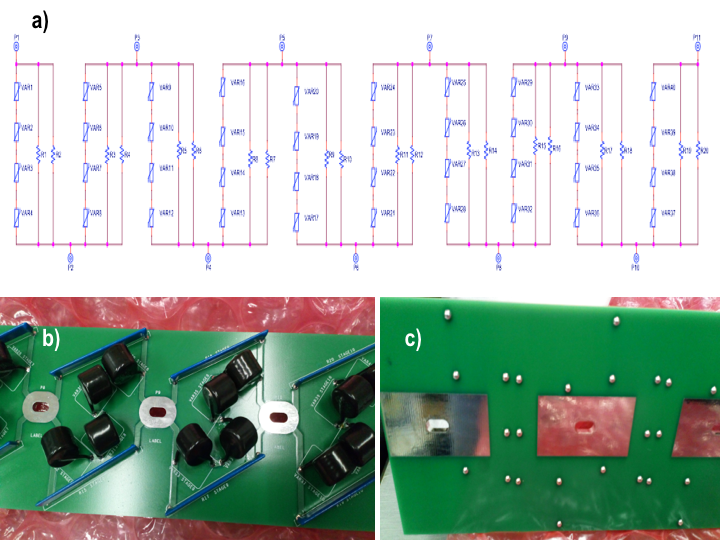
\includegraphics[width=0.75\textwidth]{DP_HVS_dp-hvdb.png}
\end{dunefigure}

%\begin{dunefigure}[\dual \dword{hvdb}]{fig:pddp-hvdb}{\dword{pddp} %\dword{hv} divider board (a) schematic circuit diagram, (b)photo of the top of the board, (c) photo of the bottom of the board}
%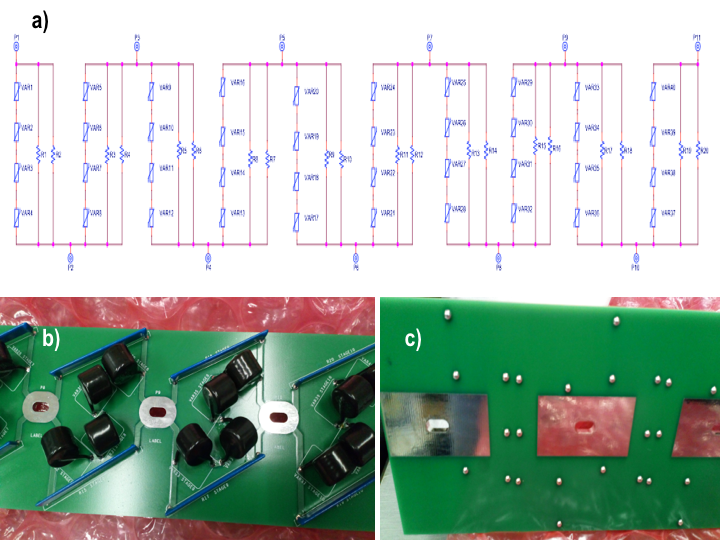
\includegraphics[width=0.75\textwidth]{graphics/dp-hvdb.png}
%\end{dunefigure}
%\fixme{(anne) this figure is referenced in several places but whole figure was commented out. Figure out what to do about figure.}

\subsection{Construction}
\label{sec:fddp-hv-protodune-lessons-construction}
The \dune \dword{dpmod} will follow the construction process of the \dword{pddp}, which worked out well. 
For \dword{qa} and \dword{qc}, the vendor-machined \dword{frp} parts for the \dword{fc} are processed at the factory to eliminate burrs and defects left on the parts.   
These parts are then cleaned using de-ionized water and colorless Simple Green \footnote{https://www.simplegreen.com}, and dried in a humidity-controlled storage room.
Once the \dword{frp} I-beam parts are dried, the processed surfaces % areas 
are covered with polyurethane varnish for further suppression of any remaining fiber on their edges. % of them. 
The parts are then brought to a humidity-controlled cleanroom (class $\sim\,$10,000), assembled as a frame to ensure mechanical fitness, then  disassembled and packaged compactly to the dimensions \SI{0.2}{\m} (W) $\times$ \SI{0.2}{\m} (H) $\times$ \SI{2}{\m} (L), and wrapped in plastic shrink wrap for storage before shipment.
%This process worked out well in \dword{pddp}, so the same process will be followed in \dword{dune} \dual as well.
The design change made for \dune \dword{dpmod} makes it significantly easier to process and condition the \dword{frp} parts because the \dword{frp} I-beams no longer have slots conforming to the profiles, eliminating the time-consuming machining and cleaning process.
In addition, the package for each submodule will be far more compact than the \dword{pddp} \dword{fc} submodules because the width of the I-beams is \SI{10.2}{\cm} (\SI{4}\,in). As a reference, Figure \ref{fig:dune-dp-fc-all} shows the main \dword{fc} components and connections for \dword{pddp}.

\begin{dunefigure}[Field cage parts]{fig:dune-dp-fc-all}
{\dword{fc} parts and connections for \dword{pddp}:  a. One \SI{3}{\m} (W) $\times$ \SI{6}{\m} (H) \dword{pddp} \dword{fc} module with three \SI{3}{\m} (W) $\times$ \SI{2}{\m} (H) submodules.  The \dune \dword{dpmod} has a nearly identical structure except for the number of middle submodules (four) and the profile length (\SI{4}{\m} instead of \SI{3}{\m} in \dword{pddp}); b. A photograph of the top module connection to the stainless steel I-beam and an inter-submodule connection; c. Aluminum clip connections in the corner and in the straight sections.  These clips will be replaced with resistive sheaths in \dune \dword{dpmod} to increase the decay time in case of discharge; d. \dword{hv} divider boards and their connections on \dword{pddp} \dword{fc}.}
%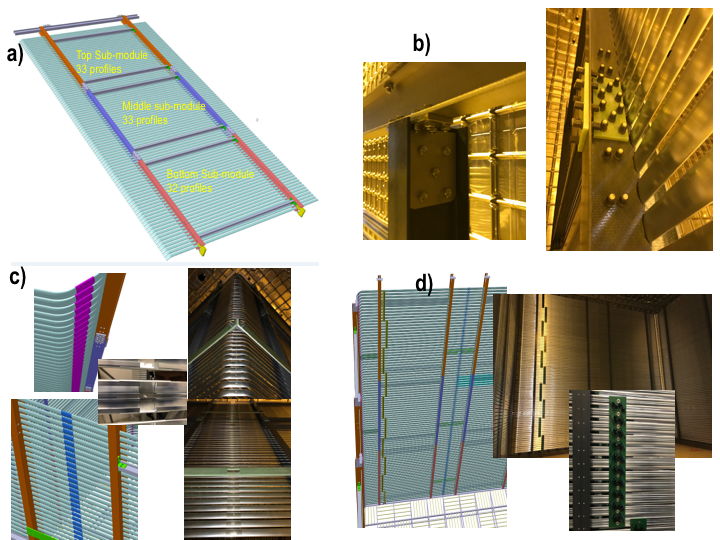
\includegraphics[width=1.0\textwidth,height=1.0\textwidth]{graphics/dp-fc-parts.png}
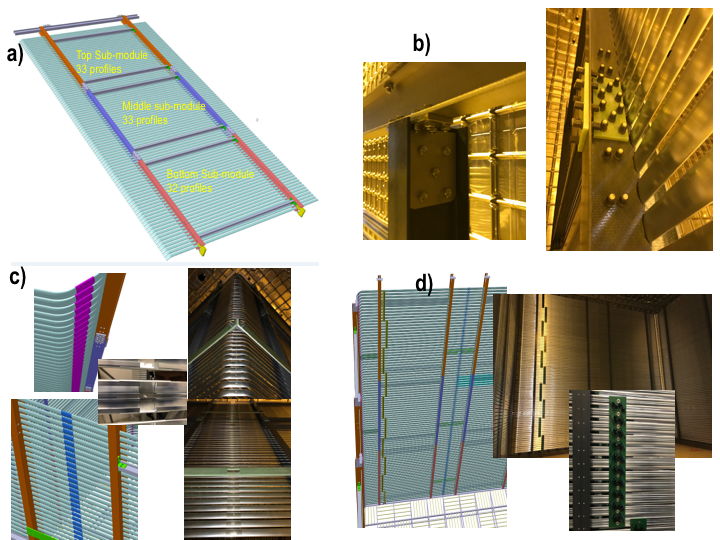
\includegraphics[width=0.9\textwidth]{DP_HVS_dp-fc-parts.png}
\end{dunefigure}

The resistor and varistor parts for the \dword{pddp} \dwords{hvdb} were tested in air while warm, in \lntwo and then again in air after warm up to ensure the quality and resilience of the parts.  
Based on these measurements, parts were selected to ensure resistance values within \num{1}\% of the mean. 
The selected parts were shipped to the contractor to be mounted on the \dword{pcb} with through holes that allow soldering on the back of the board.
The boards with resistors mounted on them were then tested again for \dword{qc}, twice in air and once in \lntwo; if any of the gaps failed the \dword{qc} criteria, the board was rejected and sent back to the manufacturer to replace the parts in the failed gap.
The same \dword{qc} process will be used for the \dword{dune}{} \dword{dpmod}.

The \dword{pddp} \SI{3}{\m}$\times$ \SI{3}{\m} cathode units were built out of stainless steel tubes welded together in a structure that ensures more than \num{90}\% light transparency.
To slow down energy release from an unexpected discharge in \dword{pddp}, resistor boards were built to interconnect two neighboring cathode units. 
This resistor network, however, affected the input voltage to the \dword{hvdb} row diagonally across the \dword{fc} panel that accepts \dword{hvps} input, so the bottom-most gap of the \dword{hvdb} row was modified to compensate for the voltage drop across the diagonal connection from the \dword{hv} input. 
%This choice to implement resistors, and thus slow down energy release, has been taken into account in \dword{dune} \dual cathode design, as described in Section~\ref{sec:dp-hv-system-cathode}.
The \dword{dune} \dword{dpmod} cathode will also implement resistors, as described in Section~\ref{sec:dp-hv-system-cathode}.

\subsection{Assembly and Installation}
\label{sec:fddp-hv-protodune-lessons-assy}

The \dword{fc} submodules are built in the cleanroom %buffer 
in front of the \dword{tco} of the \dword{pddp} cryostat.
The assembly of each submodule, including inserting and securing the profiles onto the \dword{frp} frame, should take two people approximately two hours.
When as many submodules are built as the cleanroom %buffer 
storage space allows, they are brought into the cryostat for installation.
Installing each \SI{6}{\m} (H) $\times$ \SI{3}{\m} (W) full length module begins with hanging the top submodule to a $\sim$ \SI{3}{\m} stainless steel I-beam attached to the stainless steel cable through \fdth in the ceiling.
The next submodule is then hung from the top module, and the third hung from the second submodule. \fixme{Two things here. I believe this should be in present tense. Second, check the sequence. I think the second submodule is hung from the first, and the third from the second.}
The whole installation process for a \SI{6}{\m} module takes  four people approximately an hour, with two people inside the cryostat connecting the modules while the other two are on top of the cryostat roof, operating winches that raise the corresponding partial module as successive submodules are attached.

This scheme requires two \fdth holes per module, which makes the total number of \dword{fc} installation \fdth holes large. Figure~\ref{fig:dp-fc-installation-connection} shows the two submodules connected and hanging from the two sets of stainless steel cables on the ceiling (left) and the inter-submodule connections (right).

\begin{dunefigure}[\dual FC installation process and inter-module connection]{fig:dp-fc-installation-connection}{Left: Two submodules connected and hanging from the two sets of stainless steel cables on the ceiling.  The lifting wires raise the module to its position as submodules are connected; the hanging wires keep the fully integrated module in its final position.  Right: Inter-submodule connections.  Each connection is made with two \SI{1}{cm} thick G10 plates along the height of the I-beams and one \SI{1}{cm} thick G10 plate on the flange.}
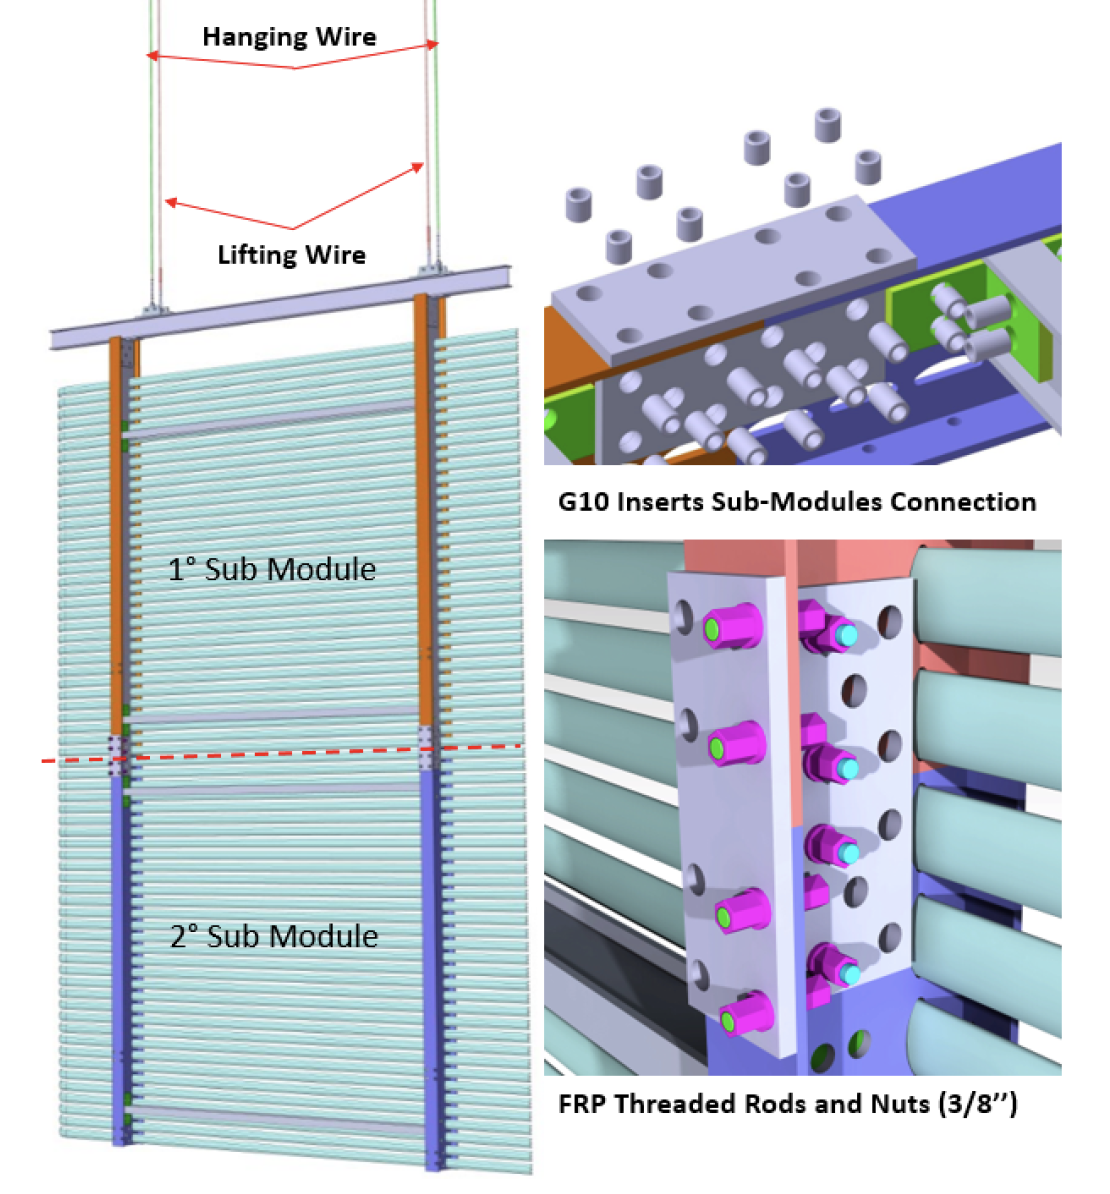
\includegraphics[width=0.75\textwidth]{DP_HVS_module-connection-installation.png}
\end{dunefigure}

A modified installation plan has been developed to reduce the number of \fdth holes by a factor of 4 and reduce the number of parts needed for the \dword{fc} modules, as described in Section~\ref{sec:dp-hv-system-fc}, thus simplifying installation and saving costs.

The \SI{3}{\m} (L) $\times$ \SI{3}{\m} (W) \dword{pddp} cathode and \dword{gg} modules are preassembled outside of the cleanroom %buffer 
and brought into the cryostat for installation.
The assembly and installation scheme for the \dword{dune} \dword{dp} cathode must also change because its structure and  material composition are modified to increase the time for energy release by several orders of magnitude. As demonstrated by the study performed for \dword{sp} cathode, %with the final goal of protecting 
this protects the cryostat membrane from potential damage. \fixme{Check this for correctness please.}

%\subsection{Performance}
%\label{sec:fddp-hv-protodune-lessons-perf}

%The \dword{pddp} detector is not yet in operation at the time of this writing, so we can provide no input on performance other than the air commissioning we have performed and summarized in the next section.
%%%%%%%%%%%%%%%%%%%%%%%%%%%%

%\subsection{Lessons from ProtoDUNE}
\subsection{Pre-\cooldown Commissioning Test}
\label{sec:fddp-hv-protodune-air}

%\fixme{this is what anne understands:}
%Once FC was completely installed but before installation of other detector components, you wanted to test the electrical response of the FC and see if you could hold 150kV.  
%You made all the connections (using the same equipment and technique as you will when you're ready to connect them for actual operation?). You held the voltage (success), but the current rose too high (not good). Your camera looked for sparks, but you don't say if you saw any. You suspected a surface layer of water on the FRP that the current flows through. So to test, you took a separate piece of FRP, hooked it up and got same result. But it worked fine in LAr.  You still want to investigate the water adhesion properties of FRP from different manufacturers because you don't want this surface current problem to occur even in air.
%\fixme{end Anne's blurb. Please correct or confirm my understanding. Once I understand better, I can edit the below better. ==> yes, exactly.  We did not see any sparks at all. JY}

To ensure the performance of the \dword{fc} and to identify any issues well before the final installation of the other detector pieces, the \dword{pddp} \dword{fc} is connected to a \SI{150}{\kV} power supply for an air commissioning test. The entire \dword{fc} was fully installed and connected; slip nuts were used for inter-module connections to provide electrical continuity. 
Because the electrical interconnections were made to each %of the 
field-shaping ring, 
%\fixme{connections betw rings or modules? anne}
the resistance between %\fixme{each set of two?} 
the two neighboring rings is measured and compared to the expected values to verify the connection.
The \SI{150}{\kV} \dword{hv} is fed into the two middle field-shaping rings along the height of the \dword{fc}. This ensures 
%\fixme{this 'set' the voltage diff?} 
a voltage difference between any two neighboring rings of \SI{3}{\kV} (the operational voltage) when the top-most and bottom-most rings are connected to the ground on the membrane wall.

An online wide-angle camera is placed on the floor at the corner where the \dword{hv} feeds in to ensure any possible sparks can be seen.
No sparks have been observed by the camera.
Current and voltage are carefully monitored and recorded to make sure any discharge can be observed and studied.
When the \dword{hv} was turned on for the first time, %we observed the current settled after the charge up was about \num{50}\% higher than expected.
the current settled at about \num{50}\% higher than expected after the full charge up.
Voltage remained on for many hours to monitor the long-term behavior of the \dword{fc}.
The current continually increased to higher, unexpected  values several times %while the testing was carried 
through multiple power cycles.
A systematic test revealed that the size of the current read back was directly proportional to the number of \dword{fc} modules independent of the magnitude of the current.

This %test pointed in the direction of the \dword{frp} beams, leading 
result leads to the hypothesis 
\begin{comment}
that the ambient humidity %allowed 
allowed a layer of water %to cover 
to form on the surface of the \dword{frp} beams  through which % and 
the current flowed. % through this water layer.
\end{comment}
Thus, the current flows through a layer of water on the surface of the \dword{frp} beams due to the ambient humidity.

%Resistance measurements of a \SI{50}{\cm} long \SI{15.2}{\cm} (\SI{6}{in}) wide I-beam sample piece in air with similar  humidity and in \dword{lar} showed that while the current in air was consistent with what was observed for \dword{pddp} \dword{fc}, the resistance showed expected values with virtually no surface current flowing through once the \dword{frp} I-beam is in \dword{lar}. Since this behavior was not observed in \dword{pdsp} \dword{fc} which was under the similar humidity environment, we suspect that the \dword{frp} beams from a different manufacturer may have different surface water adhesion properties. Thus, it may be necessary to study the \dword{frp} beam from the current manufacturer in further detail for \dual \dword{fc}.
Resistance measurements of a \SI{50}{\cm} long, \SI{15.2}{\cm} (\SI{6}{in}) wide I-beam sample piece were made in air at roughly the same humidity level and in \dword{lar}. The measurements in air were consistent with the \dword{pddp} \dword{fc} results,  but in \dword{lar}, the resistance showed expected values with almost no surface current. 
Because this behavior was not observed in the \dword{pdsp} \dword{fc}, which operated under a similarly humid environment, we suspect that the \dword{frp} beams from  different manufacturers may have different surface water adhesion properties. Thus, it may be necessary to study the \dword{frp} beam from the current manufacturer in further detail for the   \dword{dpmod} \dword{fc}.

Please note that the \SI{600}{\kV} power supply does not exist at the time of writing this report, so we are unable to test the system with the final power supply.
For this reason, we have added developing and testing a \SI{600}{\kV} power supply as a future R\&D item, as listed below.

\subsection{Suggestions for future R\&D}
\label{sec:fddp-hv-protodune-rd}
Experiences from constructing, assembling, installing, and air commissioning the \dword{hvs} at \dword{pddp} suggest the following R\&D items:

\begin{itemize}
    \item testing \dword{frp} surface-water adhesion property,
    \item using resistive sheaths instead of aluminum clips, 
    %\fixme{what about it?}
    \item determining distance between two neighboring profiles,
    \item investigating optimal resistance for delaying energy releases, and 
    \item generating and transmitting \SI{600}{\kV} to the cathode safely in collaboration with Heinzinger.
\end{itemize}


%%%%%%%%%%%%%%%%%%%%%%%%%%%%%%%%%%%%%%%%%%%%%%%%%%%%%%%%%%%%%%%%%%%%

\section{HV System Design}
\label{sec:fddp-hv-design}

The structural elements of the \dune \dword{dpmod} cathode and \dword{fc} resemble a rectangular wire basket (see Figure~\ref{fig:dune_dp_fd_hvs}). The \dword{hv} system components are summarized in Table~\ref{tab:specs:DP-HV}. The vertical \dword{fc} members are made of \dword{frp} beams, and the horizontal members are made of stainless steel. The cathode (the bottom of the basket) comprises 15 pairs of 12\,m long stainless steel trusses interconnected by stainless steel tubes at the bottom edges of the \dword{fc}. Stainless steel I-beams support the \dword{fc} from above; they are tied together to form a rigid rectangular frame.  

%\fixme{Anne still working through this - I think we can make this intro section shorter 4/3/19}


\begin{longtable}[HV system components]
{p{0.2\textwidth}
p{0.2\textwidth}
p{0.07\textwidth}
p{0.07\textwidth}
p{0.07\textwidth}
p{0.1\textwidth}
p{0.08\textwidth}}
\caption[HV system components]{\dword{hv} system components. Dimensions are given relative to the \SI{60}{m} length (L), \SI{12}{m} width (W), and \SI{12}{m} height (H) of the cryostat.}\\

Item & Arrangement & L & W & H & Components & Grand Total \\ \toprowrule
\dword{hvps} & atop cryostat on \fdth &   &  &  &  & 1 \\   \colhline
\dword{hv} \fdth{}s & &   &  &  &  & 1 \\   \colhline
\dword{hv} extender and voltage degrader &  runs vertically down from \fdth &   &  & 12\,m &  & 1 \\   \colhline
\dword{hvdb} row - each row draws \SI{3}{\micro\ampere}&  runs vertically down each super-module &   &  &  &  & 12 \\   \colhline
\dwords{hvdb} & 18 11-gap \dwords{hvdb} and one 1-gap \dwords{hvdb} per super-module &   &  &  &  & 216 + 12  \\   \colhline
Degrader rings &  installed on voltage degrader, 1 per field-shaping ring &   &  &  &  & 199 \\   \colhline\dword{hv} return \fdth{}s & &   &  &  &  & 1 \\   \colhline
Resistor box & &   &  &  &  &  1\\   \colhline

Cathode modules & 1 W $\times$ 15 L (horiz) &\SI{4}{m} &\SI{12}{m} & - & - & 15 \\   \colhline
Cathode trusses & two per cathode module, run along cryostat width (horiz)&   & \SI{12}{m} &  &  & 30 \\   \colhline
\Dword{gg} modules & 4 W $\times$ 20 L (horiz)&  \SI{3}{m}  & \SI{3}{m} & &  & 80 \\   \colhline
Resistive \dword{frp} rods in cathode & 122 per cathode module, run along length (horiz), threaded through trusses &   &  &  &  &  1,830\\   \colhline
HV cable segments in bus & inside the cathode outer tubes &   &  &  &  &  TBD \\   \colhline

field-shaping rings &   & 2$\times$\SI{60}{m}  & 2$\times$\SI{12}{m} &  &  & 199 \\   \colhline
Profiles  & 33 (stacked) per \dword{fc} submodule (34 on bottom submodules) & \SI{4}{\m} &  &  &  & 6,368 (straight) + 796 ($90^o$ bent)\\   \colhline

\dword{frp} beams in \dword{fc}  & two per \dword{fc} submodule & \SI{2}{\m}& \SI{5}{\cm} & \SI{10}{\cm} &  & 432 \\   \colhline

\dword{fc} submodules  &90 per long side, 18 per end (vert)&   & \SI{4}{m} & \SI{1.98}{m} & - & 216 \\ \colhline

\dword{fc} modules  & 15 L, three W (vert) &    &  4 m & 12 m & six stacked submodules & 36 \\ \colhline
\dword{fc} super-modules & five per long side, 1 per end (vert) &  & \SI{12}{m} & \SI{12}{m} & three adjacent \dword{fc} modules & 12 \\
\label{tab:hvcomponents}
\end{longtable}
%\clearpage
%\fixme{Please fill in table! I took it from SP HV and started to fill in. Anne}


%Anne replaced this text: For the \dual \dword{fd} \dword{hvs}, we are adopting a concept partially similar to that developed in the \single \dword{tpc} \dword{hv} system design, in which the \dword{fc} is built in independent modules, as much as possible equal to each other. Contrary to the \single case, however, the aluminum profiles mounted in the modules will be electrically connected together through resistive elements to form full 144 m long equi-potential rings surrounding the drift volume.
%\fixme{JY to Bo and Francesco: What concept from \single does the \dual adopting?  Certianly not the electrical isolation between the modules.}
%As in the \dword{sp}  case, the cathode will be made entirely of highly resistive material. However, to make it transparent to the scintillation light detectors placed below the cathode, it will be made of \dword{frp} bars laminated with resistive kapton (similar materials as the ones used for the \single CPA). The implementations for the \dword{fc} and cathode are summarized as follows.
% ---Move to FC subsection. AH --- Similar to the \dword{spmod}, the \dune \dword{dpmod} \dword{fc} is modular, with sections as similar to each other as possible, and the cathode will be made entirely of \dword{frp} laminated with highly resistive kapton. Adjacent aluminum profiles of the \dword{fc} modules will be electrically connected by resistive elements to form the full \SI{144}{m}-long equipotential rings that run the full perimeter of the drift volume. 

%Anne replaced this text: The basic \dword{fc} sub-modules are \SI{2}{\m} high and \SI{4}{\m} wide. We must stack six such sub-modules for a full module covering the \SI{12}{\m} drift length. Three such modules form a super-module and are suspended under one stainless steel I-beam. One row of \dword{hvdb} is mounted to the middle module, interconnecting two adjacent field shaping profiles with \SI{1}{\giga\ohm} resistance in  parallel to surge suppressing varistors to protect the resistors. The profiles in the two neighboring modules at the given height are resistively coupled using a resistive sheath to the one in the center module at the same height, reaching the same bias voltage since no current flows across the given field shaping ring.  Similar resistive interconnects are also made between the profiles across super-modules to provide additional redundancy in the \dword{fc} electrical connection, leveraging the row of \dword{hvdb} in the neighboring super-modules.

% ---Move to FC subsection. AH --- A \dword{fc} sub-module is \SI{2}{\m} high and \SI{4}{\m} wide.  Six sub-modules stack vertically to make a full \SI{12}{\m} high module. Three adjacent modules form a super-module. One row of \dwords{hvdb} mounts to each end of the middle module's profiles. On each side of the middle module, a \SI{1}{\giga\ohm} resistive sheath connects each profile with its same-height counterpart in the side module. Surge suppressing varistors are connected in parallel to protect the resistors. Similar resistive interconnects are made between pairs of  profiles of adjacent super-modules to provide additional redundancy in the \dword{fc} electrical connection, leveraging the row of \dwords{hvdb} in the neighboring super-modules.  The connected profiles reach the same bias voltage since no current flows along the ring that they form.  \fixme{it seems like each end would need its own row of HVDB. I must misunderstand something. Anne}

The \dune \dword{dp} cathode consists of an array of thin rods because it must be effectively transparent for scintillation light to reach the \dwords{pmt} below it. 
The basic mechanical and electrical element of the cathode plane is a \SI{12}{\m} long metal truss structure connecting the two \dword{fc} super-modules %\fixme{what's an FC column? A module? An FRP member?} 
opposite one another across the \dword{tpc} volume.  Two such trusses are linked (resistively) by two metal tubes at the ends, and \num{122} resistive rods (\SI{4}{\m} long) are threaded across the trusses to form the cathode plane.  

% Anne replaced this text: The structural elements of the entire cathode and \dword{fc} resemble a rectangular wire basket (see Figure~\ref{fig:dune_dp_fd_hvs}), with all vertical members made of \dword{frp} beams and all horizontal members made of stainless steel.  The stainless steel I-beams holding the \dword{fc} super-modules are tied together to form a rigid rectangular frame.  During cool down, this top stainless steel frame, and all the stainless steel bracing bars between the \dword{fc} \dword{frp} beams, as well as the entire cathode plane shrink uniformly at the same CTE to ensure the walls of the \dword{fc} move inward uniformly without additional stress.
During \cooldown, this top stainless steel frame, and all the stainless steel bracing bars between the \dword{fc} \dword{frp} beams, as well as the entire cathode plane, shrink uniformly at the same \dword{cte} to ensure the walls of the \dword{fc} move inward uniformly without additional stress.

% Anne is rewriting this to be more positive: Having the cryostat inner length fixed at \SI{62}{\m} and the \dword{crp} length at \SI{60}{\m} leaves the \endwall \dword{fc} clearance to the cryostat wall at well under \SI{1}{\m}.  This is deemed unsafe for the \SI{600}{\kV} operating voltage at the bottom of the \dword{fc}.  To gain additional clearance at the bottom of the \dword{tpc}, the \endwall \dword{fc} super-modules are designed to be pushed into the active volume by \SI{0.5}{\m} at the cathode resulting in a \num{2.4} degree angle from vertical.  The bottom parts of the \endwall super-module are tied to the cathode structure to prevent it from swinging back.  Additional braces at 1/3 and 2/3 of the drift depth to support and maintain the \endwall \dword{fc} at this angle.

% This is covered in the FC section below. Anne. The cryostat inner length dimension is \SI{62}{\m}. To gain a safe clearance  from the cryostat wall at the bottom of the \dword{tpc} where the cathode is at \SI{60}{kV}, the \endwall \dword{fc} super-modules are designed to be installed \SI{0.5}{\m} from the edge of the active volume. The \endwall \dword{fc} will thus be at a \num{2.4} degree angle from vertical.  The bottom parts of the \endwall super-module are tied to the cathode structure to prevent it from swinging back.  Additional braces at 1/3 and 2/3 of the drift depth will support and maintain the \endwall \dword{fc} at this angle.

%The \dword{pdsp} operation revealed some instability in the \dword{hv} system.  The problems appear to be related to surface charge build up on the HVS insulating components. 
The \dword{pdsp} operation revealed some instability in the \dword{hv} system apparently related to surface charge build-up on the \dword{hvs} insulating components. Based on this experience, the \dune \dword{dp} cathode and \dword{fc} structure have been redesigned to eliminate all insulation surfaces outside of the active volume between the \dword{fc} and the cryostat wall.

%%%%%%%%%%%%%%%%%%%%%%%%%%%%
%\subsection {High Voltage Power Supply, Feedthrough and HV Extender\& Degrader - 4 pages}

\subsection {High Voltage Power Supply and Feedthrough}
\label{sec:fddp-hv-hvps-fdth}
The \dword{hv} delivery system consists of the following (as listed in Table~\ref{tab:hvcomponents}):
\begin{itemize}
\item one \dword{hvps},
\item one \dword{hv} cryogenic \fdth{}, and
\item one \dword{hv} cryogenic extender. 
\end{itemize}

To ensure the nominal \efield of \dpnominaldriftfield over  the \dpmaxdrift drift distance, an external \dword{hvps} must deliver \dptargetdriftvoltneg to  the cathode through one \dword{hv} cryogenic \fdth, with current draw of at least \SI{0.2}{\milli\ampere} to ensure flexibility to use a maximum of 36 rows of \dwords{hvdb}, which corresponds to the most conservative situation in which one row per module is used.
At present, such a power supply does not exist, but  Heinzinger, the industrial partner and leader in producing \dwords{hvps}, is committed to executing a vigorous R\&D program toward developing such a power supply, relying on the following facts:

\begin{itemize}
\item \dptargetdriftvoltneg power supplies are feasible, scaling the present industrial technology although with significant development due to the doubling of the maximum delivered voltage of the presently produced \dwords{hvps} with a safety margin of \SI{-100}{\kV} to \SI{-150}{\kV}.
\item The \dptargetdriftvoltneg cryogenic \dword{hv}{} \fdth will be a scaled version of the \SI{-300}{\kV} \fdth, both larger in diameter and longer.  No technological issues would prevent this scaling of the \fdth, but to ensure its functionality, thorough testing will be required.
\item The critical points of the \dword{hv} distribution are then the cable and its connectors to the power supply and on the \dword{hv}{} \fdth. 
\end{itemize}

A joint R\&D program with both \dword{dune} and Heinzinger should eliminate cables and connectors, by building a power supply that can be mounted directly on the top of the \dword{hv}{} \fdth.  Figure~\ref{fig:dune-dp-hvps-ft} shows a sample schematic and some details. 
%Heinzinger is further motivated to pursue this because of possible new industrial applications. \fixme{is there any industrial applications?}

Recent discussions with Heinzinger on the joint development of the cable-less  \dptargetdriftvoltneg power supply have led to a tentative schedule with three major steps, identified and proposed directly by Heinzinger:

\begin{itemize}
\item Assuming that the \SI{-300}{kV} power supply performs as expected in \dword{pddp},   a workshop will be held at \dword{cern} or at Heinzinger during the summer of 2019 to finalize a detailed plan for the design and the technical performance requirements of the \dptargetdriftvoltneg power supply. A dedicated Heinzinger R\&D engineering team will take part in this workshop.

\item The actual development phase of the \dptargetdriftvoltneg power supply could then start %at the earliest time in 
early in the second half of 2020 (Heinzinger has other previous commitments).  At that time, the  Heinzinger R\&D  team will be fully available  to  give high priority to the ultra-\dword{hv} power supply project.

\item The  \dptargetdriftvoltneg power supply unit (with, eventually, a spare one) should be delivered  approximately a year and a half from the start of the development phase (i.e., by the end of 2021). This time estimate includes development and production phases. Its duration is due to the differences in the design of the \dword{hv} cascade and the present highest-voltage PS \fixme{I could not find PS in the common glossary.} in production (\SI{-300}{kV}), and the construction will probably be more complex. The cascade of the \dptargetdriftvoltneg units will not be a straightforward, simple upgrade of the \SI{-300}{kV} type, and, during development, several tests and material/design verification will be required. For instance, a new insulation layout scheme must be designed, and the corresponding insulating material must be chosen and carefully tested. Also,  other components and mechanical parts inside the cascade must be designed from scratch and then tested separately.
\end{itemize}

The %exact 
schedule and  actual cost of the project will be better understood after the 2019 summer workshop, when the %final 
design and the parameters of the unit will be finalized. Note that no intermediate prototyping is foreseen by Heinzinger because, at the moment, this is considered a special project with power supply unit(s) produced only for our purposes.

\begin{dunefigure}[HV power supply and \fdth for a DP module ]
{fig:dune-dp-hvps-ft}
{(a) Vertical cross section of the proposed HV power supply inserted over the \dptargetdriftvoltneg HV \fdth for the \dpmod{}. 
(b) Insertion detail of the proposed HV power supply over the \dptargetdriftvoltneg HV \fdth. The female \dword{hdpe} of the HV \fdth is indicated in green. The male plug of the \dword{hvps}, shown inserted, is a metallic conductor inserted in an \dword{hdpe} insulating tube (indicated in yellow). The gap between male and female is filled via a tube inside the \dword{hvps} (not indicated) by a silicone oil such as RHODORSIL 47 V1000. (c) Vertical cross section of the \dword{hvps}. The front panel is on the left. %The \dword{hv} multiplication and regulation (not shown) is in the beige region.
}
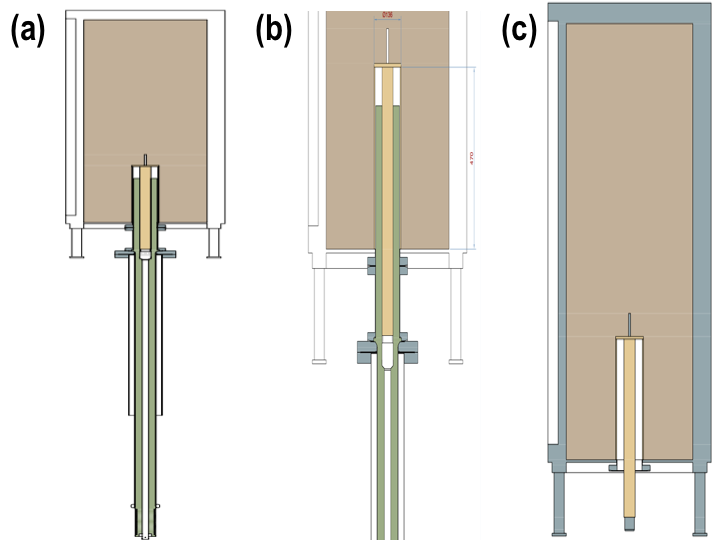
\includegraphics[width=0.5\textwidth]{DP_HVS_dp-hvps-750kv.png}
\end{dunefigure}

%\fixme{I added hdpe, hvps to glossary. Authors need to define them there please! anne}

Typical Heinzinger power supplies have ripples in the range of $\sim$\SI{30}{k\hertz} with an amplitude of \SI{0.001}{\%V_{nom}} $\pm$ \SI{50}{mV}. A low-pass \dword{r-c} filter designed to reduce the voltage ripple could be integrated into the output of the power supply.  Please note, however, that the required ripple suppression need not be as high as for the \dword{spmod} because the \dune \dword{dpmod} has more effective shielding of the anodic structure, performed by the extraction grid and by the \dword{crp} signal amplification stage. 

%Assuming the distance between the power supply and the cathode to be \SI{15}{\m} and the capacitance of the \fdth and \dword{hv} extender to be about \SI{100}{\pF/\m}, a resistance of a few M$\Omega$ integrated at the output of the power supply is sufficient for noise reduction.

The \dword{hv} \fdth is based on the same successful \dword{icarus} design adopted in both \dword{pdsp} and \dword{pddp}.  In this design, the voltage is transmitted along a stainless steel center conductor on the warm exterior of the cryostat where this conductor mates with a cable end.  Inside the cryostat, the end of the center conductor has a spring-loaded tip that  contacts a receptacle cup mounted on the top of the \dword{hv} extender,
 which is connected to the cathode plane \SI{12}{m} below. The center conductor of the \fdth is surrounded by \dword{uhmwpe}.  

To first order, the upper bound of operating voltage on a \fdth is set by the maximum \efield on the \fdth.  Increasing the insulator radius reduces the \efield.  For the target voltage, the \fdth uses a \dword{uhmwpe} cylinder of at least \SI{15.2}{\cm} (\SI{6}\,in) diameter.  In the gas space and into at least \SI{15.2}{\cm} of the liquid, a tight-fitting stainless steel ground tube surrounds the insulator.  The ground tube has a Conflat\footnote{Conflat\texttrademark{}, \url{https://www.lesker.com/newweb/flanges/flanges_technicalnotes_conflat_1.cfm}.} flange of at least \SI{25.4}{\cm} (\SI{10}\,in) in diameter welded onto the cryostat.

A prototype \fdth \footnote{The prototype was manufactured by the company CINEL\texttrademark{} Strumenti Scientifici Srl.}  has been successfully tested up to \SI{-300}{\kV} in pure argon in a dedicated set up; two similar prototypes are %being 
installed in \dword{pdsp} and \dword{pddp}.

%%%%%%%%%%%%%%%%%%%%%%%%%%%%%%%%%%%%%%%%%
\subsection{High Voltage Extender and Voltage Degrader}

The \dword{hv} must be guided from the top of the cryostat to the cathode (\SI{12}{\m} below the \dword{lar} surface), so an extension of the \dword{hv} \fdth is required, as shown in Figure~\ref{fig:dp-hvft-extender} a, b, and c. The extender contains an inner conductor at \dptargetdriftvoltneg surrounded by an insulator. The extension runs the entire height of the drift volume, so metallic rings (degrader rings) are installed on the periphery of the extension close to the field-shaping ring. Each degrader ring is electrically connected to the field-shaping ring at the same height, thus guaranteeing that the drift field in the \dword{lar} between the extender and the \dword{fc} remains undistorted. An alternative, equipping the extender with an independent voltage degrader, is being evaluated. This alternative could eliminate the large %amount 
number of connecting strips on the \dword{fc} profiles; on the other hand,  it requires an independent path to ground.


\begin{dunefigure}[\dual HV \fdth and extender]{fig:dp-hvft-extender}{Sketches of \dword{hv} \fdth and \dword{hv} extender-degrader: (a) Overview of the \dword{hv} \fdth, \dword{hv} extender, and degrader chain; (b) details of the top portion of the \dword{hv} extender and its connections to the field-shaping rings; (c) details of the \dword{hv} extender and degrader connection to the bottom part of the \dword{fc}, including the connection to the cathode plane.}
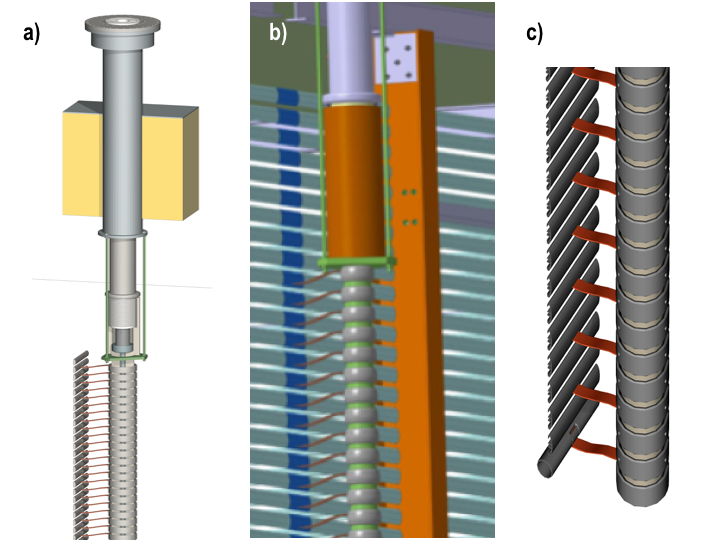
\includegraphics[width=0.75\textwidth]{DP_HVS_dp-hvft-extender.png}
\end{dunefigure}

%%%%%%%%%%%%%%%%%%%%%%%%%%%%
%\subsection{Cathode Plane and Ground Grid - 3 pages}

\subsection{Cathode Plane}
\label{sec:dp-hv-system-cathode}

The \dune \dpmod{}'s cathode plane forms the  bottom of the \dptpcwdth (W) $\times$ \tpcheight (H) $\times$ \dptpclen
% \SI{12}{\m} (W) $\times$ \SI{12}{\m} (H) $\times$ \SI{60}{\m} (L) 
drift volume and provides a constant potential surface at \dptargetdriftvoltneg{}. It receives its \dword{hv} from the central conductor of the \dword{hv} extender that carries the voltage from the power supply through the \dword{hv} \fdth.  

The cathode plane consists of fifteen adjacent \SI{4}{\m} $\times$ \SI{12}{\m}  modules to cover the \SI{60}{\m} length of the \dune \dword{dp} \dword{tpc}. 
The cathode module design is based on the design used in \dword{pddp}, with modifications to %reach 
accommodate the \SI{12}{\m} span of the \dune \dword{dpmod} and implement features to electrically segment the cathode plane.

As Figure~\ref{fig:dune-dp-cathode} shows, each cathode module is constructed from two \SI{12}{\m} long trusses made from thin-walled stainless steel tubes with approximately \SI{50}{\mm} outer diameters.  They can either be prefabricated and transported underground like the large cryostat beams or assembled in the underground cleanroom from sectional parts. 
%\fixme{The DP IIC chapter should address this. Anne}
The trusses are \SI{2}{\m} apart and are %inter
connected at both ends %by two 
to stainless steel tubes (outer tubes in the figure) that %serve as the outer edges of the cathode plane under the \dword{fc}. 
run under the \dword{fc} and form the outer tube ring of \SI{144}{\m} surrounding the cathode plane.

\begin{dunefigure}[A view of a ProtoDUNE-DP cathode module]{fig:dune-dp-cathode}
{A view of a \dword{pddp} cathode module:  Construction uses a pair of stainless steel trusses as the framework with an array of coated \dword{frp} rods. % with resistive surfaces. 
The lower-left inset shows the details of the resistive interconnect and the lifting tab on the cathode truss structure. The upper-right inset is a detailed view of the components in a resistive union (Credit: BNL).}
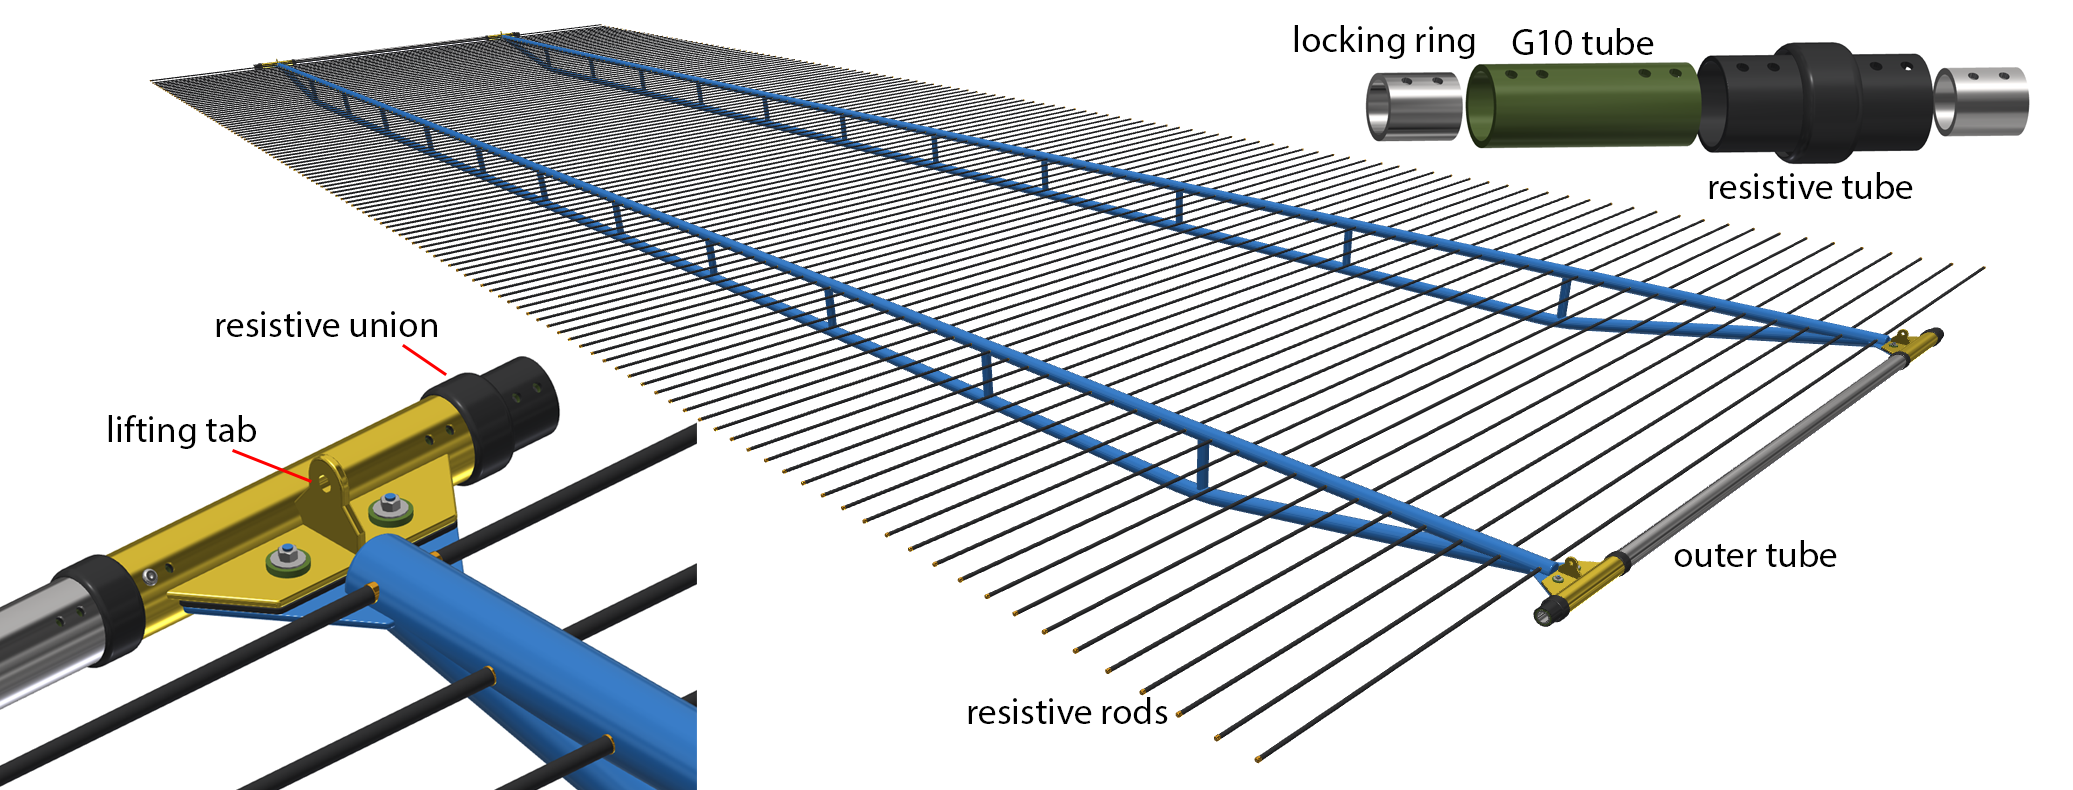
\includegraphics[width=0.9\textwidth]{DP_HVS_cathode_module.png}
\end{dunefigure}

A total of \num{122} resistive rods, each \SI{10}{\mm} in diameter, are installed at a  \SI{10}{\cm} pitch through %\fixme{holes in?} 
the holes in the %long 
straight upper tubes of the trusses, forming the effective cathode plane. The rods are made from extruded \dword{frp} and wrapped with a layer of the resistive DuPont Kapton XC film \footnote{http://www.dupont.com/content/dam/dupont/products-and-services/membranes-and-films/polyimde-films/documents/DEC-Kapton-summary-of-properties.pdf}, also used in the \dword{sp} \dwords{cpa}. %These resistive rods 
They have metal end caps to smooth out the sharp edges of the exposed resistive film and metal sleeves where they cross the trusses, so they can be locked down to the trusses with screws.  %the long upper tube of 
 
%\fixme{Anne to fix - footnote for dupont kapton}

Preliminary mechanical analysis of the design shows that the deflection of the structure is approximately \SI{4}{\cm} when warm and roughly \num{60}\% of that when in \dword{lar} (Figure~\ref{fig:dune-dp-cathode-deflection}). The cathode modules are suspended %to the matching 
from the corresponding \dword{frp} I-beams on the \dword{fc} super-modules along the two long %walls of the cryostat
sides of the \dword{detmodule}. %The resistive coupling between trusses and modules is achieved by custom resistive unions as shown bottom left inset of Figure~\ref{fig:dune-dp-cathode}. 
Custom resistive unions, shown in the bottom left inset of Figure~\ref{fig:dune-dp-cathode}, provide the coupling between trusses and %\fixme{ CPA modules? looks like it should be outer tubes} 
\dword{fc} modules. Each is made from a resistive sleeve, a G10/FR4 stiffening tube, and two locking rings, as depicted in Figure~\ref{fig:dune-dp-cathode}, top-right inset. 

\begin{dunefigure}[Deflection of the cathode truss]{fig:dune-dp-cathode-deflection}
{Finite element analysis (FEA) of the cathode truss showing the deflection of the structure under its own weight and half the weight of the \dword{frp} resistive rods at room temperature.  The deflection should reduce to approximately 60\% once the structure is submerged in \dword{lar}  (Credit: BNL).}
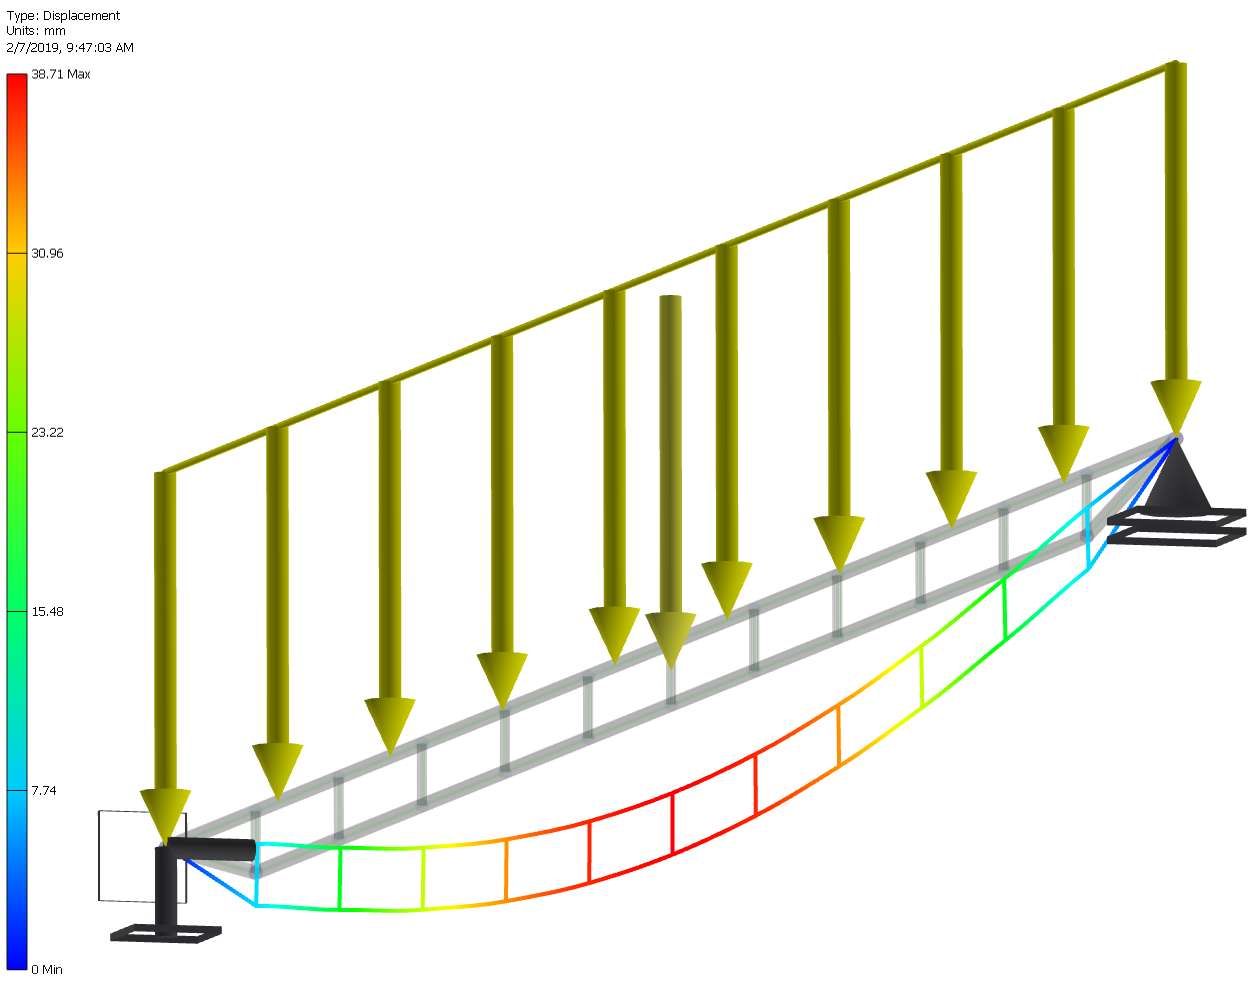
\includegraphics[width=0.7\textwidth]{DP_HVS_cathode_frame_FEA.png}
\end{dunefigure}

An \dword{hv} bus, made from \dword{hv} cable segments, is threaded through the outer tube ring, which is formed once the full set of cathode modules are in place, to form a conductive ring that distributes the cathode bias voltage.  The mounting plates (shown in gold in Figure~\ref{fig:dune-dp-cathode}) at both ends of a cathode truss are directly connected to the \dword{hv} bus via metal rings inside the tube.  These mounting plates are also connected to the \dword{fc} resistive divider chains. Between the mounting plate and the %cyan colored 
truss, a layer of resistive sheet provides an additional barrier to energy transfer.  The resistivity of this sheet will be chosen to ensure the ionization current from \Ar39 activity 
%\fixme{activity?} 
and the ion feedback from the \dword{lem} multiplication will not cause significant voltage drop on the cathode.

The energy stored in the volume between the cathode plane and the \dword{gg} (described in Section~\ref{sec:dp-hv-groundgrid}),
%\fixme{can we just use \dword{gg} like the SP mod? the general definition is the same. anne}
which sits under the cathode and above the \dwords{pd}, is estimated at %approximately 
\SI{1.7}{\kilo\joule} 
over the \dptpcwdth $\times$ \dptpclen area based on the cathode voltage and the distance (\SI{1}{\m}) between the cathode and the \dword{gg}. 
%A sudden discharge from the cathode to the cryostat membrane could cause severe damage to both.  ------Anne rewording to emphasize safety ---
The modular construction of the cathode minimizes potential damage to either or both components in case of a sudden discharge from the cathode to the cryostat membrane.
%The modular construction of the cathode helps minimize this effect in case of discharge. The cathode plane's structural elements (trusses) are metallic, spanning the 12m width of the TPC.  However, in the 60m direction, 
Along the \SI{60}{m} length of the \dune \dword{dpmod}, the trusses and their interconnecting metal tubes are %all 
coupled with highly resistive unions (approximately \si{\giga\ohm}) %.  The resistive elements are 
designed to restrict the flow of current from %the 
any potential discharge site.    
%%During assembly in the cryostat, the cathode units are kept electrically insulated. Each unit is then connected to their immediately adjacent neighbors through resistive tubular elements with value of the order of the \si{\giga\ohm}  
%\fixme{JY to Bo and Francesco: I have no idea what this particular sentence is trying to say.  If the neighboring cathode planes are connected through a \si{\giga\ohm} resisters - one or two? and how? - they are not insulated from each other.  Is this trying to say that the cathode units are connected with each other only through these resisters that connects the frames?  Don't we need some description as to how we envision doing this?  The description for this inter-cathode unit module connected is quite imbalanced compared to the structure of each unit.} 

%Dividing the \SI{1.7}{\kilo\joule} of energy evenly among the \num{15} cathode modules, each has about \SI{110}{\joule}.  On a cathode module, each truss has about 1/8 of this energy, while the resistive rods share the remaining 3/4. A worst case discharge is from a cathode truss, where $\sim$\SI{15}{\joule} is directly available to contribute, and the rest of the \SI{95}{\joule} arrives with a few milliseconds time constant.  The energy transfer from other cathode and field cage modules must pass through \si{\giga\ohm} of resistive connections and therefore will have time constants of the order of a second.
Assuming that the \SI{1.7}{\kilo\joule} of energy is stored evenly among the \num{15} cathode modules, each stores approximately \SI{110}{\joule}.  On a cathode module, each truss stores about an eighth of this energy (one quarter in total), while the resistive rods share the remaining three quarters. %\fixme{and the last eighth?} 
A worst-case discharge would come from a cathode truss, where $\sim$\SI{15}{\joule} is directly available to contribute with the remaining \SI{95}{\joule} arriving within a time constant of a few milliseconds.  The energy transfer from other cathode and \dword{fc} modules must pass through \si{\giga\ohm}s of resistive connections and therefore will have time constants of approximately one second.

%% Given the \SI{100}{\pico\farad} capacitance of each cathode unit \fixme{JY to Bo and Francesco: I calculate 396pF as the minimum not 100PF.}, any discharge occurring in one unit will release at most 
%% \SI{21}{\joule} of stored energy \fixme{JY to Bo and Francesco: I calculate 72J minimum.  Can we get these numbers finalized?}
%% while the discharge rate to the other units is slowed to the several-hundred-millisecond range.

\begin{dunefigure}[ProtoDUNE-DP cathode field]{fig:dune-dp-cathode-field}
{Electrostatic calculation of the surface \efield on a section of the cathode (upper) and \dword{gg} (lower) structures. The outer tube and the bottom tube of the cathode structure have high surface \efield. The maximum \efield is approximately \SI{30}{\kV/\cm} at the curved section of the bottom tube (Credit: BNL).} 
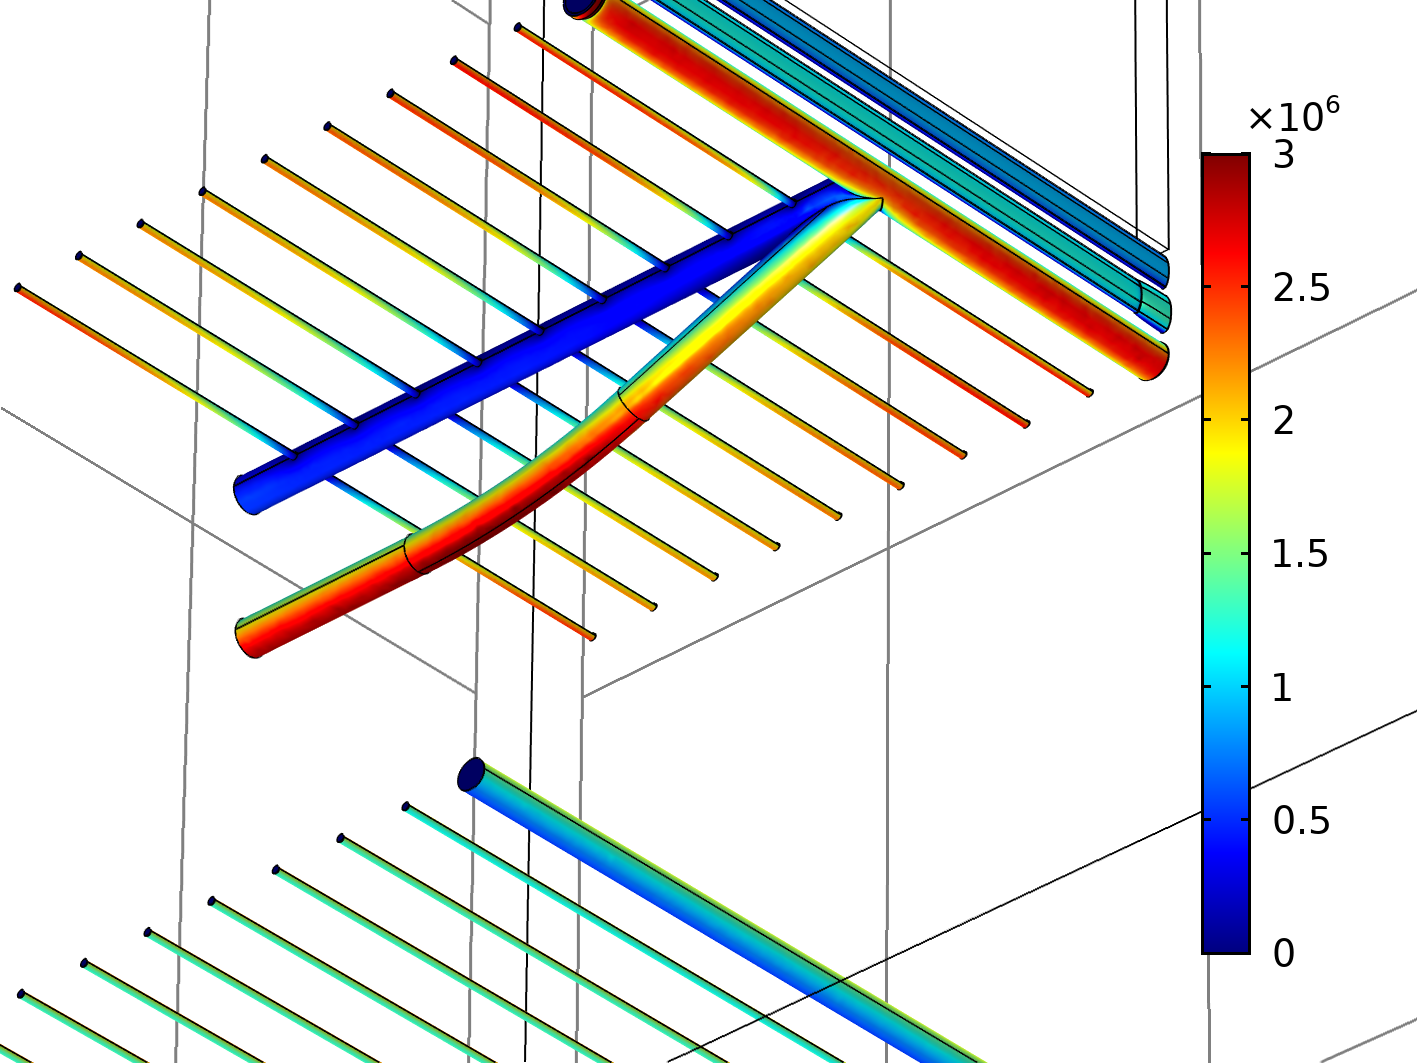
\includegraphics[width=0.7\textwidth]{DP_HVS_cathode_E_field2.png}
\end{dunefigure}

Detailed calculations are in progress to determine the final shape and the size of the cathode and \dword{gg} frames to %meet the requirement that 
limit the maximum \efield to \SI{30}{\kV\per\cm}  
throughout the \dword{lar} volume (Figure~\ref{fig:dune-dp-cathode-field}; see %Requirement 2 in 
Table~\ref{tab:specs:DP-HV}) and to correct the non-uniformity of drift field at the edges of the cathode (see Figure~\ref{fig:dune-dp-cathode-field-2D}).  Structural calculations must also verify the planarity of the cathode as it hangs on the \dword{fc} supports.
Values and voltage characteristics of the connecting resistors will also be defined based on the results of dedicated simulations of the cathode electrical model.

\begin{dunefigure}[ProtoDUNE-DP cathode field \twod]{fig:dune-dp-cathode-field-2D}
{Looking along the beam direction, \twod plot of the \efield (color gradient), equipotential contours (black), and electric field lines (gray) in one half of a \dword{tpc}. The right vertical edge is a symmetry plane. The \efield unit is in Log$_{10}\,$(V/m).  (Credit: BNL).} 
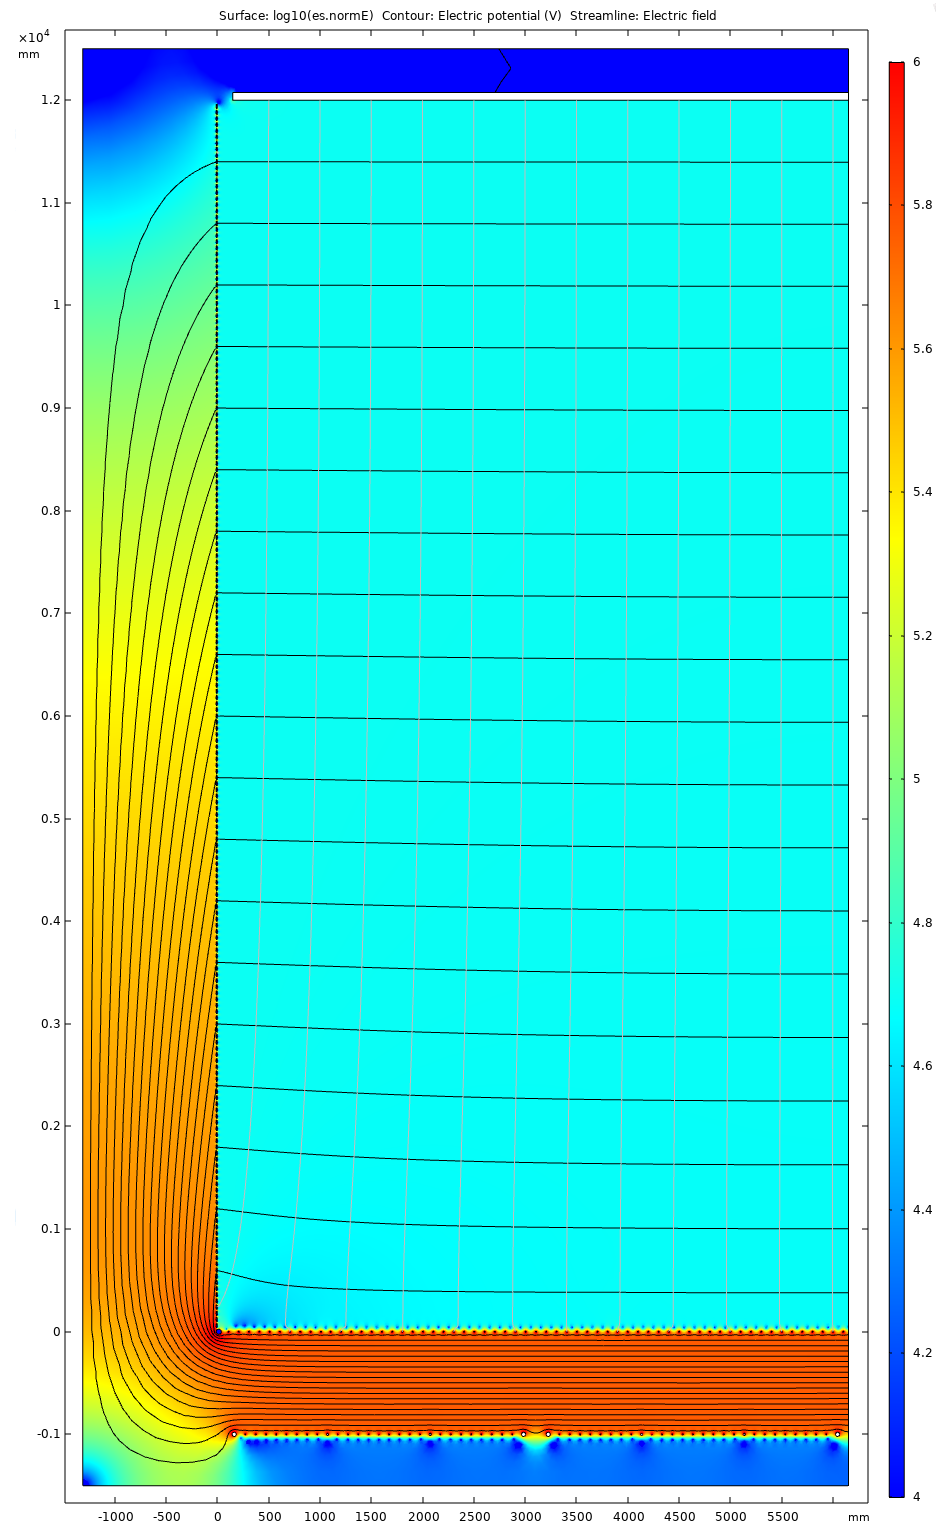
\includegraphics[width=0.42\textheight]{DP_HVS_cathode_E_field_2D.png}
\end{dunefigure}

\subsection{Ground Grid}
\label{sec:dp-hv-groundgrid}

An array of \dword{gg} modules %\fixme{JY: We should define the dimension of GG unit.  AH: agreed!! 2.72 m square? with gap between gg's of 3.06-2.72=.34m? This doesn't seem right... the next paragraph is unclear.} 
is installed above the \dwords{pmt} and below the cathode plane to provide a low \efield environment for the \dwords{pmt} and shield them from a potential %\fixme{a potential?} 
\dword{hv} discharge from the cathode plane.

A \dword{gg}  module, shown in Figure~\ref{fig:dp-hv-ground-grid}, is made from  stainless steel (\dword{aisi} Type 304) tubes 
%\fixme{JY: Where does this number come from? Is this actually true?  I cannot count 304 in the figure. AH: 304 appears to be a grade of SS.}.  
and %covers 
sits above a \num{3} $\times$ \num{3} array of \dwords{pmt} at \SI{1.02}{\m} pitch. The \dword{gg} modules are placed on the cryostat floor at a pitch of \SI{3.06}{\m}. The \num{4} legs for each \dword{gg} module are \SI{2.72}{\m} apart, taking into account the \SI{0.34}{\m} pitch of the membrane corrugation, so the feet are always on the flat part of the membrane. To avoid damage to the membrane floor, the feet will be covered with a Teflon 
sheet, which will %make the \dword{gg} unit modules 
electrically isolate them from the membrane cryostat. The modules are not physically in contact with each other %which means they 
and can be individually read out, if needed, to monitor \dword{hv} stability. %In this case, proper grounding of the ground grid modules will be ensured through the grid read-out boards. \fixme{readout boards not yet defined. anne}
%
%\fixme{JY: But they are in electrical contact with teach other through the ground on the cryostat floor.  So how would you envision reading them out individually unless the legs are electrically isolated from the GG plane?}. 
%
Otherwise, electrical contact to the membrane (detector ground) will be through the legs via springs that penetrate the Teflon sheets % to the four legs, 
or by grounding wires %\fixme{from there?} 
on the edges of the cryostat. To cover the entire area of the cathode, a total of \num{80} \dword{gg} modules are arranged in %the form of 
a \num{4} $\times$ \num{20} array. Preliminary analysis of the \dword{gg} structure %shows we can expect 
indicates approximately \SI{1}{\cm} of sag in the center of %the 
a unit grid. Detailed studies of the grid geometry are ongoing to ensure that the requirement for the maximum local field is satisfied. Figure~\ref{fig:dune-dp-cathode-field} shows the surface \efield on the cathode and \dword{gg} near the  %\fixme{the?} 
cathode edge. The maximum \efield is under the curved section of the lower truss member at the \SI{30}{\kV/\cm} limit.

\begin{dunefigure}[A single ground grid module]{fig:dp-hv-ground-grid}
{Left: A view of a \dword{gg} module; Right: \dword{gg} position relative to the membrane corrugation and \dword{pmt} locations (Credit BNL).}
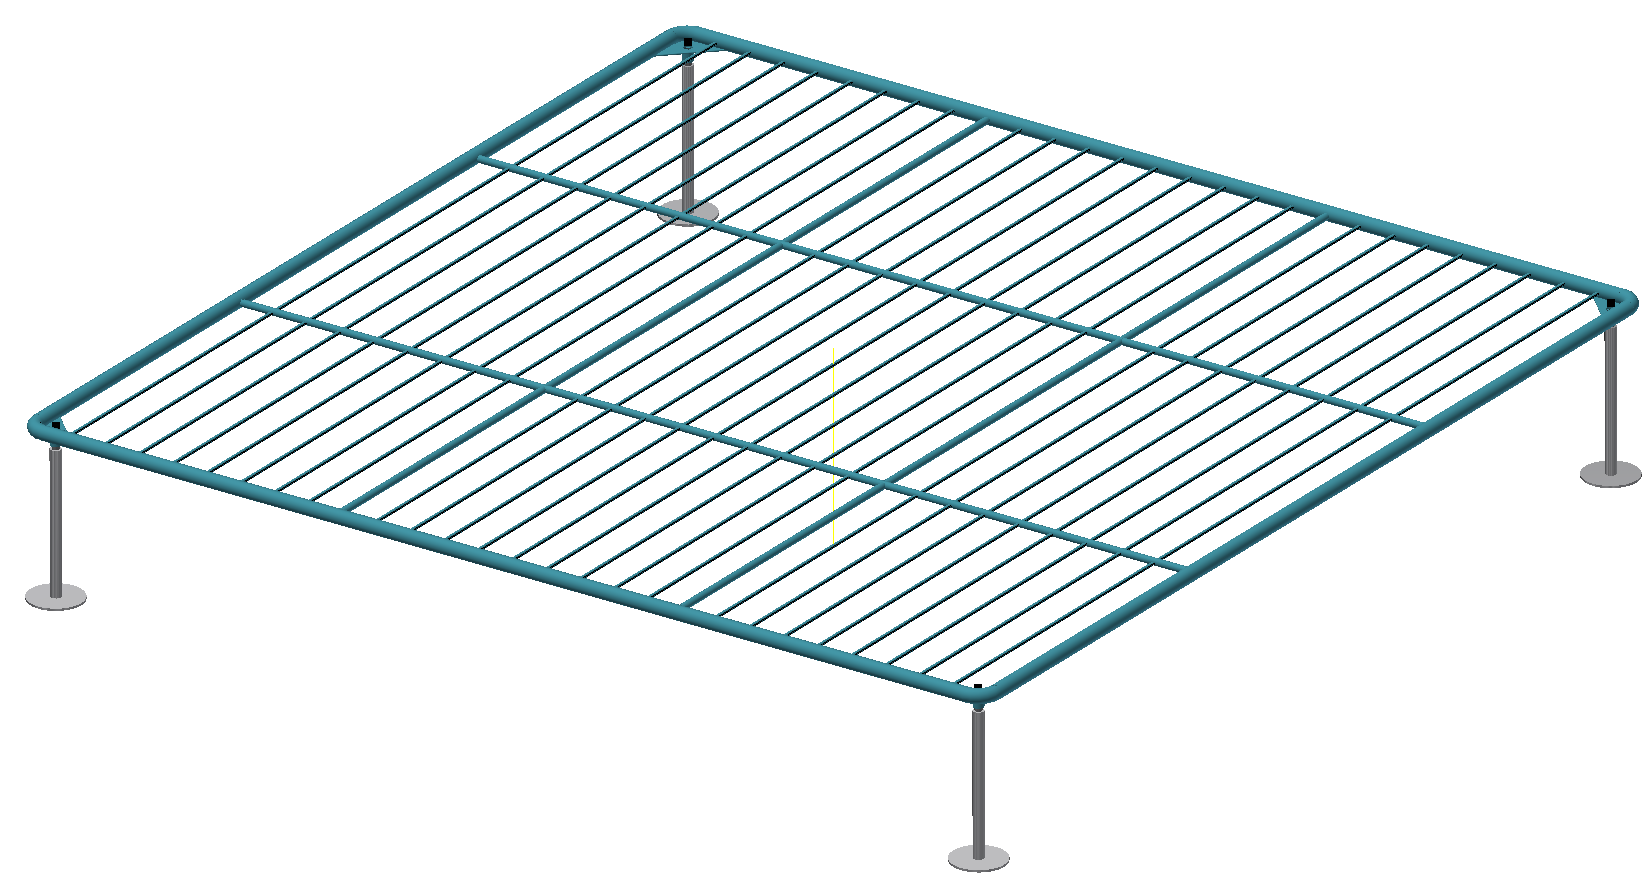
\includegraphics[width=0.6\textwidth]{DP_HVS_ground_grid_3x3.png}
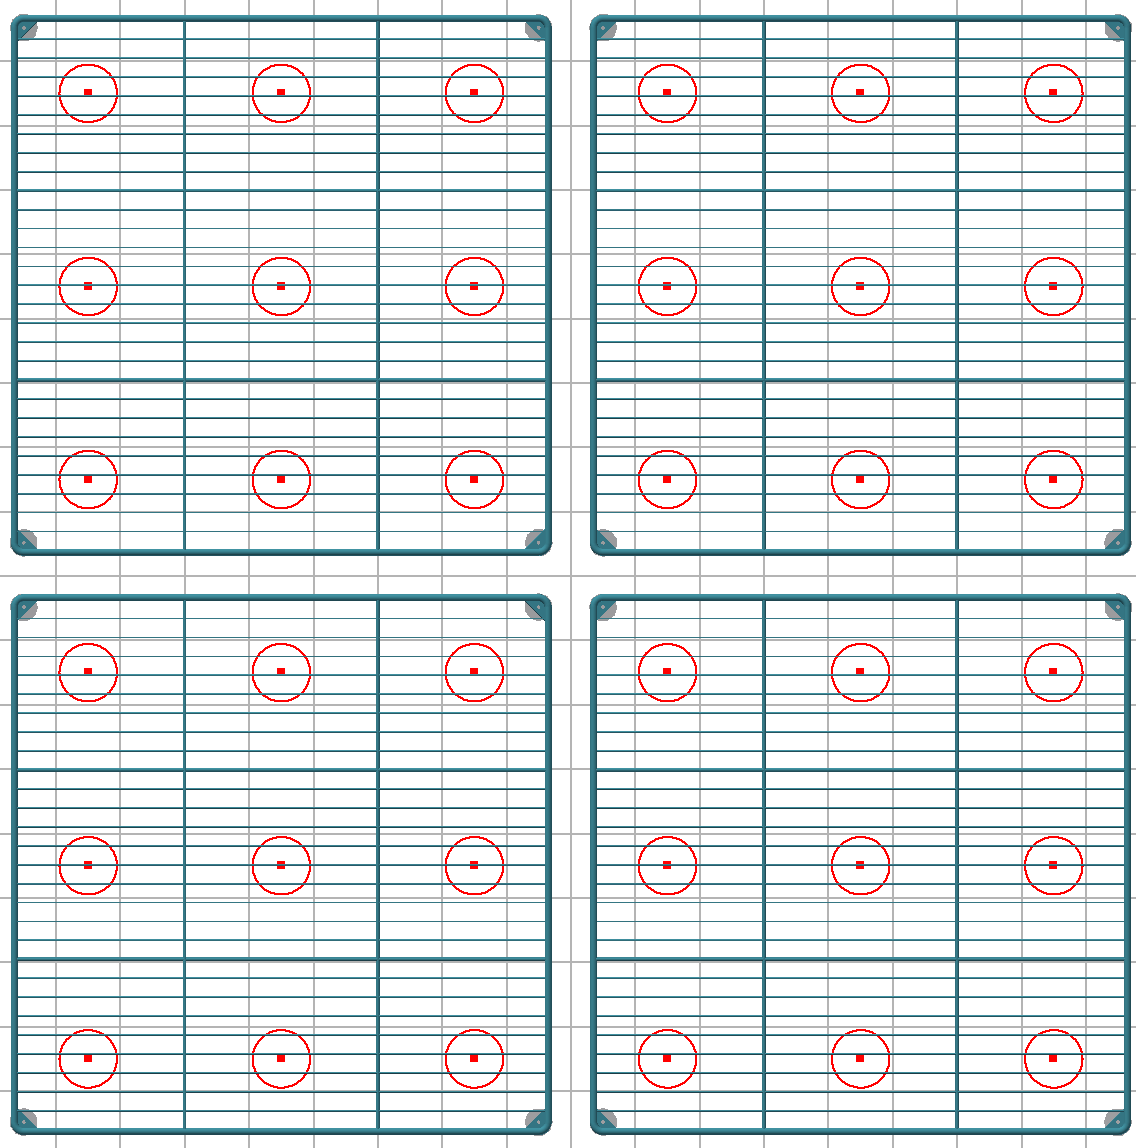
\includegraphics[width=0.3\textwidth]{DP_HVS_ground_grid_plan_view.png}
\end{dunefigure}


\subsection{Field Cage}
\label{sec:dp-hv-system-fc}


Like the \dune \dword{sp} \dword{fc}, the \dune \dword{dp} \dword{fc} is modular; it is broken down into super-modules, modules, and submodules, as listed in Table~\ref{tab:hvcomponents}.  The \efield must be vertical, so the \dword{fc}'s equipotenial conductors, the field-shaping rings, run horizontally around the perimeter of the active volume. The conductors are extruded aluminum open profiles. %These rings are formed by connecting together \dword{fc} modules that contain the extruded aluminum open profiles that are sections of the rings. 

Profile sections are arranged into \dword{fc} submodules.
%are electrically connected by resistive elements to form the full \SI{144}{m}-long equipotential rings that run the full perimeter of the drift volume. 
An \dword{fc} submodule is \SI{2}{\m} high and \SI{4}{\m} wide. %\fixme{and has how many profiles in it?}
 Six submodules stack vertically to make a full \SI{12}{\m} high module. Three adjacent modules form a super-module. One row of \dwords{hvdb} mounts to each end of the middle module's profiles. On each side of the middle module, a \SI{1}{\giga\ohm} resistive sheath, a \SI{12}{\cm} long tube in the shape of the profile, connects each profile with its same-height counterpart in the side module. Surge suppressing varistors are connected in parallel to protect the resistors. Similar resistive interconnects are made between pairs of  profiles of adjacent super-modules to provide more redundancy in the \dword{fc} electrical connection, leveraging the row of \dwords{hvdb} in the neighboring super-modules.  The connected profiles reach the same bias voltage because no current flows along the ring that they form.  %\fixme{it seems like each end would need its own row of HVDB. I must misunderstand something. Anne}

Profiles at the same height in adjacent modules are interconnected horizontally through resistive sheaths. All same-height profiles form a closed, electrically continuous rectangular ring. 
The four walls surrounding the \dword{tpc}'s active volume are formed using \num{199} of these rings stacked vertically in \SI{6}{\cm} pitch. The aluminum profiles are attached to I-beams made of pultruded \dword{frp}. %\fixme{are these structural elements the "columns"?} 
%\fixme{This abbreviation is used frequently in this chapter, but it is not in the common glossary. It probably should be.}

\dword{frp} is non-conductive and strong enough to withstand the \dword{fc} loads. %in the temperature range of \SI{-150}{\degreeCelsius} to \SI{23}{\degreeCelsius}.
This material meets the  Class A International Building Code classification for flame spread and smoke development, as characterized by ASTM E84\footnote{\url{https://www.astm.org/DATABASE.CART/HISTORICAL/E84-07.htm}}. 

\begin{dunefigure}[FC elevation]{fig:dune-dp-fc-elevation}
{A side view of one end of the \dword{hv} system components in the \dword{tpc} showing the top frame, left-most super-module with profiles, and the \dword{gg} array on the bottom.  The \endwall super-module on the left is pushed away from the cryostat wall by \SI{0.5}{\m} on the bottom for additional \dword{hv} clearance (Credit: BNL).}
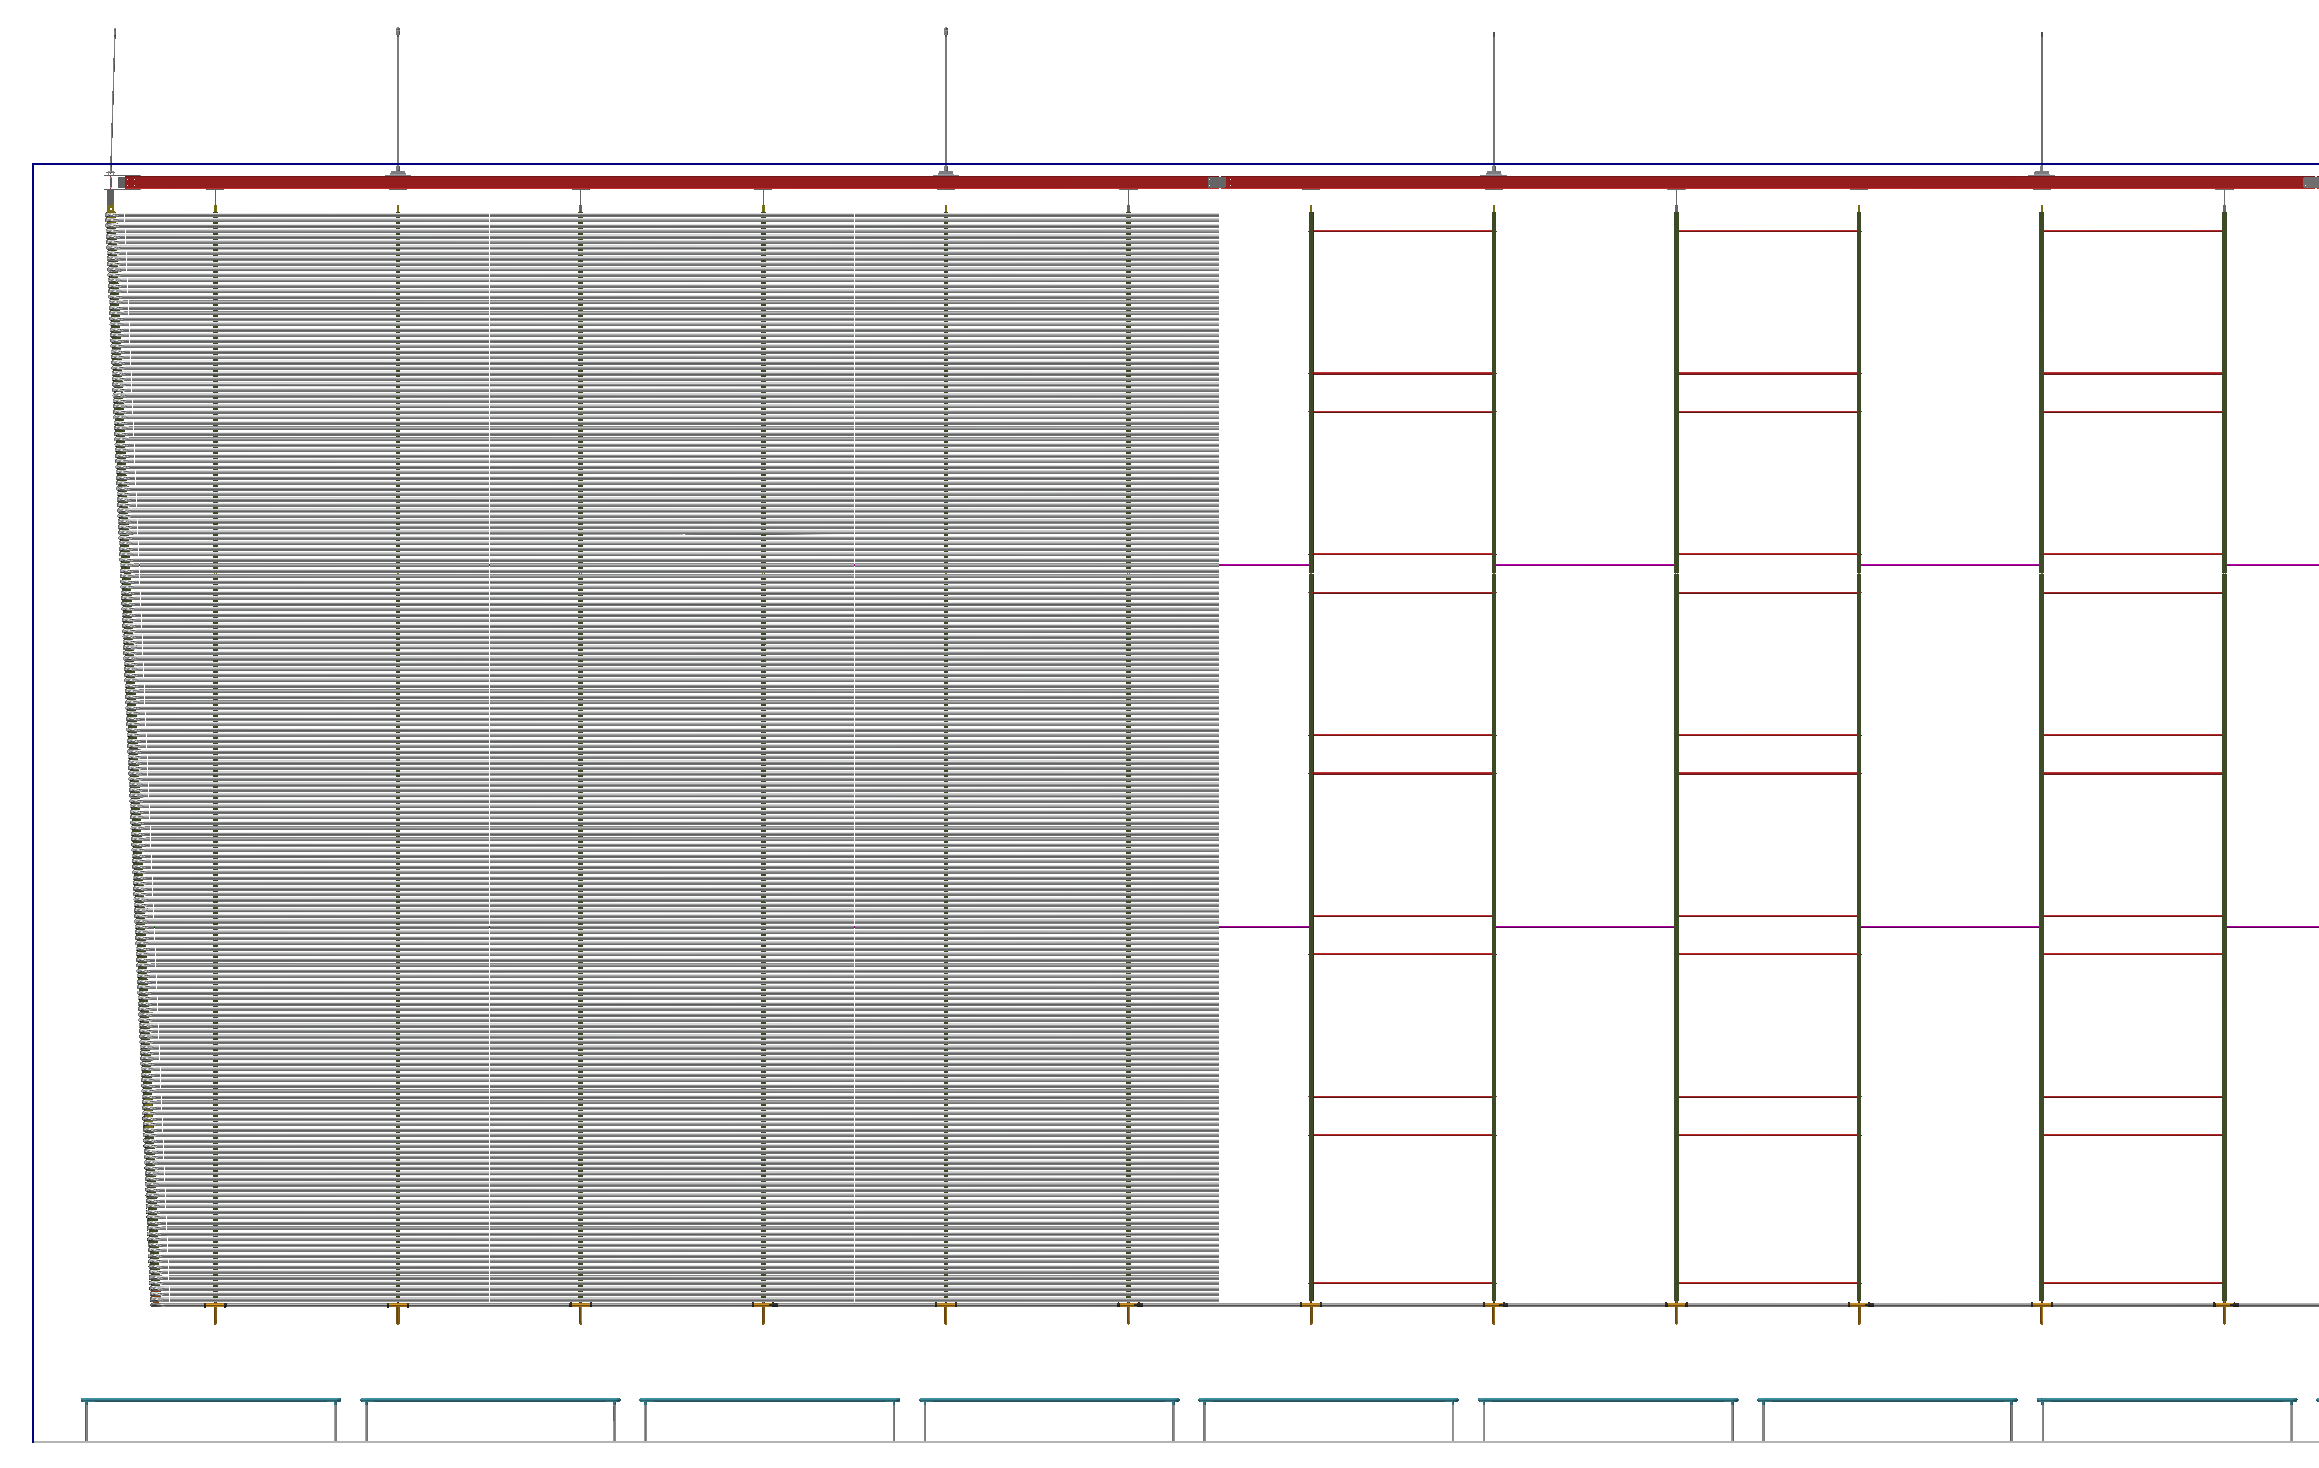
\includegraphics[width=0.9\textwidth]{DP_HVS_FC_elevation.png}
\end{dunefigure}

The entire \dword{fc} is constructed of \num{12} super-modules with the nominal dimensions \SI{12}{\m} wide and \SI{12}{\m} high. Five super-modules run along each long side wall, with one each along the short \endwall{}s.  
The cryostat inner length dimension is \SI{62}{\m}. 
%To gain a safe clearance from the cryostat wall at the bottom of the \dword{tpc} where the cathode is at \dptargetdriftvoltneg, the \endwall \dword{fc} super-modules are designed to be installed \SI{0.5}{\m} from the edge of the active volume. 
%he \endwall super modules are tilted at \num{2.4} degrees with respect to the vertical to allow \SI{0.5}{\m} additional clearance at the bottom of the \dword{fc} where the voltage is at \SI{-600}{\kV}. 
At the top, the inner surfaces of the \dword{fc} profiles are positioned \SI{15}{\cm} away from the \dword{crp}'s active area, which covers \SI{12}{\m}$\times$\SI{60}{\m}, to allow the \dword{fc} support structure to pass through and provide a uniform drift field. 
This leaves only \SI{85}{\cm} clearance between the \dword{fc} \endwall and the cryostat membrane at ground, excluding the cryogenic pipes that protrude further inside the cryostat.

To allow a sufficient safety distance of \SI{1.4}{\m}, which doubles the distance in \dword{pddp}, an additional \SI{50}{\cm} to ground must be added at least to the cathode level, which is at \dptargetdriftvoltneg. 
To avoid any modifications to the \dword{crp}, the top of the \endwall super-modules must stay in place while the bottom must be pulled in by \SI{50}{\cm}, resulting in a tilt of \num{2.4} degrees.
%For the tilted \endwall super-modules, this \SI{15}{\cm} offset applies only to their top edges due to the \num{2.4} degree tilt. 
Figure \ref{fig:dune-dp-fc-elevation} shows a side view of one end of the \dword{hv} system components depicting the \num{2.4} degree tilt.
The side wall super-modules do not need this tilt because the distance between the \dword{fc} and the cryostat wall is \SI{1.5}{\m}.
Each super-module, including its top stainless steel beam, weighs about \SI{1200}{\kg}. 

%copied from earlier section
%The cryostat inner length dimension is \SI{62}{\m}. To gain a safe clearance  from the cryostat wall at the bottom of the \dword{tpc} where the cathode is at \SI{-600}{kV}, the \endwall \dword{fc} super-modules are designed to be installed \SI{0.5}{\m} from the edge of the active volume. The \endwall \dword{fc} will thus be at a \num{2.4} degree angle from vertical.  The bottom parts of the \endwall super-module are tied to the cathode structure to prevent it from swinging back.  Additional braces at 1/3 and 2/3 of the drift depth will support and maintain the \endwall \dword{fc} at this angle.
\begin{dunefigure}[FC submodule view]{fig:dune-dp-fc-module}
{Sketches of an \dword{fc} submodule viewed from inside  (bottom) and outside the the \dword{fc} (top), along with a photograph of a partly completed submodule (bottom-right inset) and a close up photograph of the cross section of a profile attached to the \dword{frp} using a slipnut (top right inset).  The inside view shows the two vertical \dword{frp} I-beams (green) and two horizontal metal cross bars (red) forming the structural framework on which \num{33}  aluminum profiles of length \SI{4}{\m} are attached.  % THESE THINGS AREN'T SHOWN (ANNE) A series of resistive divider boards interconnect all the profiles to provide a linear voltage distribution. The reflector/\dword{wls} panel assemblies of the \dword{pds} will be mounted to the \dword{frp} I-beams with stainless steel screws. 
The outside view shows the outer surface of the \dword{fc} module is insulator-free to avoid \dword{hv} instabilities due to surface charging (Credit: BNL).
}
%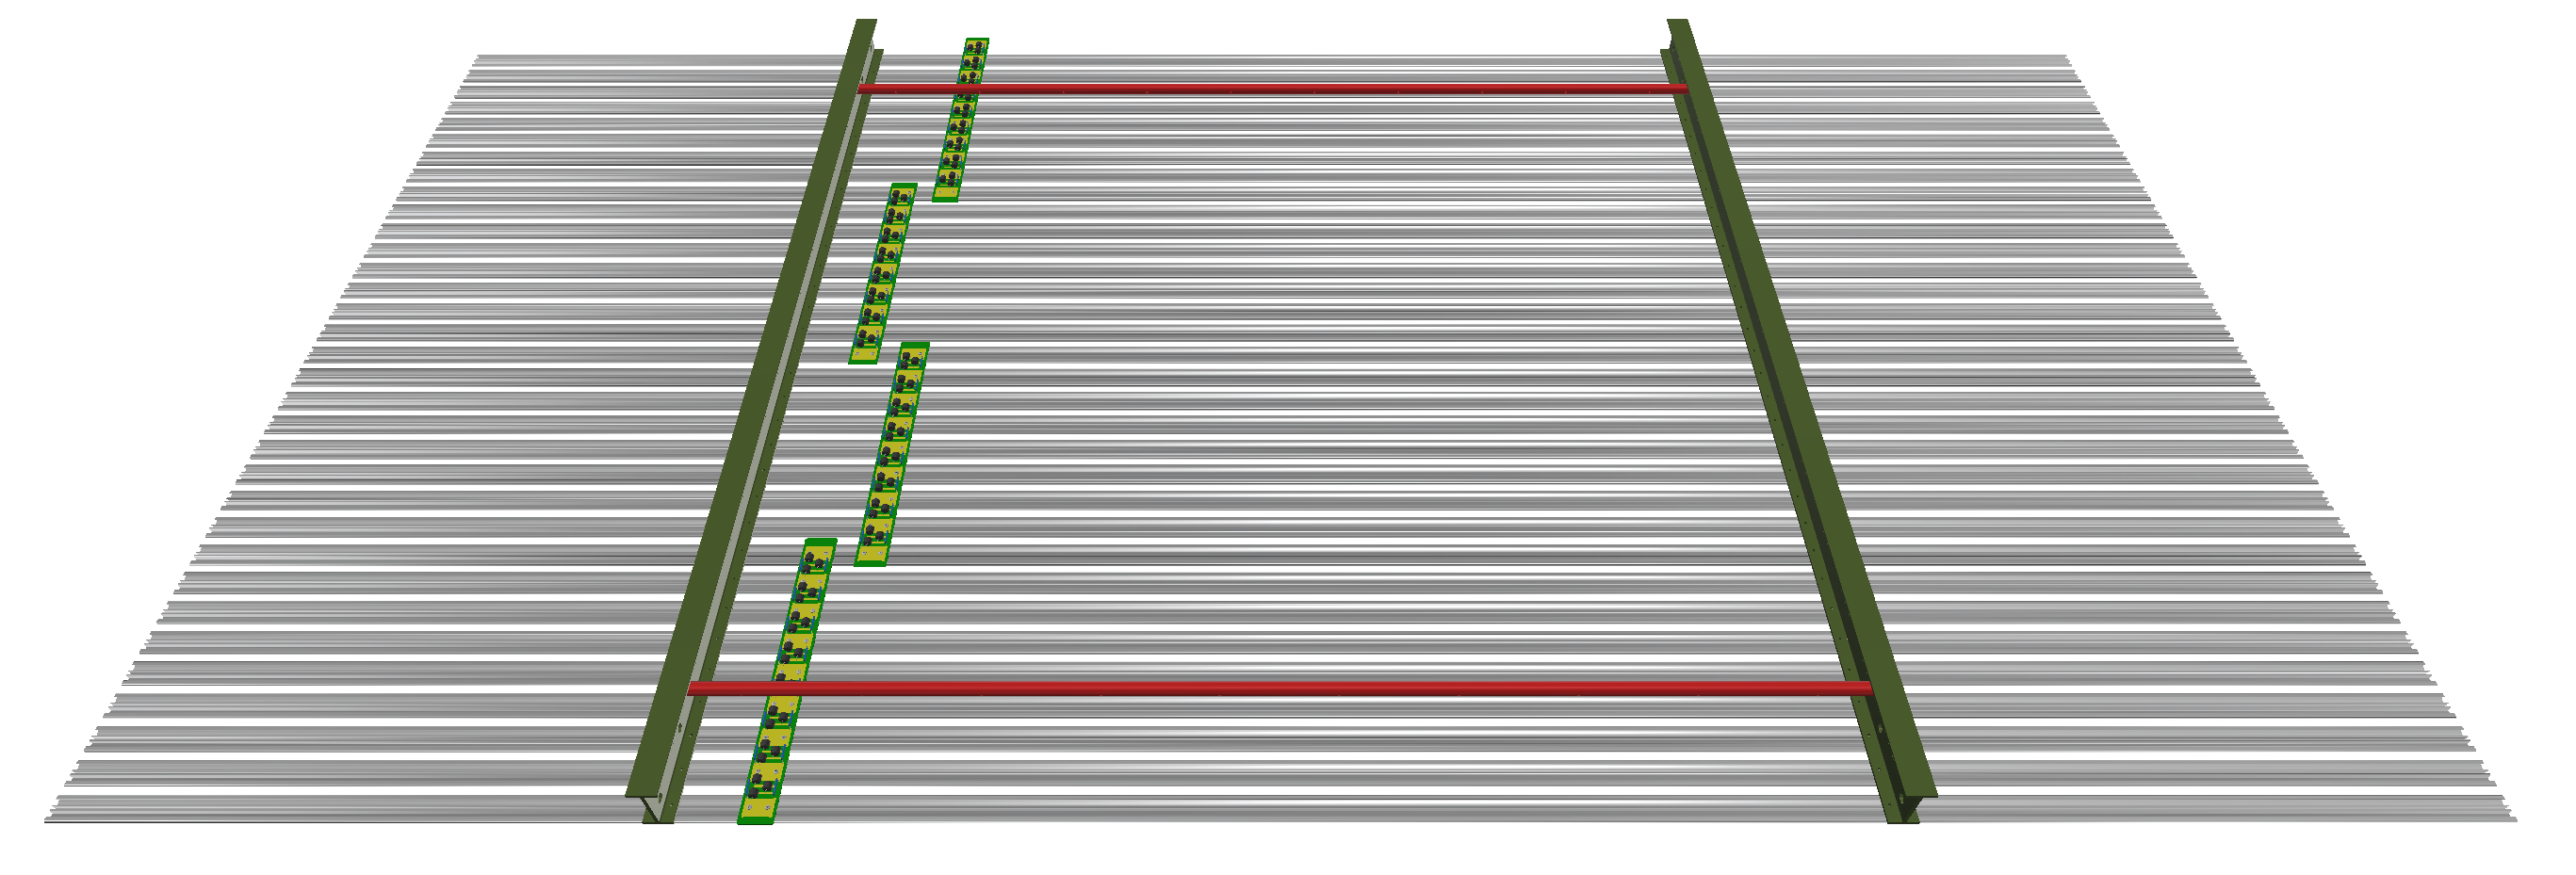
\includegraphics[width=0.9\textwidth]{graphics/DP_HVS_FC_Bottom_Module_Middle.png}
%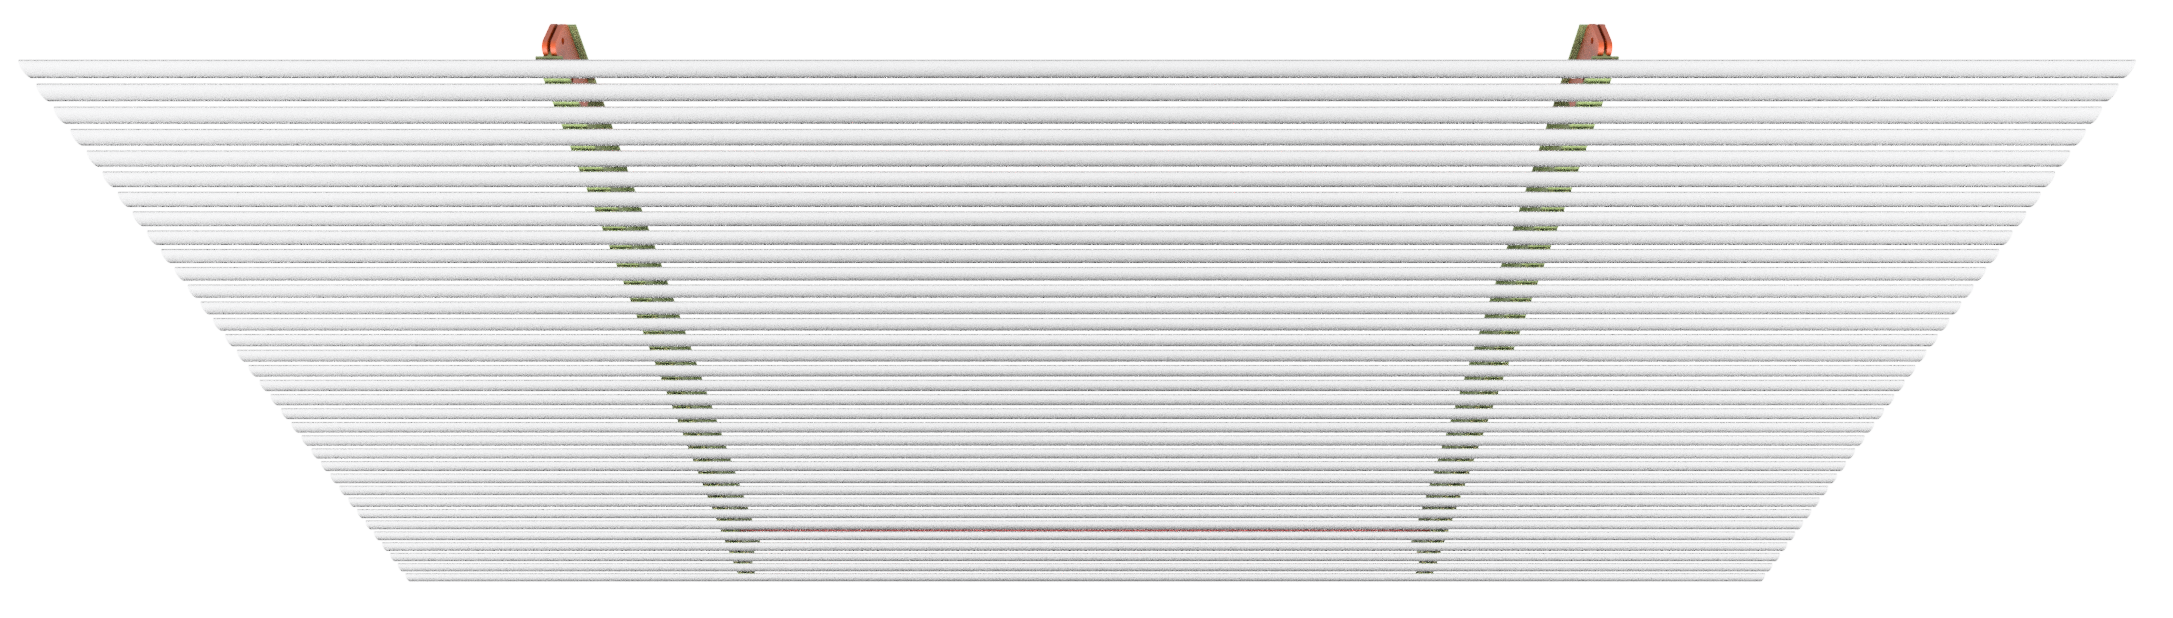
\includegraphics[width=0.9\textwidth]{graphics/DP_HVS__FC_Super_Module_Middle_Outside.png}
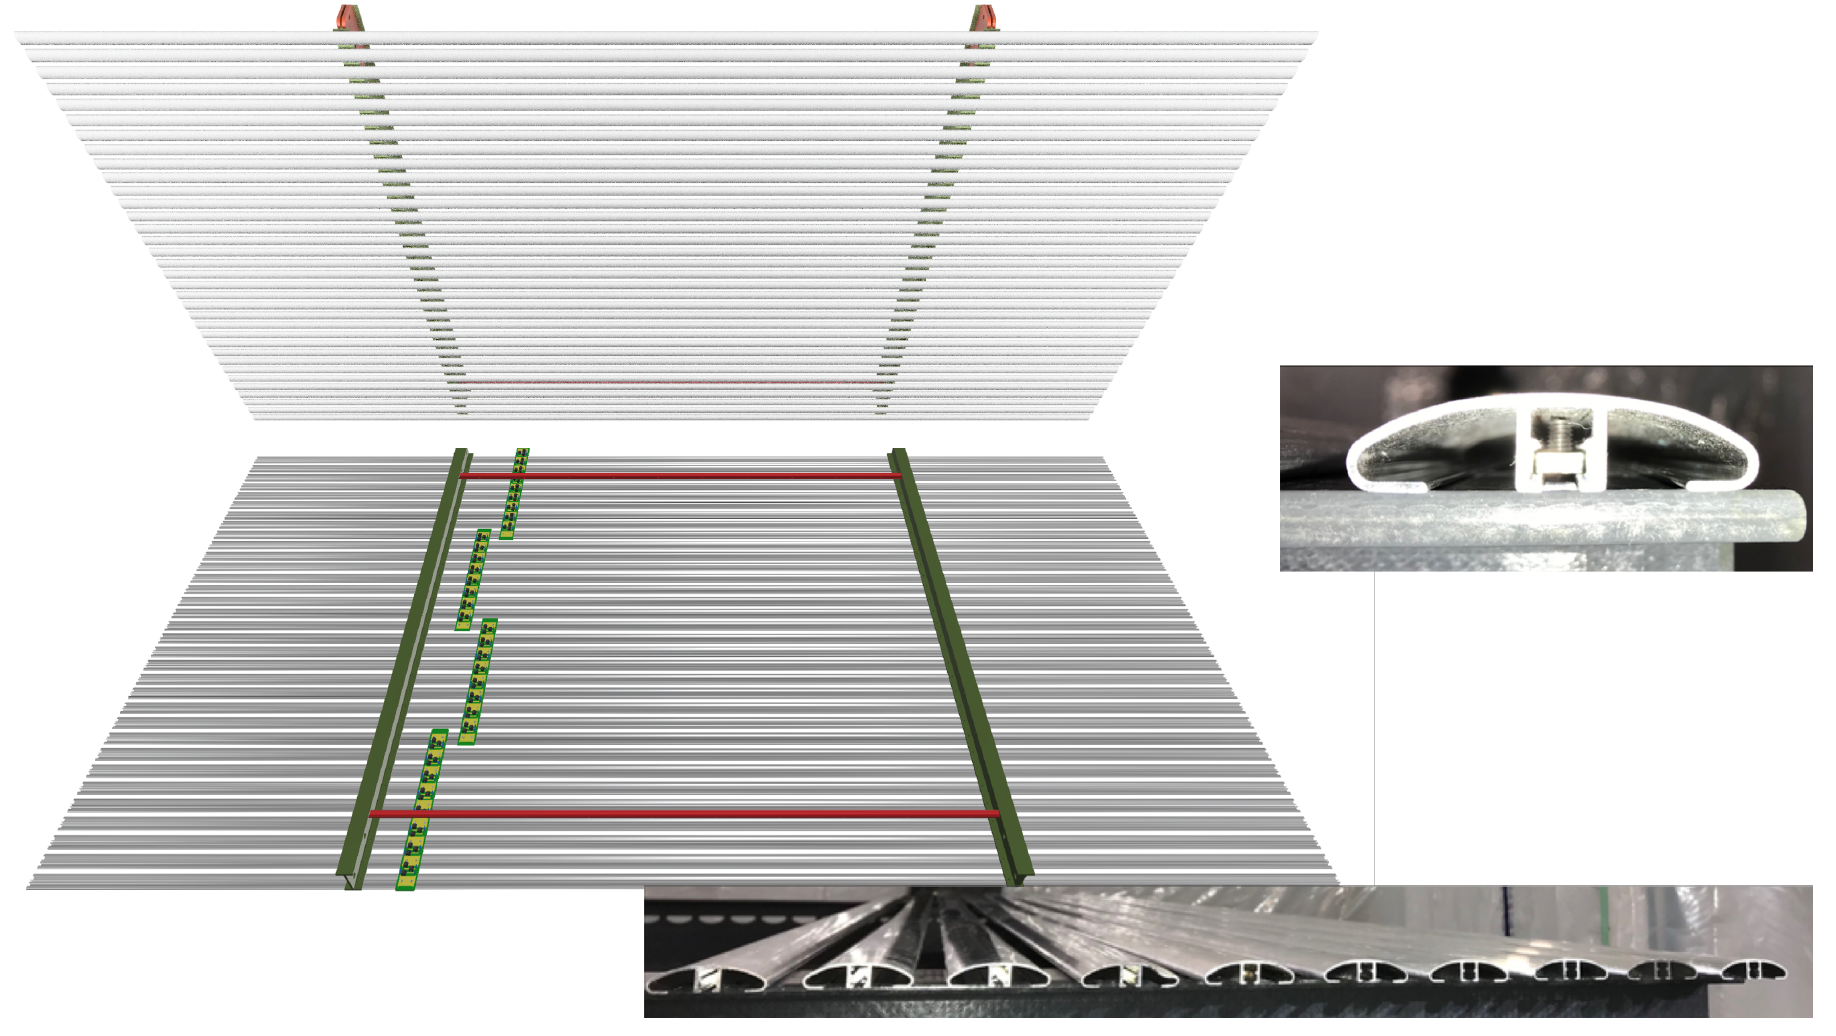
\includegraphics[width=0.9\textwidth]{DP_HVS_FC_Sub_Module.png}
\end{dunefigure}

Each super-module is built from three \SI{4}{\m} (W) $\times$ \SI{12}{m} (H) modules, each of which is made of six \SI{4}{\m} (W) $\times$ $\sim$\SI{2}{m} (H) submodules. All submodules share the same basic construction: two \SI{10}{\cm} (H) $\times$ \SI{5}{\cm} (W) \dword{frp} I-beams with two stainless steel cross bars that form a rigid frame structure (see Figure~\ref{fig:dune-dp-fc-module}). 
Extruded aluminum profiles \SI{4}{\m} long are mounted at a \SI{6}{\cm} pitch on one side of the \dword{frp} I-beams using screws and slip nuts inside the profiles (see the photograph in Figure~\ref{fig:dune-dp-fc-module}, top-right inset). Most of the submodules are \SI{4}{\m} (W) $\times$ \SI{1.98}{\m} (H). Figure~\ref{fig:dune-dp-fc-module} shows the design of a non-corner \dword{fc} submodule. 

%\fixme{add the reflector panels to the table? Is PDS consortium responsible for them? Anne}
The \dword{dp} \dword{pds} has designed \dword{tpb} coated reflector/\dword{wls} panels to be installed on the top half of the \dword{fc} inner surfaces to enhance light collection and improve the \dword{pd} response uniformity throughout the entire %\dword{tpc} 
active volume as described in Section~\ref{sec:dppd-wls}. The dimensions of a reflector/\dword{wls} unit panel assembly to be mounted on the \dword{frp} I-beams of the \dword{fc} submodules are \SI{199}{\cm} (W) $\times$ \SI{186}{\cm} (H). The reflector/\dword{wls} panel assembly at the inter-super-module areas will have special extended assemblies to accommodate the \num{2.4} degree tilt of the end walls: 
 \SI{260}{\cm} (W) $\times$ \SI{186}{\cm} (H) for the corner side wall \dword{fc} submodules %to accommodate the \num{2.4} degree tilt of the end walls, 
 and \SI{290}{\cm} (W) $\times$ \SI{186}{\cm} (H) for all other \dword{fc} submodules at the intersection of two \dword{fc} super-modules. The reflector/\dword{wls} unit module will be mounted on the \dword{frp} I-beams of the \dword{fc} submodules with six screws. The details of the reflector/\dword{wls} panel assembly design can be found in Sections \ref{sec:dppd-wls} and \ref{sec:dp-pds-mechanics}.
 
The extruded aluminum profiles are mounted on the cryostat-wall-side surface of the flange of the \SI{10.2}{\cm} (\SI{4}{in}) \dword{frp} I-beam via two stainless steel screws and aluminum slip nuts in the center enforcement rail of the profile (see  Figure~\ref{fig:dune-dp-fc-module}, bottom-right inset). Each profile is secured fully  on one of the \SI{10.2}{\cm} I-beam flanges and more loosely on the other, sufficient %ly secured 
to hold the profile in place. This prevents stress and distortion resulting from the small \dword{cte} mismatch between the aluminum profiles and the stainless steel frame structure. %the profile. 

The top submodule has an extended \SI{10.2}{\cm} \dword{frp} beam with holes to connect it to the stainless steel I-beam hanging from the ceiling. Each of the \dword{frp} I-beams of the bottom submodule has a cutout to hold the cathode plane onto it. The four middle submodules are symmetric and identical along the height, and so interchangeable.


The corner submodules have similar construction but with features specific to their locations. On an \endwall super-module, the corner modules have $\SI{90}{^{\circ}}$-bent profiles on one side. Along the walls running the length of the cryostat, the modules near the \endwall{}s have profiles cut at different lengths to accommodate the \num{2.4} degree incline of the \endwall super-modules. Figure \ref{fig:dune-dp-fc-cathode-corner} shows a view of the bottom corner of the \dword{fc} with the \num{90}$^{\circ}$-bent \dword{fc} profiles on the \endwall module and the cathode structure near the \endwall.

\begin{dunefigure}[FC-cathode corner]{fig:dune-dp-fc-cathode-corner}
{A view of a bottom corner of the \dword{fc} showing the \num{90}$^{\circ}$-bent \dword{fc} profiles on the \endwall module and the cathode structure near the \endwall (Credit BNL).}
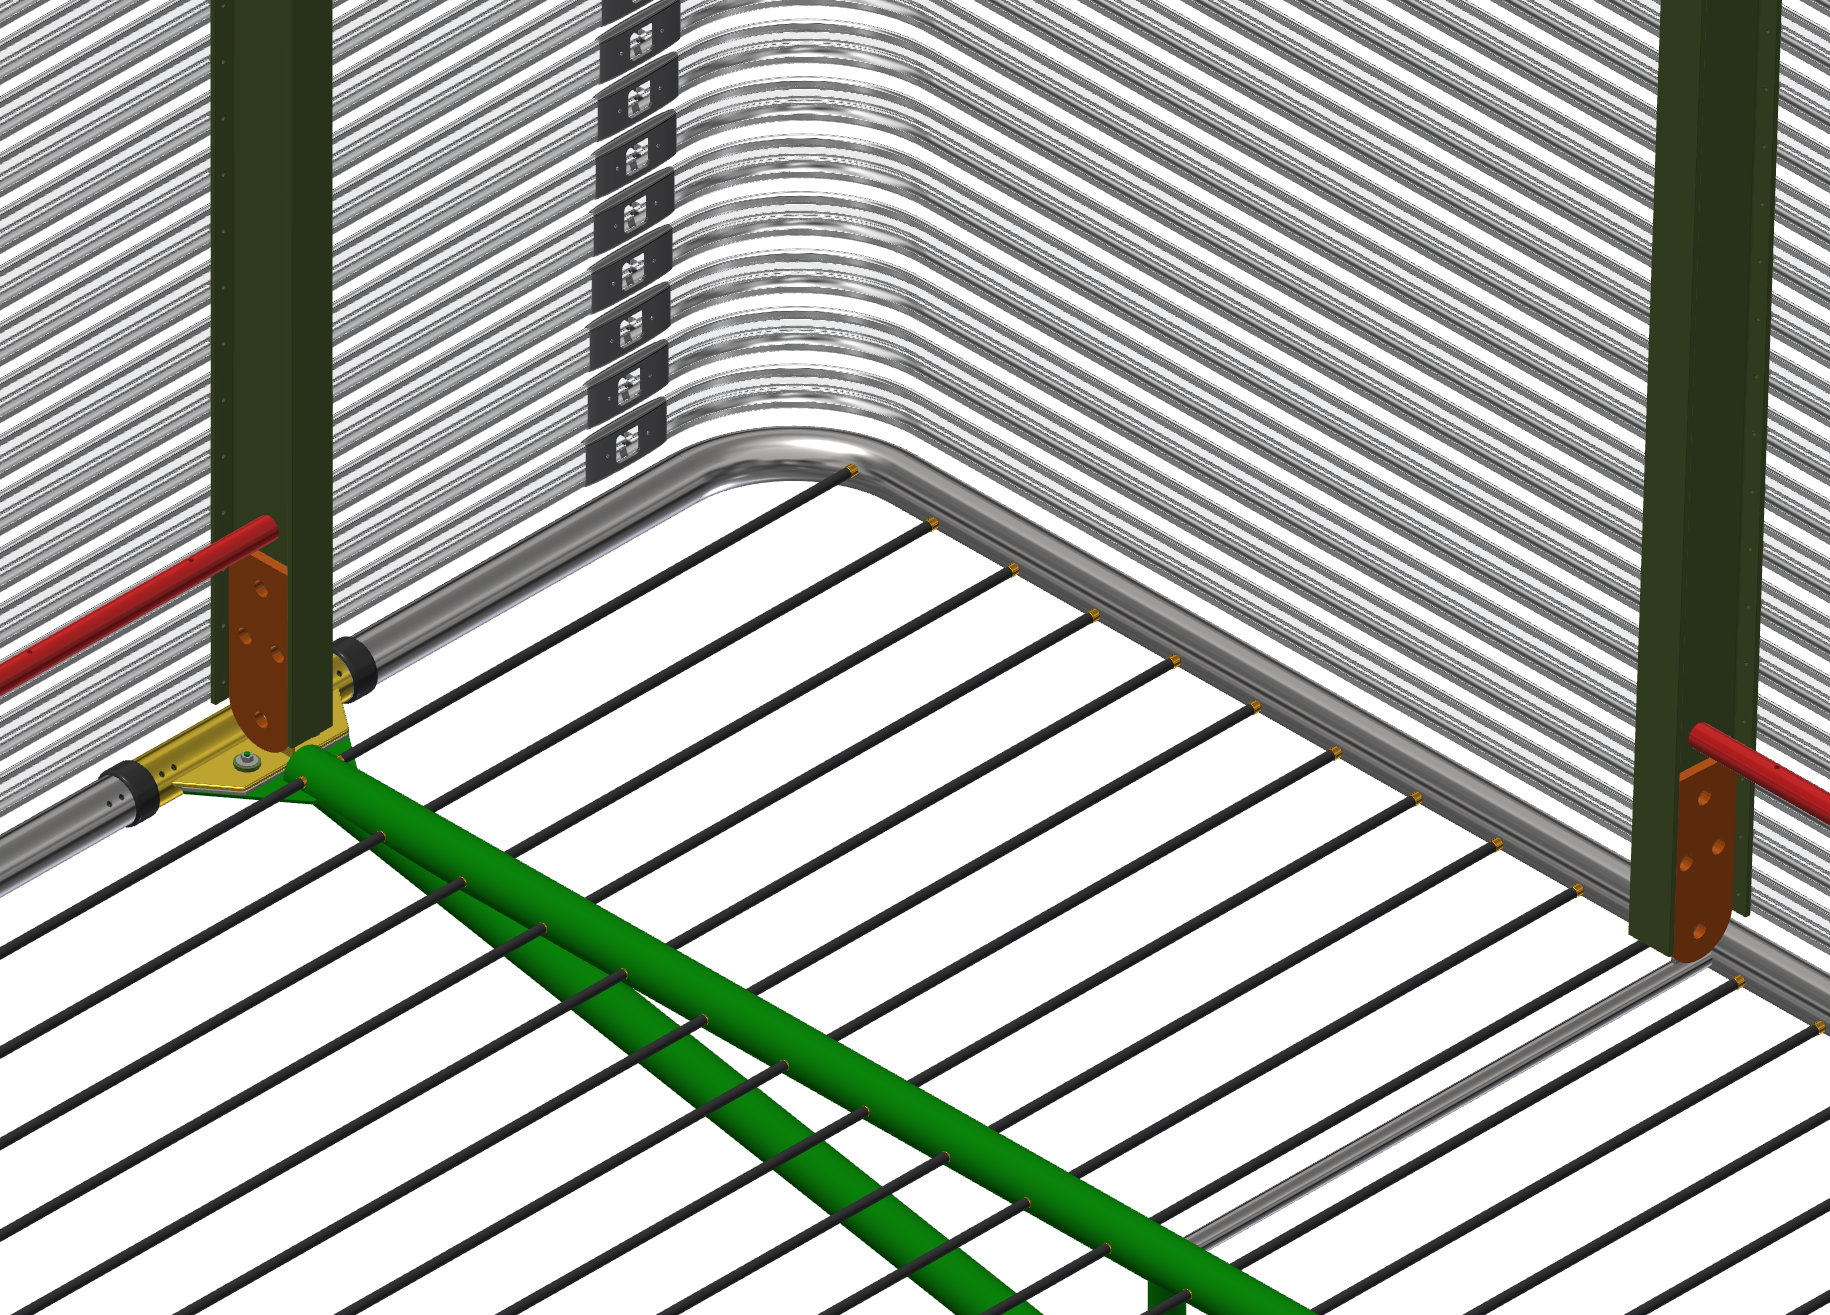
\includegraphics[width=0.9\textwidth]{DP_HVS_EW_corner_details.png}
\end{dunefigure}


The \endwall \dword{fc} modules %also 
have a slightly larger pitch between the \dword{fc} profiles to ensure proper alignment when tilted at the designed angle and are therefore  %.  These profiles are also 
mounted with a slight angle against the \dword{frp} I-beams by means of tapered spacers. % to compensate for the tilt angle.


Approximately \SI{500}{\N} of force is needed to keep the \endwall \dword{fc} super-modules inclined. This force is transferred through the interconnected cathode outer tubes to keep the %opposite \endwall super-module inclined in a symmetrical pattern. 
two \endwall{}s symmetrical. There will be a few centimeters of sag in the middle of the \endwall{}s that will not affect  \dword{tpc} operation.   

%The \dword{fc} is modular, each module covering a vertical area of \SI{4}{\m} (W) $\times$ \tpcheight (H). 
%There are two types of modules, straight section and corner, both types having the dimensions \SI{4}{\m} (W) $\times$ \tpcheight (H). A total of \num{76} straight section modules (i.e., with straight profiles) and four corner section modules, with profiles bent \num{90} degrees at one corner to allow straight connections via resistive sheaths around the corner on the straight section on the SWSM, as shown in Figure~\ref{fig:dune-dp-fc-all}.c.  A photo of the \dword{pddp} \dword{fc} is shown in Figure~\ref{fig:dune-dp-fc-all}.d.

Each \SI{12}{\m} module has one top submodule with \num{33} profiles, four middle submodules with \num{33} profiles each, and one bottom submodule with \num{34} profiles, a total of \num{199} profiles per module. 
The nominal voltage of the top-most field-shaping ring is \SI{-9}{\kV}. 
The top submodule makes the mechanical connection to the ceiling of the cryostat from which the entire \dword{fc} hangs (see Figure~\ref{fig:dp-fc-installation-connection}, left). The bottom modules make both mechanical and electrical connections to the cathode. % as depicted in Figure~\ref{fig:dp-fc-installation-connection} right.
Figure \ref{fig:dune-dp-fc-interconnection} shows the interconnection details between the \dword{fc} submodules (left) and between the bottom \dword{fc} submodule and the cathode structure (right).

\begin{dunefigure}[FC  interconnections]{fig:dune-dp-fc-interconnection}
{Left: Interconnect details between \dword{fc} submodules; Right: Interconnect details between the bottom \dword{fc} submodule and the cathode structure. All metal fasteners used here align with the centers of nearby \dword{fc} profiles and connect electrically to the \dword{fc} profiles at the same height (Credit: BNL). }
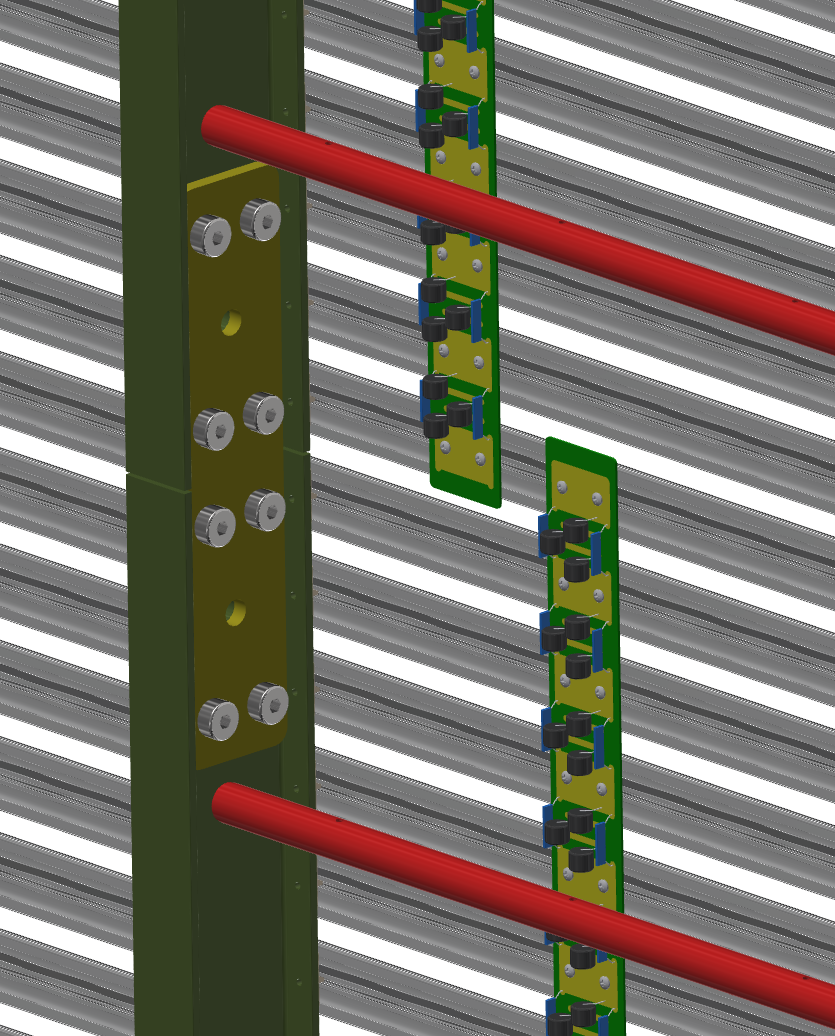
\includegraphics[width=.45\textwidth]{DP_HVS_FC_module_interconnect_details.png}
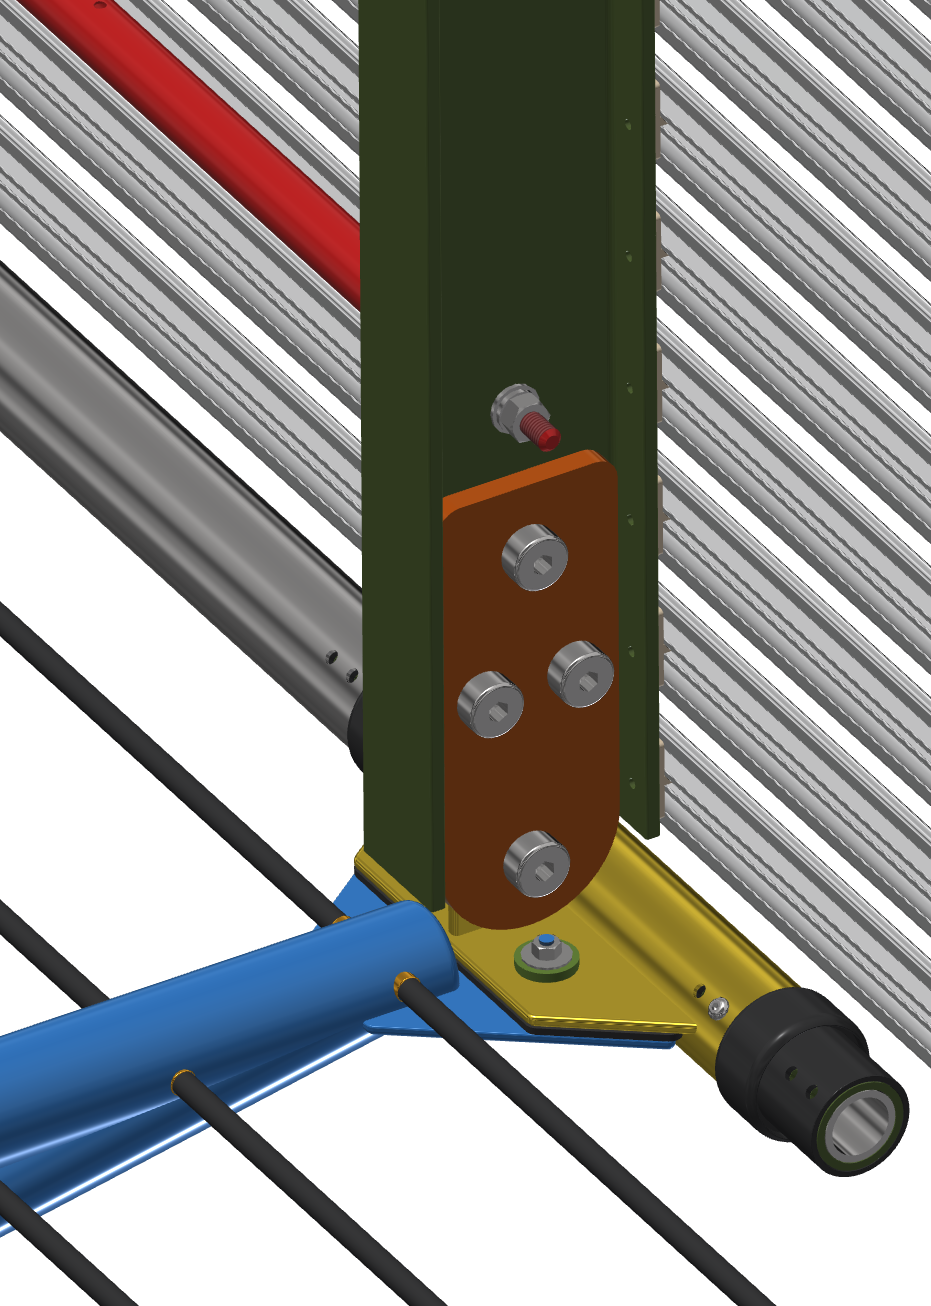
\includegraphics[width=.4\textwidth]{DP_HVS_FC_cathode_connection_details.png}
\end{dunefigure}

\subsection{Electrical Interconnections}

%A railed rib runs along the length of the aluminum profiles at the center of the profile.  The rib provides mechanical strength and acts as the rail for the slip nuts that hold the profiles onto the supporting \dword{frp} frame. The rib also serves as a rail for the square nuts that hold the \dword{hv} divider boards for both mechanical and electrical connections, and the nuts for securing the resistive sheath whose CAD drawing is shown in Figure~\ref{fig:resistive-sheath} a. 
A rib runs down the center of each aluminum profile to provide mechanical strength and act as a rail for the slip nuts that hold the profile onto the supporting \dword{frp} frame. The rib also serves as a rail for the square nuts that hold the \dword{hv} divider boards for both mechanical and electrical connections and the nuts for securing the resistive sheath (see  Figure~\ref{fig:resistive-sheath} a). 
%All profiles at a given height are electrically connected via a resistive sheath screwed onto the nut in the center railed rib across each set of two neighboring profiles as shown in the photos in Figure~\ref{fig:resistive-sheath} b and c with a 3D printed mock up plastic sheath with a profile inserted and screwed onto the sheath with a metal screw for a secure electrical connection. 
The set of all profiles at a given height are electrically connected together, end to end. Each neighboring pair is connected via a resistive sheath screwed onto the nuts in the center ribs across the two profiles, as shown in Figure~\ref{fig:resistive-sheath} b and c. These images show a \threed{}-printed mock up plastic sheath with a profile inserted and connected to it using metal screws to allow  electrical conduction. 

\begin{dunefigure}[\dual FC resistive sheath]{fig:resistive-sheath}
{a: A CAD drawing for the resistive sheath with a smoothed edge b: A cross-sectional photograph of the mock up plastic sheath screwed onto the profile center rib; c: The bottom view, active volume side, of a sheath connecting two neighboring profiles.} 
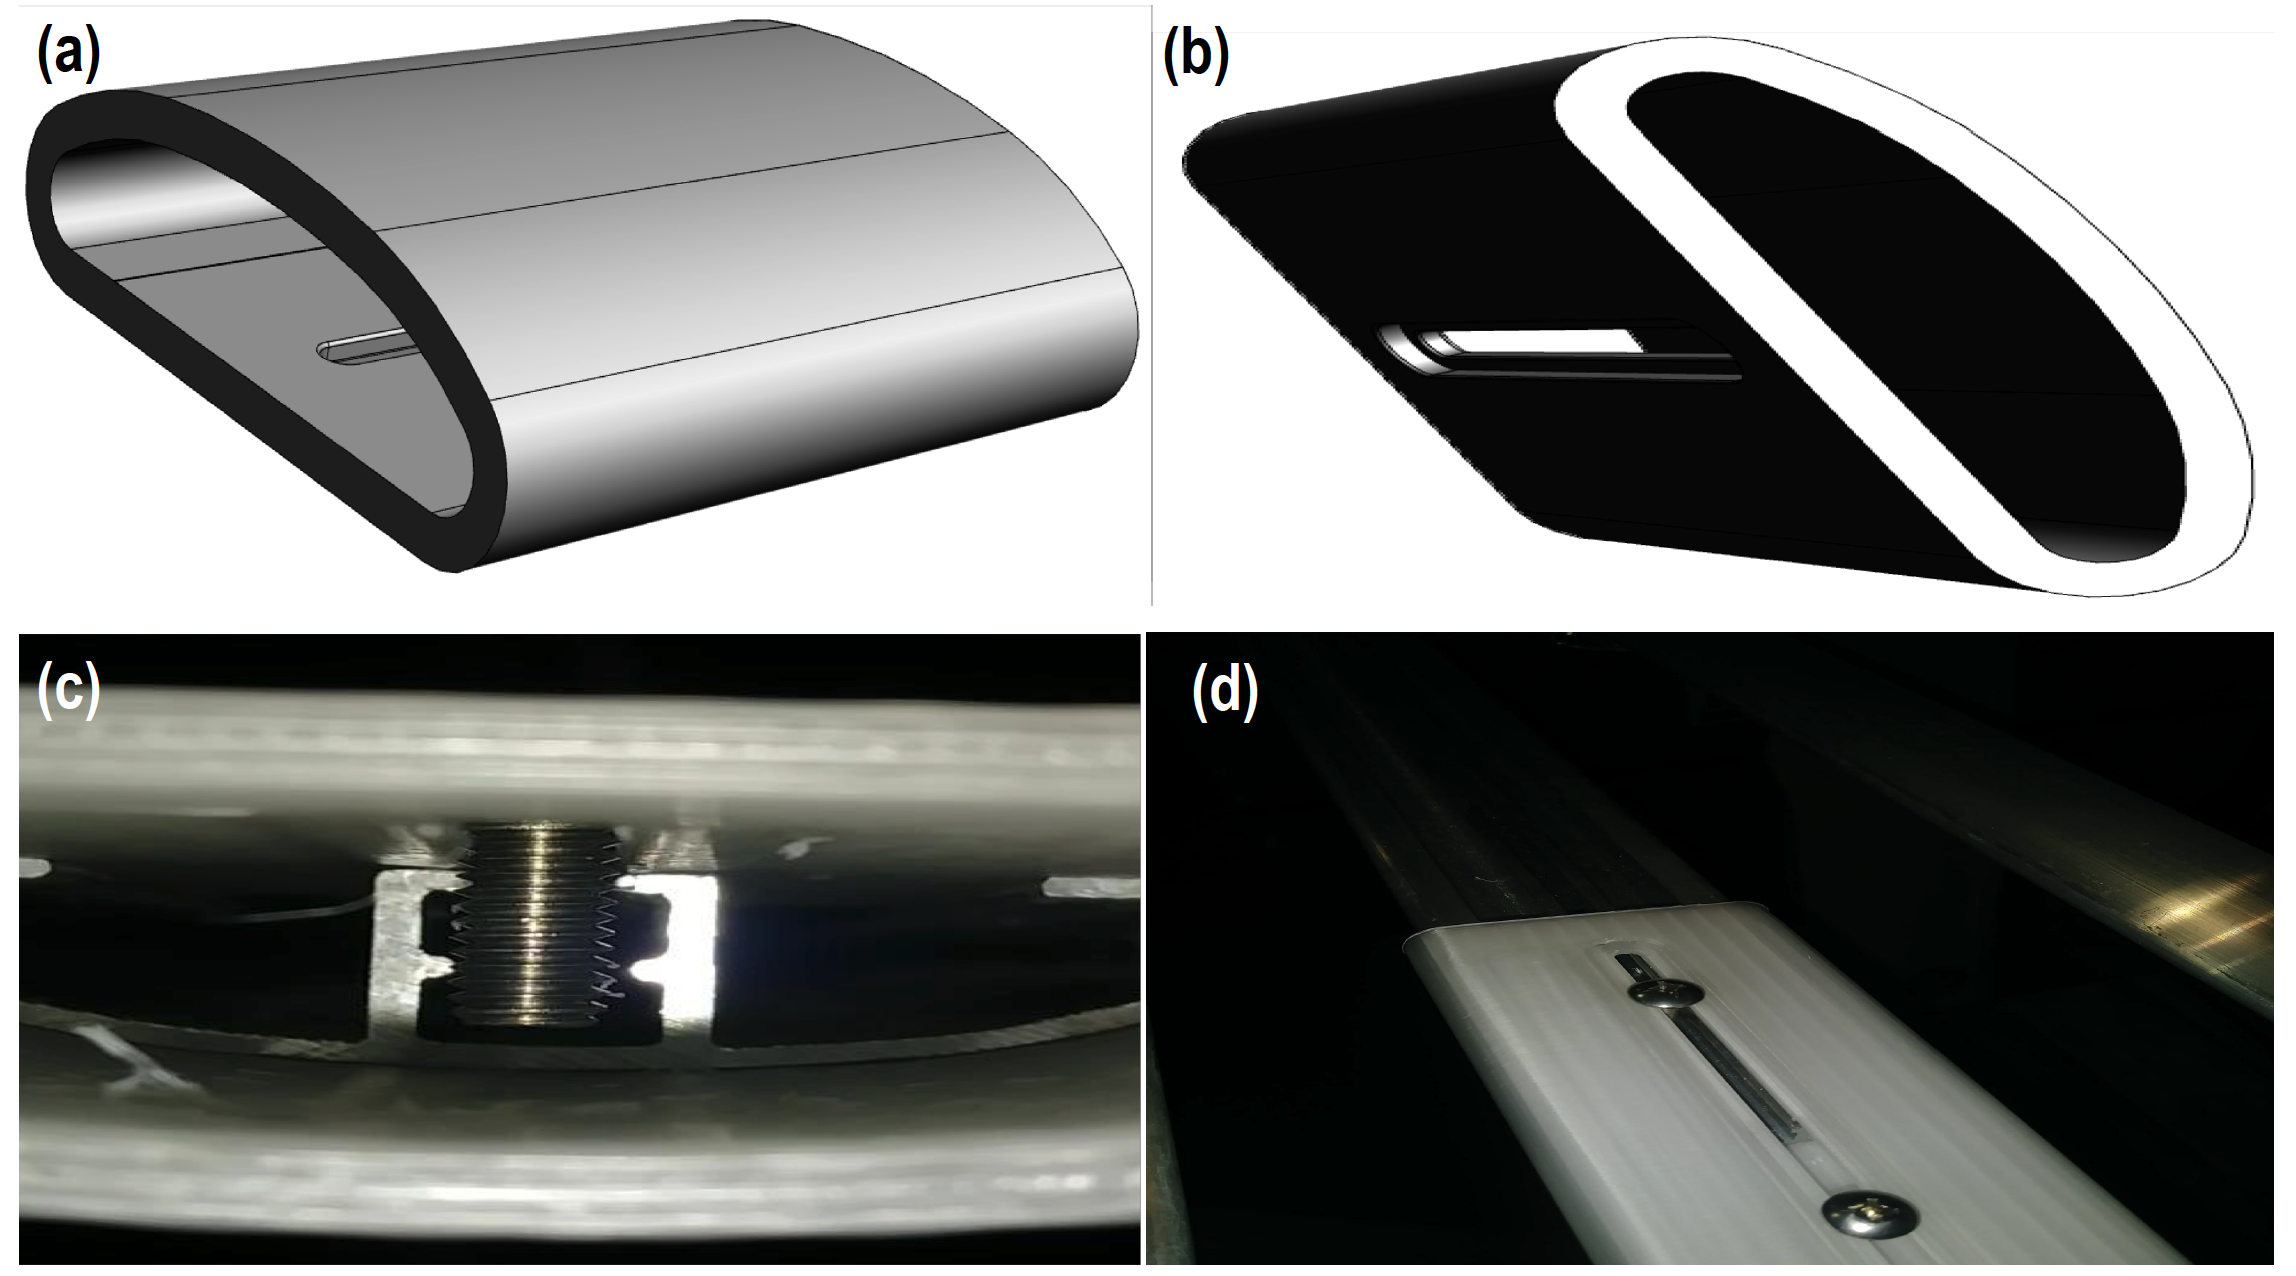
\includegraphics[width=0.8\textwidth]{DP_HVS_FC_Profile_Resistive_Sheath.png}
\end{dunefigure}

The resistive chain for voltage division between the profiles provides a linear voltage gradient between the cathode and the top-most field-shaping ring. This chain is critical because it determines the strength of the \efield between one profile and its neighbors as well as between the profile and other surrounding parts like the grounded stainless steel cryostat membrane. 
The \efield must be kept well below \SI{30}{\kV\per\cm} at all points in the \dword{lar} bath to keep \dword{tpc} operation safe (see Table~\ref{tab:hvphysicsreqs}). % the requirement table.

Each stage of the \dword{hvdb} consists of two \SI{5}{\giga\ohm} resistors in parallel for inter-board redundancy and two variable resistors of threshold voltage \SI{2}{kV} to protect the resistors in case of a sudden discharge.  With \num{199} stages under \dptargetdriftvoltneg  potential, the total expected current at \dptargetdriftvoltneg is, therefore, \SI{1.2}{\micro\ampere} per row of \dword{hvdb}.  
A total of \num{12} rows, one per super-module, connected in parallel, will be used for ample redundancy in the \dword{dune} \dword{dpmod}, yielding an expected overall current in the %entire 
\dword{fc} system of \SI{14.3}{\micro\ampere}.
For optimization, one \dword{hvdb} will connect \num{11} stages.  %This means  one \tpcheight tall module can be covered by eighteen \num{11} stage \dword{hvdb} and one \num{1} stage \dword{hvdb} at the bottom to make the final connection between the bottom most field-shaping ring and the cathode.
Thus eighteen \num{11}-stage \dwords{hvdb} are required for one \tpcheight tall module,  and one \num{1}-stage \dword{hvdb} is required at the bottom to make the final connection between the bottom-most field-shaping ring and the cathode.


Figure~\ref{fig:pddp-hvdb} shows one \dword{pddp} \dword{hvdb} board and  Figure~\ref{fig:dune-dp-fc-all}(d) shows the connection of one row of \dwords{hvdb} strung vertically along the entire height of the \dword{fc} as installed in \dword{pddp}. %The \dptpcwdth (W) $\times$ \dptpclen (L) ground plane consists of \num{80} unit planes (each \SI{3}{\m} $\times$ \SI{3}{\m}).  
The cathode plane is mounted on the bottom of the \dword{fc}, together forming one contiguous unit of field-providing structure.  The bottom-most %one stage 
\dword{hvdb} makes the connection between the cathode and the bottom-most field-shaping ring.
%As discussed above, \dpmod will install one \dword{hvdb} row for each super-module, employing a total of 12 rows, providing additional redundancy.  


\subsection{HV Return and Monitoring Devices}

To maintain the potential difference between the top-most field-shaping ring and the extraction grid of the \dword{crp}, either a dedicated \dword{hv} supply or an adjustable resistor chain is used in the \dword{hv} return outside the cryostat. %\fixme{The previous sentence needs some clarification. "Either" requires an "or", but in this sentence, we have either/and. Do you need both the HV supply and the resistor chain? Or is it one or the other, but not both?}  
This requires an independent \SI{10}{kV} \fdth similar to those developed for the extraction grid.
The current \dword{pddp} configuration can test both schemes.
The decision on which to use will be based on the \dword{pddp} experience.

Several devices will monitor the \dword{hv}:  
\begin{itemize}
\item The Heinzinger units have typical sensitivities down to tens of nanoamperes with current readback capability.  The units can sample the current and voltage every few \SI{100}{\milli\s}.  
\item Inside the cryostat, so-called pick-off points near the anode will monitor the current through the \dword{hvdb} resistor chain. Additional pick-off points could be implemented on the \dword{gg} below the cathode to monitor possible stray currents.
\end{itemize}


\section{Quality Assurance and Quality Control}
\label{sec:fddp-hv-qa}

\subsection{Field Cage}

%When \dword{frp} I-beams and other parts are delivered, they all undergo a visual inspection to look for defects, in particular those affecting structural integrity, such as cracks, air bubble holes, depression, and flatness. The parts are sorted into three preliminary categories: category 0 (pass), category 1 (problematic but repairable), and category 2 (severe and unusable).
When received, \dword{frp} I-beams and other parts are visually inspected for defects, in particular those affecting structural integrity, such as cracks, air bubble holes, depressions, and variations from flatness. The parts are sorted into three preliminary categories: category 0 (pass), category 1 (problematic but repairable), and category 2 (severe and unusable).

The visual inspection is followed by critical dimension measurements to verify individual submodule assembly and module interconnection integrity.  These measurements focus on cross sectional dimensions for rods, plates, and bars, as well as length, straightness, flatness, and camber of the beams and flanges.
All measurements must satisfy the mechanical tolerances in the design drawings and standard industry quality criteria.

The \dword{frp} I-beams and parts in category 1 are repaired during the preparation stage. %through defibering, deburring, and sanding
 Another set of measurements after the repair determines any changes in the part's category.

Those in category 2 are returned to the vendor for replacement.

All \dword{frp} parts that pass inspection are prepared for use, which involves \dword{qc} at each step.  Each part is first defibered, deburred, sanded to smooth the edges, then varnished to
suppress any remaining fibers. %\fixme{wait, this was only done on category 1. Sounds like it's done or redone on all. Anne} 
Once the part is prepared, it is stored in a humidity- and temperature-controlled drying area for \numrange{24}{48} hours to fully cure the varnish.  After full curing, each module is laser-engraved with a unique part number and recorded in a \dword{qc}  database. %\fixme{coordinate with IIC chapter for DP volume. Anne}

At this point, before the submodule is packaged, it is pre-assembled on a table to ensure all parts fit, including inserts, screws, and slip nuts. When fitness is verified, the submodule is disassembled, and all components are packed along with  \numrange{10}{20}\% spare hardware parts to ensure that each package is self-sufficient for final assembly. The submodule and all parts are shrink-wrapped into a compact package \SI{10}{\cm} $\times$ \SI{10}{\cm} $\times$ \SI{2}{\m},  and the edges are wrapped with thick plastic sheets to protect the parts from %mechanical damage from falls or other accidents. 
potential mechanical damage. %This package will contain all necessary parts to assemble the given sub-module and \numrange{10}{20}\% spare hardware.  This ensures that each package is self-sufficient for final assembly.  
Each package is given a submodule number for further tracking.  This submodule number stays with it throughout assembly at \dword{surf} and final installation, so the submodule can be assigned to a specific module, checked, and recorded once it is installed in the module. 

%%%%%%%%%%%%%%%%%%%%%%%%%%%%
\subsection{Electrical Interconnections and HV Divider}
\label{sec:fddp-hv-prod-interconnect}

{\bf Resistors, Varistors, and \dwords{hvdb}:} All resistors used for \dword{hvdb} production are numbered and undergo a three-stage %\dword{qa} 
\dword{qc} test for final selection. Resistance is measured at voltages up to \SI{4}{kV} in \SI{500}{V} steps for each stage. The first stage of testing is done at room temperature, the second in \lntwo, and the third again at room temperature after warming the resistors up again.  For final selection, the measured values are placed in a histogram  to locate groupings of resistance values. The resistance values should be closer to each other than at any particular value (unless they deviate too far from the design values). The resistors for which the resistance values are within 1\%  of each other are selected.%   \fixme{I reworded the prev paragraph}

All varistors for board production are also numbered for \dword{qa} purposes and undergo a three-stage \dword{qa} 
%\fixme{are we sure this is QA not QC?}
testing program for final selection. Each test stage is a clamping voltage measurement, first at room temperature, then at \lntwo temperature, and again after warming the varistors back up to room temperature. The measured values are placed in a histogram for final selection; to ensure proper protection, those with clamping voltages closest to the design values are selected.

Once the parts are selected, they are sent to the vendor for mounting.  When the completed \dwords{hvdb} are delivered, they undergo a three-stage \dword{qa} testing program. Each stage involves a resistance measurement of the whole board, and at each stage, the board is teasted first at room temperature, then in \lntwo, and again after warming the boards back up to room temperature.  The measured resistance values are placed in a histogram for final board selection. 
The boards can fall into one of three categories: category 0 (pass), category 1 (problematic but repairable), and category 2 (severe and unusable). 
%0 Pass, 1 Repairable, and 2 Rejected. 
%\fixme{can we make this the same as above? 0 (pass), category 1 (problematic but repairable), and category 2 (severe and unusable).}
If at any testing stage the resistance is more than \SI{0.5}{\%} away from the mean, the part does not fall into category 0. %Boards in category 1 are sent back to the vendor with the selected resistors, so the parts in failed stages can be replaced with the resistors selected during the QA. 
Boards in category 1 are sent back to the vendor with the selected resistors, so that the parts that failed one stage or another can be replaced with resistors selected during the \dword{qa}. %\fixme{QC?}

{\bf Aluminum Profiles and Resistive Sheath:}
The \dword{qa} testing of the aluminum profiles and the resistive sheath uses prototype production samples before full production begins.   The samples are visually inspected for shape, adherence to the design drawing, and surface smoothness, surface-coating quality, and smoothness of the bend (for profiles with the \num{90}$^{\circ}$ bend).  

The resistive sheath samples are visually inspected for shape, adherence to the design drawing, edge smoothness, resistance, and mechanical fitness, as well as for how tightly they fit to the profiles while still allowing %an easy slide to couple 
easy coupling to the neighboring profile and good electrical contact.
Each sheath is numbered and undergoes %an identical 
a three-stage \dword{qa} test, %as for 
similar to the resistors, for final selection. Resistance is measured at voltages up to \SI{4}{kV} in \SI{500}{V} steps for each stage: at room, \lntwo{}, and again room temperature. %The first stage of testing is done at room temperature, the second in LN2, and the third again at room temperature after warming up.  
For final selection, the measured values are placed in a histogram to look for groupings of resistance values.   


{\bf Power Supply and Feedthrough:} The power supply is tested extensively along with the controls and monitoring software.  %Features to be included in the software \fixme{tests?} are:
Tested capabilities include
\begin{itemize}
\item Ramping and changing the set voltage, including ramp-rate change and pause capabilities and settings; 
\item Acceptance of a user-defined current limit:  this parameter sets the %value of current at which the supply reduces the voltage output to stay below the set current limit.  
maximum value of current; at this point, the supply must reduce the voltage output;
\item Acceptance of a setting for the trip-threshold current:  %at this threshold, the software would reduce the voltage output. 
at this point, the supply must reduce the voltage output.  
(In previous experiments, the trip function in software would set the output to \SI{0}{kV}.); and
\item Recording the current and voltage readback values with a user-defined frequency and recording of any irregular current or voltage events. 
\end{itemize}


%\subsection{Quality Control}
\subsection{Quality Control During Assembly and Installation}
\label{sec:fddp-hv-transport-qc}

%\fixme{need to resection a bit, not a parallel structure. Anne will think about it. This section should probably be in the IIC chapter}
Assembly, testing, transportation, and installation procedures must ensure adequate \dword{qc} of all \dword{hv} system components. The entire assembly and installation of the \dword{hv} system will be performed at \dword{surf}.% are being defined, tested and documented during the construction of \dword{pddp}.

%\fixme{starting from here, it sounds like everything is done at SURF, no? anne}
The \dword{fc} submodules are assembled inside the cryostat on an assembly table with a precision alignment bar. %, as in \dword{pddp}.  %A sub-module FRP part package will be visually inspected for any external damages and will be opened carefully to avoid any damage to the FRP parts.  
Each submodule package is visually inspected for external damage and is opened carefully to avoid damage to the \dword{frp} parts.  
Bags of hardware are removed and set aside. 
The two \SI{10.2}{\cm} (\SI{4}\,in) \dword{frp} I-beams, two stainless steel cross bar tubes with diameters of \SI{2.5}{cm} (\SI{1}{in}), and connecting brackets are visually inspected for any damage incurred during transport. Once these parts pass inspection, they are assembled onto the frame on the assembly table.  
The aluminum profiles are visually inspected and felt by hand for severe scratches and sharp points.  The profiles that pass are placed onto a flange of the \dword{frp} I-beams, with %one slip nut each 
a slip nut inserted into the rail on the profile reinforcement rib on either end. 
Assembly and alignment follow the process described in Section~\ref{sec:dp-hv-assembly}. The alignment of the profiles is checked using a straight-edge along one end of the profiles.  The submodules that pass are put on the wheel base and stored until they can be installed. %\fixme{what's the wheel base?}

The \dword{hv} divider boards are visually inspected for any damage incurred during the transport, and the resistance of each stage is tested on-site at room temperature to ensure the integrity of the board and the electrical connections of the resistors before installing the boards onto the submodule. 
%\fixme{Unless the previous stuff was NOT at surf, let's not say 'at surf' now. Below it talks about a 'test setup'. Please clarify where things are done and in what order. I'm a little confused! (anne)}
%At \surf, 
Cathode and \dword{gg} modules are checked for the required planarity and mechanical integrity. 
%\fixme{what phase is the previous done in? anne}
In addition, during the installation phase, the electrical continuity between the modules is checked.

The \fdth and the \dword{hv} extender are tested simultaneously  at \dword{cern}, %\fixme{need new plan - no more ITF. tested underground with the actual power supply?} 
preferably with the power supply to be used in the detector. 
To pass, the \fdth must hold the target voltage (\dptargetdriftvoltneg{}) in ultra-pure \dword{lar} (\dword{tpc}-quality purity corresponding to a free electron lifetime, $\tau\geq$\SI{7}{\ms}) for at least \num{24} hours. The ground tube submersion and \efield environment of the test set up must be comparable to the real \dword{fc} set up or a more challenging environment. Additionally, the \fdth must be UHV-grade leak tight.

Upon arrival at \dword{surf}, the power supply used in the \dword{dune} \dword{dpmod} \dword{hv} system is tested before installation, with output voltages and currents checked on a known load. 

\noindent 
%%%%%%%%%%%%%%%%%%%%%%%%%%%%
\section{Safety}
In all phases of \dword{hv} system deployment of the \dune \dpmod, including fabrication, installation, and operations, safety is the highest priority.  As was done for \dword{pddp}, all assembly, testing, transport, and installation procedures will be documented. Explicit attention is paid to how well \dword{pddp} procedures transfer to the \dpmod. The most critical of these are noted in the preliminary \dword{hv} risk assessment (see Section \ref{sec:fddp-hv-org-risk}). %\fixme{add reference}
%\fixme{This section will discuss interaction of HV experts withIntegration team, and reference the appropriate chapter/volume for further details.}

\subsection{Production Safety}
\label{sec:fddp-hv-prod-safety}

%The \SI{10.2}{\cm} (\SI{4}\,in) \SI{2.0}{\m} long \dword{frp} I-beams are delivered with screw holes already drilled to hold aluminum profiles. These I-beams must be processed to eliminate any remaining fiber or slivers of plastic. This requires a set process already tested at \dword{pddp} \dword{fc} module production. Sanding, deburring, and varnishing prepare I-beams, and preassembly verifies the fitness of the parts. The \SI{2.54}{\cm} (\SI{1}\,in) \SI{2.0}{\m} long stainless steel cross bars must be filed and sanded to remove chips and slivers.
%The \SI{10.2}{\cm} (\SI{4}\,in) \SI{2.0}{\m} long \dword{frp} I-beams 
%\fixme{make sure numbers match table 1.2} are delivered \fixme{to the production site? Where is that?} with screw holes already drilled to hold aluminum profiles. 
%\fixme{who performs this sanding, etc. process? "Personnel participating in the production process"?} A set process of sanding, deburring, and varnishing, already tested during \dword{pddp} \dword{fc} module production, will be followed to eliminate any remaining fiber or slivers of plastic.  This process and preassembly together verify the fitness of the parts. The \SI{2.54}{\cm} (\SI{1}\,in) \fixme{thick?}  \SI{2.0}{\m} long stainless steel cross bars must also be filed and sanded to remove chips and slivers.

Personnel participating in production will be thoroughly trained %be trained thoroughly for 
on the hazards in the process.  
Pallet jacks, dollies, and hoists will be used for lifting to avoid injuries from moving heavy equipment. 
Personnel will be trained to avoid back injury using the site's prevention procedures and avoid overextending as they lift and move parts and equipment.  % as a preventive measure.
%Personnel 
I-beam and the stainless steel tube manipulation will require %be done with 
extreme care to avoid injury %to any personnel or 
as well as damage to any parts or equipment. 
Personnel will take care %will be taken 
to avoid spilling liquid (ethanol, Simple Green\texttrademark{} cleaner, varnish, or de-ionized water) on the floor to prevent slips and falls %slippage, 
and will mop up  any spilled liquid %will be mopped 
immediately. 
%with a floor mop.
%\fixme{Is Simple Green the only option for cleaner? If not, should this be more generic? anne}
All personnel will use gloves, protective glasses, and masks while working with ethanol, epoxy, varnish, and cleaner. %Simple Green. 
They %Users will have 
will use the appropriate respiratory protections following the production site's respirator program rules and receive respirator training as
required.

\subsection{Handling Safety}
\label{sec:fddp-hv-transport-safety}
%\subsection{Assembly and Installation}
%\label{sec:fddp-hv-install}

The structural and electrical designs for the \dword{dune} \dword{dp} \dword{hv} system are based on designs vetted and validated in \dword{pddp} construction, which %is currently 
 is in its final phase of deployment at \dword{cern} as of April 2019. In parallel with the \dword{pddp} construction and operation, \dword{hv} tests at \dword{cern} were performed using full-voltage and a full-scale \dword{hv} \fdth, power supply, and monitoring system in dedicated \dword{hv} test facilities. This has also provided an opportunity to complete full safety reviews. 
Operating the \dword{fc} at its full %operating 
voltage produces a substantial amount of stored energy. The modular design of the cathode specifically addresses this safety concern: in the event of a power supply trip or other failure that unexpectedly drops the \dword{hv}, %the charge stored in the segmented cathode structure limits the power dissipated. 
the segmented cathode structure prevents the stored charge from crossing to neighboring cathode modules, thus limiting the power dissipated. %\fixme{please check my rewrite above. anne}
%This design will be tested in \dword{pddp} at \SI{-300}{kV} voltage over \SI{9}{\m$^2$} surface segmented in each of the four cathode modules.  
%This feature of the design will be tested in \dword{pddp} at \SI{-300}{kV} over a \SI{9}{\m$^2$} cathode surface segmented into four cathode modules. 

Integral to the \dword{dp} \dword{fc} design, both in \dword{pddp} and the \dword{dune} \dword{dpmod}, %is the concept of 
are the pre-assembled modular panels (called \dword{fc} submodules) of field-shaping %conductors 
profiles with individual \dwords{hvdb}. %voltage divider boards. 
The structural design and installation procedures used in \dword{pddp} were %selected 
developed as prototypes for use  %to be compatible with use 
at the \dword{fd} site and were vetted by project engineers, engineering design review teams, and \dword{cern}'s safety engineers. Some revisions to these designs are expected based on lessons learned in \dword{pddp} installation and operations. These revisions will be reviewed both within the \dword{dune} project and by \dword{fnal} \dword{esh} personnel. The up-front attention to %safety 
potential hazards, personnel preparation, and use of equipment puts the  overall \dword{dune} \dword{dpmod} \dword{hv} design 
on solid footing in terms of safety. %\fixme{check my edits above. anne}

Assembly of the \dword{fc} submodules and %resistor-divider boards 
\dwords{hvdb} involves labor from the collaboration members, technical staff, and students and  does not present unusual industrial hazards. The \dword{hv} consortium will work closely with each production site 
%\fixme{different from production site?} 
to ensure that procedures meet both \fnal{}'s and institutional requirements for safe procedures, personal protective equipment, environmental protection, %trained 
materials handling, and training. Most %production 
part fabrication will be done commercially, and shipping will be contracted through approved commercial shipping companies. Before a site is approved as a production venue, an external safety panel will visit the site for review to ensure best practices are in place and followed. 

\subsection{Operation Safety}
\label{sec:fddp-hv-operation-safety}
Given the proposed design of the \dword{hvs}, which does not expose any part of the system to a direct human contact, we do not foresee any additional safety issues for personnel.
We do, however, have interlocks on the \dwords{hvps} for the safety of the equipment if
\begin{itemize}
\item {\dword{lar} levels drop within 5 cm of the top of the rim of the ground of the HVFT}; \fixme{What is HVFT? The abbreviation is not in the common glossary.}
\item {Pressure relief valves are opened};
\item{Any other conditions occur that could cause \dword{lar} to boil at shallow depths};
\item {Overall detector resistance shows any sudden variation}.
\end{itemize}
%%%%%%%%%%%%%%%%%%%%%%%%%%%%%%%%%%%%%%%%%%%%%%%%%%%%%%%%%%%%%%%%%%%%
\section{Transport, Assembly, and Installation and Integration}
\label{sec:fddp-hv-transport}

%%%%%%%%%%%%%%%%%%%%%%%%%%%%
\subsection{Transport and Handling }
\label{sec:fddp-hv-transport-transport}

The \dword{fc} \dword{frp} I-beams, the stainless steel cross bar tubes, and other parts are shipped in standard wooden crates.  Parts for each submodule are packed into one compact flat pack \SI{0.1}{\m} $\times$ \SI{0.1}{\m} $\times$ \SI{2}{\m} and sealed in several layers of shrink wrap and a thick, soft cushion of plastic layers for edge protection. 
%\fixme{earlier it says .2 by .2 by 2. Pls reconcile - and maybe we can just say it once? Anne}
Because each submodule package is so compact, each wooden crate \SI{1.5}{\m} (H) $\times$ \SI{1.3}{\m} (W) $\times$ \SI{2.5}{\m} (D) can transport \num{110} submodule flat packs stacked \num{10} (W) $\times$ \num{11} (H).
The total number of submodule flat packs needed for the entire \dword{fc} is \num{216}, excluding spares, so all \dword{fc} frame parts can be transported in two crates. 
Each of these fully loaded crates %would 
will weigh less than \SI{2500}{\kg}.
The cage for underground transport at \dword{surf} is 
\SI{3.6}{\m} (H) $\times$ \SI{1.38}{\m} (W) $\times$ \SI{3.7}{\m} (D) with a load capacity of \SI{13000}{lbs}, or approximately \SI{6000}{\kg}, so, in principle, all \dword{fc} frame parts can be transported underground %in \surf 
in one cage trip. %\fixme{reconcile this with logistics - bringing them down together may be irrelevant depending on the cage scheduling. anne}

The extruded aluminum profiles for \dword{fc} are shipped separately in  standard wooden crates. In all, \num{199} profiles  $\sim$\SI{4}{\m} long are needed for each \tpcheight \dword{fc} module, for a total of %. Therefore, 
\num{7164} to transport %profiles must be transported 
underground, excluding spares. The same number of resistive sheaths are %also 
shipped separately in standard wooden crates. % and transported underground. 

The \SI{12}{\m} (L) $\times$ \SI{30}{\cm} (H) $\times$ \SI{2.5}{\cm} (W) trusses for the cathode modules  are welded off-site and shipped to \dword{surf} in transport containers. 
The \SI{12}{\m} (L) $\times$ \SI{2.5}{\cm} (D) resistive rods are also constructed off-site and shipped in standard wooden boxes. %Given the installation procedure and 
The installation procedure takes into account the lack of storage space at the 4850L, so cathode modules are transported underground in an assigned order, corresponding to their installation sequence starting from  %the cathode plane is assembled as each cathode unit arrives at the cavern in its assigned order since the \dword{fc} super-modules are assembled in sequence beginning at the opposite end of the cryostat from the \dword{tco}.
the end of the cryostat opposite the \dword{tco}; the same goes for the \dword{fc} super-modules. %\fixme{check my edits above. anne} 

The power supply, \fdth{}s, and \dword{hv} extender are sent to \dword{surf} in standard shipping crates. Unwrapping requires clean areas and careful handling. Surfaces can be cleaned with alcohol and allowed to dry.

\subsection{Assembly}
\label{sec:dp-hv-assembly}

%An \dword{fc} sub-module is pre-assembled on a table before packaging to ensure fitness of all parts, including all screws and slip nuts.   When fitness is verified, the sub-module is disassembled and packaged in a \SI{10}{\cm} $\times$ \SI{10}{\cm} $\times$ \SI{2}{\m} compact package with the edges wrapped in a thick plastic layer to protect the parts from mechanical damage from a fall or some similar accident.  This package includes all necessary parts to assemble the given sub-module along with \numrange{10}{20}\% spare parts. This ensures that each package is self-sufficient for final assembly. Each package is given a sub-module number for further tracking. This number stays with the sub-module throughout assembly at \surf and final installation, so the sub-module can be assigned to its specific module and in its proper location within the module. 

%The compact packages of the \dune \dword{dpmod} \dword{fc} parts are shipped to \surf and transported underground for final sub-module assembly prior to the installation. The \SI{4}{\m} long aluminum profiles are produced and shipped to \surf separately for final assembly. The final \dword{qc} of the profiles is conducted during sub-module assembly.   Profiles with deep scratches and sharp protrusions that could cause excess charge concentration will be rejected. This process must be done underground at the time of sub-module assembly because of the delicate nature of the coated surface and the smoothness requirement. %\fixme{I took out: of the smoothness to meet the local maximum field requirement.}

\dword{fc} submodules are assembled inside the \dword{dune} \dword{dpmod} cryostat. An assembly table with a precision alignment bar for rapid profile alignment is used for this task.  The submodule package is opened on the table, and the mechanical frame is assembled %using 
from two \SI{10.2}{\cm} (\SI{4}{in}) \dword{frp} I-beams and two \SI{2.5}{\cm} (\SI{1}{in}) diameter stainless steel tubes.

Once the frame is assembled, the aluminum profiles are mounted on the flange of the \dword{frp} I-beams and secured using two slip nuts inserted on either end and are secured with two button-head, hex-drive metal screws, with one side secured tightly and the other loosely, but solidly to allow motion from thermal contraction.  
The submodules designated for the middle %module 
of a super-module must have a square nut inserted  between the two slip nuts for \dword{hvdb} mounting. Care must be taken to avoid scratching %ensure that 
the profiles %are not scratched 
during the mounting process.  

When all screws are hand-tightened as much as possible, the final torque is applied using a power screwdriver with a preset torque. %the \SI{12}{\V} power screwdriver\footnote{Dewalt\texttrademark{} Power Screw Driver} torque set at \num{1}. 
The final alignment of the profiles is then made by hand, tightening only one or two screws on the tightly secured side as needed. 
A wheel base made of unistrut bars is then mounted to the bottom of the submodule, and the entire unit is placed in a designated area to await installation. Each submodule is clearly labeled with its %the designated sub-module 
tracking number.

Cathode modules will be %assembled on their location 
installed along with their neighboring %as 
\dword{fc} super-modules %are installed 
as described in Section~\ref{sec:fddp-hv-transport-install}.

%%%%%%%%%%%%%%%%%%%%%%%%%%%%
\subsection{Installation and Integration}
\label{sec:fddp-hv-transport-install}
%\fixme{This section may need to go into the DP IIC chapter. Anne}
All \dword{fc} submodules are assembled inside the cryostat on an assembly table as described in Section \ref{sec:dp-hv-assembly}. Resistive sheaths for submodule interconnections and the square nuts to hold \dword{hvdb} are pre-inserted to each profile at this stage.
Once a submodule is fully assembled, a transport wheel base is mounted on it, so it can be easily relocated.
When three top submodules, three bottom submodules, and \num{12} middle modules are assembled, %we begin installing them 
they will be installed as a super-module starting at the far end of the cryostat. %, opposite to the temporary construction opening.

The installation sequence for a super-module is described below and depicted in Figure~\ref{fig:dp-super-module-installation-secuence}:

\begin{enumerate}
    \item Hang a \SI{12}{\m} stainless steel I-beam from two stainless steel cables through the \fdth{}s and raise it to approximately \SI{2.5}{\m} above the temporary floor.
    \item Place three top submodules under the stainless steel I-beam, and connect each to the I-beam using two sets of stainless steel L-brackets, stainless steel inserts, stainless steel screws, stainless steel lock washers, and stainless steel nuts.  
    \item Slide the two resistive sheaths (pre-inserted into the middle submodule) over and tighten them onto the two neighboring profiles to make the resistive connections between profiles in the row. 
    \item Mount \dwords{hvdb} to the center submodule in the row, using aluminum button-head screws and a square nut pre-inserted in the profile reinforcement rail. This process completes one row of the submodules for a super-module (see Figure~\ref{fig:dp-super-module-installation-secuence}a). 
    \item  %The three-unit \dword{pds} reflector/\dword{wls} panel assemblies of dimension \SI{199}{\cm} (W) $\times$ \SI{186}{\cm} (H) (shown in Figure~\ref{fig:dp-pds-reflector-panel-assembly}) for the three middle surfaces in the row, and two extended \dword{pds} reflector/\dword{wls} panel assemblies of dimension \SI{290}{\cm} (W) $\times$ \SI{186}{\cm} (H) (not shown) for the two ends of the row are mounted 
    Mount the \dword{pds} reflector/\dword{wls} panel assemblies on the \dword{frp} I-beams of the \dword{fc}, starting from one end of the row and progressing toward the other, covering the entire surface (see Figure~\ref{fig:dp-super-module-installation-secuence})a'. The extended \dword{pds} reflector/\dword{wls} panel assemblies at the \endwall{} corner \dword{fc} submodules will be \SI{290}{\cm} (W) $\times$ \SI{186}{\cm} (H), whereas the assemblies at the side wall corner \dword{fc} submodules will be \SI{260}{\cm} (W) $\times$ \SI{186}{\cm} (H).
    %For the corner FC modules, three \SI{199}{\cm} (W) $\times$ \SI{186}{\cm} (H) and two extended \dword{pds} reflector/\dword{wls} panel assemblies of dimension \SI{290}{\cm} (W) $\times$ \SI{186}{\cm} (H) for end wall corner \dword{fc} modules or a \SI{260}{\cm} (W) $\times$ \SI{186}{\cm} (W) for side wall corner \dword{fc} modules, with the extension covering the corner side.
    
    %\fixme{I can't figure this out. The figure 18 doesn't show a three-unit anything. The dimensions don't quite match up. Anne}
    
\begin{dunefigure}[PDS reflector/WLS panel assembly for mounting onto FC]
{fig:dp-pds-reflector-panel-assembly}
{The \dword{pds} reflector/\dword{wls} panel assembly mounted on the \dword{fc} \dword{frp} I-beams. (a) The coated surface of the panel assembly, which faces the active volume. The blue bars represent the I-beams onto which the %reflector/\dword{wls} 
panel assembly mounts. (b) The uncoated reverse G-10 surface of the  %reflector/\dword{wls} 
panel assembly. % which faces away from the active volume.  
The six vertical (darker green) bars provide mechanical support to the %\dword{pds} reflector/WLS 
panel assembly.}
%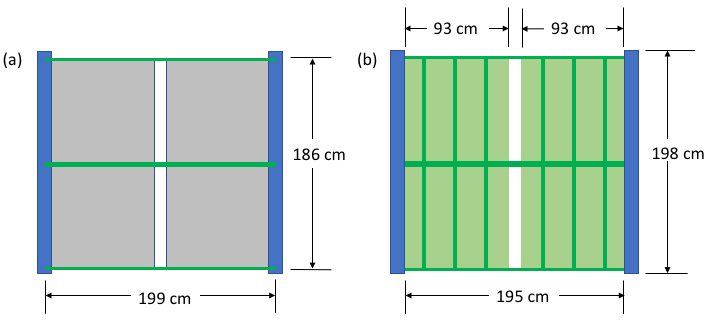
\includegraphics[width=0.9\textwidth]{graphics/DP_HVS_FC_PDS_Reflector.png}
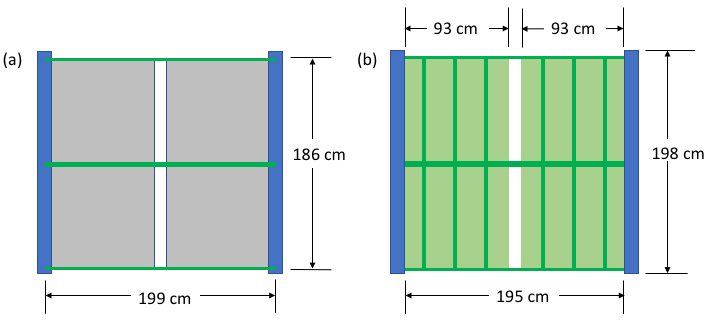
\includegraphics[width=0.9\textwidth]{graphics/DP_HVS_FC_PDS_Reflector.png}
\end{dunefigure}

     The extension of the assemblies to be mounted at corner ends of the side wall \dword{fc} modules is much shorter than the other extended modules %\fixme{than the extensions on the other modules?} 
     to safely accommodate the \num{2.4} degree tilt of the end walls. The panel assemblies are described in Section\ref{sec:dp-pds-mechanics} and the installation procedures in Section\ref{subsec:dp-pds-undergroundinstallation}.
    \item Raise the completed top row by approximately \SI{2.5}{\m}, place three middle submodules under the top row, and connect each %of the three middle sub-module 
    to %each 
    the corresponding top submodule above using \SI{1}{\cm} thick G-10 connection plates and stainless steel screws and nuts (see Figure~\ref{fig:dp-super-module-installation-secuence}b).
    \item %Once all middle modules are connected to the corresponding top sub-modules, s
    Slide the two resistive sheaths %pre-inserted into 
    in the center submodule over and tighten them onto the profiles to make the electrical connections between the submodules. %\fixme{I don't see this in 19b. Anne}
     
    \item Mount \dword{hvdb}s to the middle module using aluminum button-head screws and a square nut. 
   \item %The three unit \dword{pds} reflector/\dword{wls} panel assemblies of dimension \SI{199}{\cm} (W) $\times$ \SI{186}{\cm} (H) and two extended \dword{pds} reflector/\dword{wls} panel assemblies of dimension \SI{290}{\cm} (W) $\times$ \SI{186}{\cm} (H) are mounted on the \dword{frp} I-beams of the \dword{fc} at this stage 
   Mount the \dword{pds} reflector/\dword{wls} panel assemblies onto the \dword{frp} I-beams of the \dword{fc} 
   starting from one end of the row and progressing towards the other, covering the entire surface (see Figure~\ref{fig:dp-super-module-installation-secuence}b'). 
   
    \item Repeat steps \num{6} through \num{9} %above one more time 
    once to complete the assembly of the top half of the super-module %covered with the 
    and \dword{pds} reflector/\dword{wls} panel assemblies, (see Figure~\ref{fig:dp-super-module-installation-secuence}c and c').
    \item Repeat steps \num{6} through \num{8} %above 
    three more times to complete the assembly of the %remaining 
    bottom half of the super-module (see Figure~\ref{fig:dp-super-module-installation-secuence}d).
\end{enumerate}

\begin{dunefigure}[FC super-module installation sequence for \dpmod ]
{fig:dp-super-module-installation-secuence}
{\dword{fc} super-module installation sequence. The red bar at the top of each diagram is the stainless steel I-beam. The white vertical bars separate the three sets of vertical modules and the green vertical bars are the \dword{frp} I-beams. (a) The three top submodules are mounted to the \SI{12}{\m} I-beam. % using a set of stainless steel L-brackets.
(a') One row of \dword{pds} reflector/\dword{wls} assembly panels is installed on the inner surface of the \dword{fc} \dword{frp} I-beams.  
(b) The three middle submodules are mounted to their corresponding top submodules.
(b') The second row of \dword{pds} reflector/\dword{wls} assembly panels is installed. % on the inner surface of the \dword{fc} \dword{frp} I-beams.
(c) The next set of three middle submodules are mounted below the previous set. %to each corresponding middle sub-module.
(c') The third and the last row of \dword{pds} reflector/\dword{wls} assembly panels is installed. % on the inner surface of the \dword{fc} \dword{frp} I-beams.
(d) A completed super-module, % with \SI{12}{\m} (W) $\times$ \SI{12}{\m} (H) and 
its top half %of the surface 
covered with \dword{pds} %reflector/\dword{wls} 
assembly panels.}
%\includegraphics[width=0.9\textwidth]{DP_HVS_FC_super_module_reflector_installation_sequence.png}
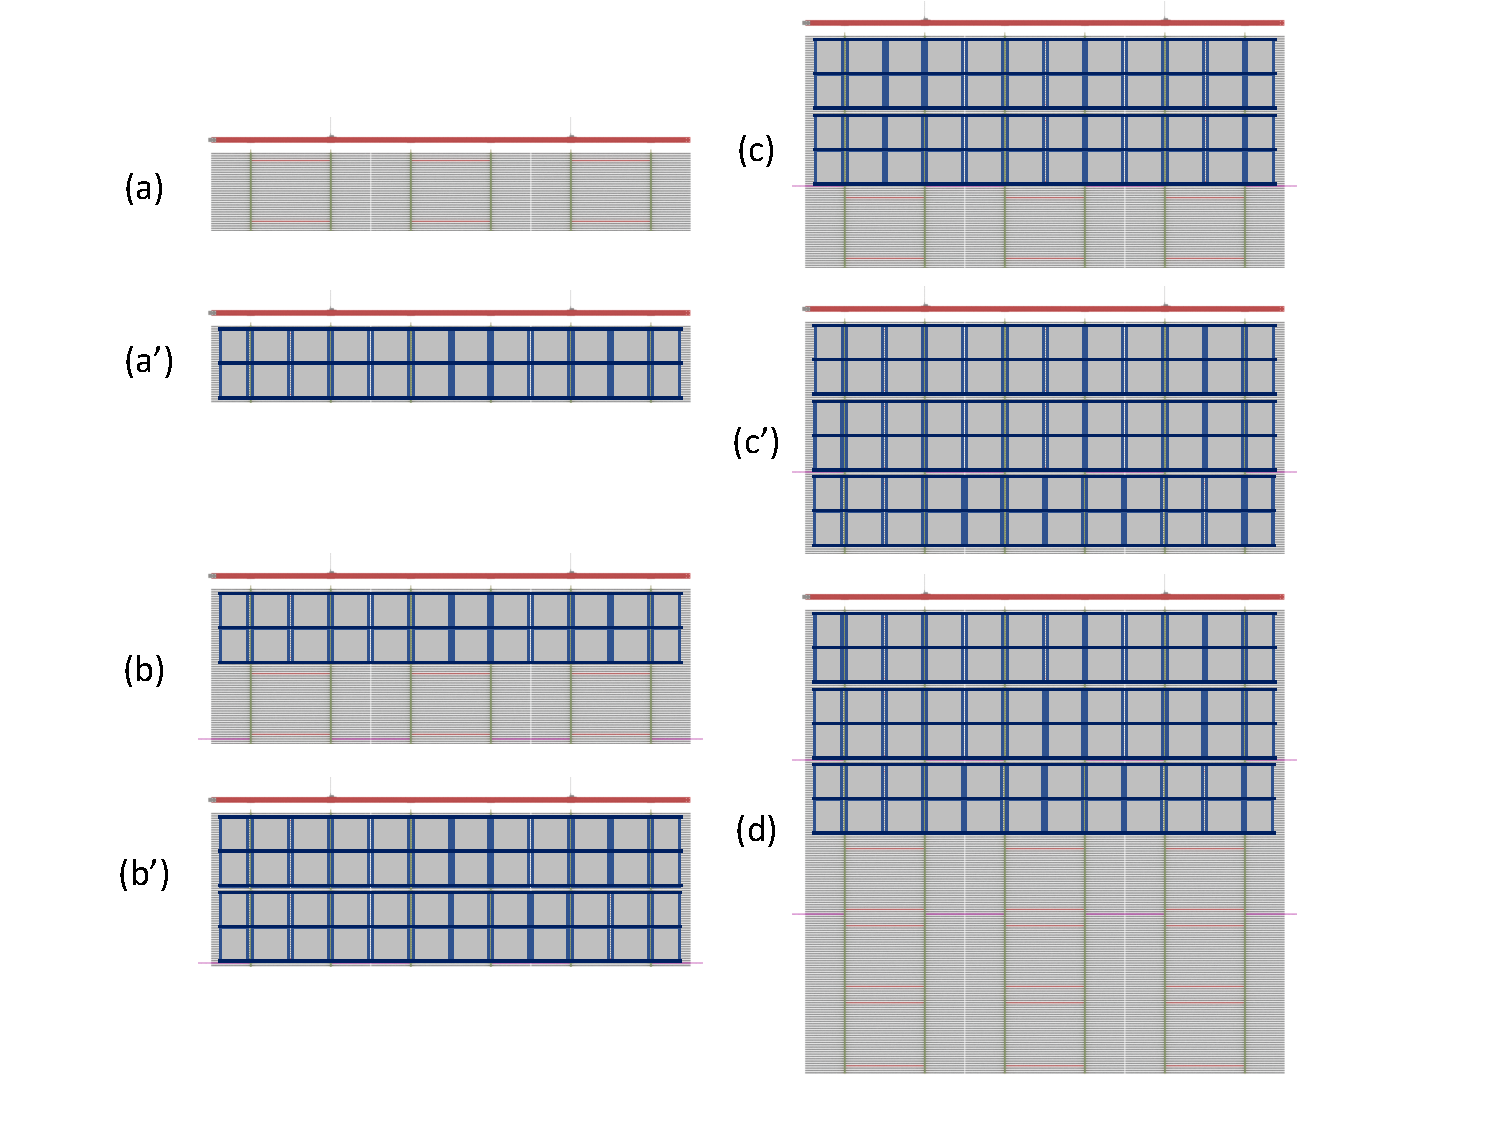
\includegraphics[width=0.9\textwidth]{DP_HVS_FC_super_module_reflector_installation_sequence_v2}
\end{dunefigure}

The entire \dword{hvs}, including \dword{fc}, cathode, \dword{gg}, and the \dword{pds} reflector/\dword{wls} 
panels are installed in the following sequence.
\begin{enumerate}
    \item Construct the \endwall super-module (with \num{90} degree bent corner profiles) at the end of the cryostat opposite the \dword{tco}.
    \item Mount  a U-shaped stainless steel cathode \endwall perimeter tube ($\sim$\SI{50}{\mm} diameter) to the bottom of the \endwall super-module.
    \item Install %This is then be followed by installation of 
    the two super-modules along the side wall immediately next to the \endwall module.  
    \item %These side wall super-modules have resistive sheath pre-inserted into each profile to 
    Make the electrical connections to the \endwall super-module.
    \item %Once the two side wall super-modules are completed, 
    Pull in the bottom of the \endwall super-module (with the cathode perimeter tube) %is pulled in 
    \SI{50}{\cm} from its free hanging position, align it to the side wall super-modules on each side wall, and anchor it to the temporary floor. 
    \item Electrically connect the \endwall super-module and side wall super-modules %are then electrically connected 
    using the pre-inserted resistive sheath.
    \item Assemble a cathode module %\SI{4}{\m} (W) $\times$ \SI{12}{\m} (L) is then assembled 
    in place at the bottom of the two side \dword{fc} modules immediately next to the \endwall super-module.
    \item Connect the stainless steel perimeter cathode tube already mounted on the \endwall super-module %is connected 
    to the corresponding cathode tubes on the side wall super-modules, and anchor it to the false floor to ensure the mechanical stability of the \endwall super-module until the entire \dword{fc} is constructed.
    \item Once the \dword{fc} and cathode are completely installed, remove the temporary floor under the %installed 
    cathode, % is removed, and the 
    and clean the membrane floor. % is cleaned.
    \item Place \dwords{gg} %Ground grids with extended legs are placed 
    under the cathode plane with their legs extended.
    \item Install the \dwords{pd} %The photon detectors that cover the for 
    under these \dwords{gg}. %corresponding area are installed.
    \item Remove the leg extensions of the \dwords{gg} and lower them %are lowered 
    to their nominal height. % by removing the leg extensions.
    \item Repeat steps \num{7} through \num{12} %\fixme{12?} %are repeated one more time 
    to install the cathode, \dword{gg}, and the \dwords{pd} for the installed \dword{fc} modules. %to cover two \SI{4}{\m} wide modules from the \endwall.
    \item Install the remaining %Two additional 
    side wall super-modules. % are constructed and electrically connected to the existing side wall super-modules via resistive sheaths.
    \item Repeat steps \num{7} through \num{12} %\fixme{12?} % are repeated three times to cover the \SI{12}{\m} width of the \dword{fc}.
    %\item Steps 7 - 13 are repeated 
    except for the last \SI{4}{\m} wide module of the side wall super-modules that connect to the \endwall super-module on the \dword{tco} end of the cryostat.
    \item Repeat steps \num{7} through \num{12} % are carried out 
    one last time.
    \item Remove the floor anchors for the two \endwall super-modules. % are removed.
\end{enumerate}

%\clearpage
%\section{Organization and Management}
%\label{sec:fddp-hv-org}

%%%%%%%%%%%%%%%%%%%%%%%%%%%%

%\subsection{Institutional Responsibilities - 1 page}
%\label{sec:fddp-hv-org-consortium}
%%%%%%%%%%%%%%%%%%%%%%%%%%%%
%\subsection{Risks}
%\label{sec:fddp-hv-org-risk-1pg}

%\fixme{Some text must accompany the table. The "ID" in the table refers to the ID in the Risk Register.}
%Most of t
%The items presented in Table~\ref{tab:dpHVrisks} apply to \dword{pddp} and the \dune \dword{dpmod}, and have been addressed by \dword{pdsp}, other than  
%items 10, 11, and 13 since they are specific to the 
%\dwords{detmodule}. None have caused significant problems during the commissioning and early operation of \dword{pdsp}, with the partial exception of 
%item 6. Current streams occurring at intervals of several hours and localized on one specific \dword{fc} module required a ramp down of the \dword{hv} for a few minutes from the nominal \SI{-187}{kV} to a lower value for \dword{pdsp} is unknown at the time of writing this section because the \dword{pddp} has not yet been in operation in \dword{lar}. 
%Item 6 requires an accurate analysis of collected muon data (this activity is in progress in \dword{pdsp}) 
%and the disentangling of space charge effects. 
%These risks still persist for the \dwords{detmodule},  
%given the much larger detector scale and the more complex underground installation environment.

%\begin{dunetable}
%[High Voltage System Risk Summary]
%{p{0.15\textwidth}p{0.75\textwidth}}
%{tab:dpHVrisks}
%{High Voltage System Risk Summary.}   
%Item & Risk \\ \toprowrule

%1 & Broken resistors on voltage divider boards \\ \colhline
%2 & Broken varistors on voltage divider board \\ \colhline
%3 & Cathode: Sharp corners at the voltage divider board connections\\ \colhline
%4 & Cathode: Truss connections to the field cage\\ \colhline
%5 & Angled \endwall super module installation\\ \colhline
%6 & Electric field uniformity is not adequate for muon momentum reconstruction \\ \colhline
%7 & Electric field is below specification during stable operations\\ \colhline
%8 & Damage to readout electronics in the event of discharge \\ \colhline
%9 & Detector components are damaged during shipment to the far site  \\ \colhline
%10 & Damages (scratches, bending) to aluminum profiles of Field Cage modules  \\ %\colhline
%11 & International funding level for DP HVC too low  \\ \colhline
%12 & Sole source for Kapton resistive surface; and may go out of production \\ \colhline
%13 & Free hanging frames can swing in the fluid flow  \\ \colhline
%14 & FRP/Polyethene/laminated Kapton component lifetime is less than expected  \\ \colhline
%15 & Underground installation is more labor intensive or slower than expected  \\ 
%\end{dunetable}

%\subsection{High-level Cost and Schedule - 2 pages}
%\label{sec:fddp-hv-org-cs}

%\fixme{Cost Summary Table goes in this section.}

%\fixme{Schedule Summary Table goes in this section.}

%\clearpage

\section{Design Validation and Verification Plan}
\label{sec:fddp-hv-verification}

Section \ref{sec:fddp-hv-protodune}  %\fixme{Section~\ref{sec:fddp-hv-protodune}?} 
describes the changes to the design relative to %with respect to the 
\dword{pddp}. These changes on the cathode design address the sudden release of the energy stored between the cathode plane and the \dword{gg}. The change mainly consists of replacing the continuous metallic structure used in \dword{pddp} with a segmented and resistive one. %\fixme{already said} 
%R\&D is in progress to adapt the solid experience accrued from the Single Phase detector CPA to the DP cathode plane design.

On the \dword{fc} side, the main changes are removing all insulating materials facing the cryostat wall as well as changing the assembly and installation procedure for the \SI{12}{\m}$\times$ \SI{12}{\m} super-modules. 
This procedure will be tested with mock-up modules in Ash River, which can be carried out independently of the planned electrical performance testing in \dword{protodune2}.   %\fixme{already said}
The electrical behavior of the cathode and \dword{fc} structure will be studied in a %\dword{spice} 
simulation to  confirm the design intention and identify weaknesses. %It will be validated in \dword{pddp} II, with a similar \dword{fc} design tested earlier in \dword{pdsp} II. \fixme{??}

Tests of the \dptargetdriftvoltneg \dword{hvps} %power supply 
and cryogenic \fdth are planned to be carried out in a dedicated cryostat at \dword{cern} (as for the \SI{-300}{kV} one) when the joint R\&D with Heinzinger can make them available following the description in Section~\ref{sec:fddp-hv-hvps-fdth}.


%%%%%%%%%%%%%%%%%%%%%%%%%%%%
\section{Interfaces }
\label{sec:fddp-hv-transport-interfaces}

%\fixme{This section covers mechanical interface to the cryostat, including the penetrations}
%\fixme{Interfaces Table goes in this section.}

Table~\ref{tab:hvs_interface_table} details the interface documents related to \dword{dp} \dword{hvs}. Some of the basic interfaces are summarized below. 

\fixme{In the table, is HVFT an official abbreviation? It is not in the common glossary.}

\begin{dunetable}
[\dual HV system interface documents]
{p{0.25\textwidth}p{0.5\textwidth}l}
{tab:hvs_interface_table}
{\dual \dword{hvs} interface documents.}

Interfacing System & Description & Linked Reference \\ \toprowrule
\dword{pds} & \dword{fc}, cathode, \dword{gg} and \dword{pds} \dword{pmt}, and reflector/\dword{wls} panel assemblies installation sequence, possibility of individual \dwords{gg} on the \dword{pmt} support structures  & \citedocdb{6799} \\ \colhline

\dword{crp} & HVFT penetration through \dword{crp}; installation sequence & \citedocdb{6754} \\ \colhline

Facility & cryogenic pipes locations; \dword{fc} suspension and \dword{hv} \fdth{} ports  & \citedocdb{6985} \\ \colhline

\dword{cisc} & \dword{hvps} control, monitoring, and interlock system; cameras & \citedocdb{6787} \\ \colhline

Calibration & calibration laser placement and \dword{fc} openings & \citedocdb{14005} \\

\end{dunetable}

\subsection{Internal Cryogenics System}
\label{sec:fddp-hv-intfc-to-cryogenic}

The interface with the cryogenics system involves coordinating placement of the cryogenic pipes. The locations of the \dword{gg} feet and the \dwords{pmt} must clear the cryogenic pipes and the membrane corrugations on the floor. 

\subsection{Cryostat}
\label{sec:fddp-hv-intfc-to-cryostat}

The cathode and \dword{fc} are suspended under the cryostat roof through special \fdth{}s. The \dword{hv} \fdth requires a port on the cryostat at a specific location.  The locations, sizes, heights, and load-bearing capabilities of these roof penetrations are being coordinated to allow detailed design of the \dword{hvs}.

%Each \dword{fc} module is suspended and raised by two ropes hung from the cryostat roof through the \dword{fc} suspension \fdth{}s, by winches as in \dword{pddp}.  

%Once an \dword{fc} module of the full height is completed for \dune \dword{dpmod}, it will be hung  from the cables attached to the final suspension hook and the  suspension \fdth is then fully sealed. 

%A possible improvement on the \dword{pddp} interface is to use remote-controlled electrical wrenches (as opposed to manual) to ensure synchronized lifting of the modules.

%%%%%%%%%%%%%%%%%%%%%%%%%%%%%%%%%
\subsection{Charge Readout Plane}
\label{sec:fddp-hv-intfc-to-crp}

The \dword{hv} and \dword{crp} systems are independently suspended and do not physically touch each other.  The relative vertical position between the top \dword{fc} profiles and the \dword{crp} affects the drift field uniformity near the \dword{crp}.  The \dword{crp}  dynamically follows the liquid surface whereas the height of the \dword{hvs} is fixed, so the maximum excursion of the \dword{crp}-liquid level must be controlled to avoid excess drift and extraction field distortion.

The \dword{hv} \fdth and extender structure goes through a corner of the \dword{crp}.  A special \dword{crp} module must be constructed to allow the \dword{hv} \fdth to be installed.


%%%%%%%%%%%%%%%%%%%%%%%%%%%%%%%%%
\subsection{Photon Detection System}
\label{sec:fddp-hv-intfc-to-pds}

%No direct hardware interface exists between the \dword{hv} and \dword{pd} systems. The cryostat penetrations and \fdth{}s for the two systems are completely independent, as are their control electronics. The only interfaces envisaged are effectively at the level of design requirements and include 

The cryostat penetrations and \fdth{}s for these two systems are completely independent, as are their control electronics. The suggested interfaces are effectively at the level of design requirements and installation coordination, and include

\begin{itemize}
    \item maintaining a safe minimum distance between the \dwords{pd} and the \dptargetdriftvoltneg cathode;
    \item defining a mutually agreed upon optical transparency of the cathode + \dword{gg} combination.  In general, a more open cathode and \dword{gg} will have a higher \efield on the cathode/\dword{gg} surfaces;
    \item  defining the \dword{pd} power dissipation limit (production of bubbles would compromise \dword{hv} stability); %The power dissipation depends on the final \dword{pd} density chosen, which is awaiting simulation results;
    %\item if the \dword{pds} wants to install reflector foils on the \dword{fc}, \dword{hvs} is to design a specific mounting feature for the reflector foils;
    \item agreement on the design of the reflector/\dword{wls} panel assemblies to be mounted on the inner walls of the \dword{fc}; 
    \item understanding of the effect on the \dword{fc} structure (weight, force from liquid flow);  
    \item developing an efficient installation plan; and
    \item installing individual \dwords{gg} on the \dword{pmt} supports (under discussion with the \dword{pds} consortium).
\end{itemize}


\subsection{Cryogenics Instrumentation and Slow Control}
\label{sec:fddp-hv-intfc-to-cisc}

The \dword{hvs} relies on \dword{cisc} to control the \dword{hvps} and monitor the supply and return currents from the \dword{fc} power return circuits.  An interlock of the \dword{hv} power supply with the liquid level will be implemented to prevent \dword{hv} discharge in gaseous argon.  A controlled shutdown of the \dword{hvps} with the opening of the cryostat pressure relief valve must also be implemented. A few strategically placed cryogenic cameras near key \dword{hvs} components would be very helpful.

\subsection{Calibration}
\label{sec:fddp-hv-intfc-to-cal}

The strong likelihood of non-negligible space charge distortion from positive ions in the \dword{dpmod} means calibration lasers are essential to provide accurate mapping of the drift field inside the \dword{tpc}.  The calibration laser beams must pass through the \dword{tpc}'s \dword{fc}.  Locations of the laser heads and their openings on the \dword{fc} must be coordinated.


\subsection{Technical Coordination}
\label{sec:fddp-hv-intfc-to-tc}

The shipping, storage, underground transportation, assembly, and installation of all \dword{hvs} components are coordinated with \dword{tc} and the \dword{jpo} (see Volume~\volnumbertc, \voltitletc).




%%%%%%%%%%%%%%%%%%%%%%%%%%%%%%%%%%%%%%%%%%%%%%%%%%%%%%%%%%%%%%%%%%%%
%\section{Installation, Integration and Commissioning}
%\label{sec:fddp-hv-install}
%\fixme{this is kind of mixed up with the next section -anne}

%%%%%%%%%%%%%%%%%%%%%%%%%%%%%%%%%%%%%%%%%%%%%%%%%%%%%%%%%%%%%%%%%%%%
\section{Organization and Management}
\label{sec:fddp-hv-org}
\fixme{Compare to SP HV org/mgmt section before finalizing. anne}
%%%%%%%%%%%%%%%%%%%%%%%%%%%%%%%%%%%
\subsection{HV Consortium Organization}
\label{sec:fddp-hv-org-consortium}

The \dword{hvs} consortium includes %has consolidated 
all the institutions participating in the design, construction, and assembly of the \dword{hv} systems for both \dword{pdsp}  and \dword{pddp}, 
%The consortium 
currently comprising several USA institutions and \dword{cern}, %presently 
the only non-USA participant. As it has been for \dword{protodune}, \dword{cern} is %heavily
strongly committed to taking on a significant role in terms of funding, personnel, 
 and providing infrastructure for R\&D and detector optimization. Moreover, \dword{cern} will be responsible for a significant fraction of subsystem deliverables; as such,  \dword{cern} is actively searching for additional European institutions to join the consortium. Table \ref{tab:instit} shows the list of institutions participating in the \dword{hvs} consortium.
 
 In the current \dword{hv} consortium organization, each institution naturally assumes the same responsibilities that it assumed for \dword{pdsp} and \dword{pddp}.

The consortium organizational structure includes a scientific lead from \dword{cern}, a technical lead from \dword{bnl}, and %, or as for the \dword{pddp}, 
a \dword{tdr} editor from the University of Texas at Arlington.  \dword{hvs} design and integration is presently led by \dword{cern}. 
The consortium is organized into working groups addressing design and  R\&D issues, as well as producing and installing the hardware.

\begin{itemize}
\item WG1. Design optimization for the \dword{sp} and \dword{dp} \dwords{detmodule}; assembly, system integration, detector simulation, and physics requirements for monitoring and calibrations. %Conveners: Jeff Nelson, Vic Guarino, Bo Yu
\item WG2. R\&D activities and %, R\&D 
facilities. %Conveners: Francesco Pietropaolo, Ting Miao
\item WG3. \dword{sp}-\dword{cpa}: Procuring resistive panels, frame strips, and electrical connections of planes; assembly, \dword{qc} at all stages, and shipping of these parts. %Convener: Stephen Magill
%\fixme{too many QC's. And confusing. Procurement, assembly, QC at all stages, and shipment of these parts? Anne - Done RKP}
%\fixme{Not sure where this came from - do you want detailed list of duties or should it just be the name of the group? - SRM; Simplified: FP}
\item WG4. \dword{dp} cathode and \dword{gg}:  procuring material; construction, assembly, shipping to South Dakota; % ITF, 
\dword{qa} and \dword{qc}.% Convener: Jae Yu
\item WG5. \dword{sp} \dword{topfc}, \dword{botfc}, and %top and 
\dword{ewfc} modules. %}bottom-\dword{fc} module, 
%\dword{sp}-\endwall modules, \dword{dp}-\dword{fc} modules: procurement of mechanical and electrical components, assembly and shipping to ITF. %Conveners: Thomas Kutter, Michael Wilking, Jeff Nelson, Jae Yu
%\fixme{ditto. Anne}
\item WG6. \dword{hv} supply and filtering, \dword{hv} power supply and cable procurement, R\&D tests, filtering and receptacle design and tests. %Conveners: Franco Sergiampietri, Sarah Lockwitz
\end{itemize}

%Merging of \dword{sp} and \dword{dp} activities is performed for the working groups where synergies have been identified: 
Taking advantage of identified synergies, some activities of the \dword{sp} and \dword{dp} working groups are merged: \dword{hv} \fdth{}s, voltage dividers, aluminum profiles, \dword{frp} I-beams, and assembly infrastructure.

\begin{dunetable}
[Participating institutes]
%{p{0.50\textwidth}p{0.15\textwidth}}
{ll}
{tab:instit}
{Institutes participating in the HVS consortium.}   
Institution & Country \\ \toprowrule%(Contact, E-mail) 

\dword{cern} & Switzerland \\ \colhline%(Francesco Pietropaolo; francesco.pietropaolo@cern.ch) 
Argonne National Lab& USA \\ \colhline%(Steve Magill; srm@anl.gov) 
Brookhaven National Lab& USA \\ \colhline%(Bo Yu; yubo@bnl.gov) 
University of California Berkley / LBNL & USA \\ \colhline%(Cheng Ju Lin; cjslin@lbl.gov)
 University of California Davis& USA \\ \colhline%(Emilja Pantic; pantic@ucdevis.edu) 
\dword{fnal} & USA \\ \colhline%(Sarah Lockwitz; lockwitz@fnal.gov) 
University of Houston & USA \\ \colhline%(Andrew Renshaw; arenshaw@central.uh.edu) 
Kansas State University& USA \\ \colhline%(Glenn Horton-Smith; gahs@ksu.edu)
Louisiana State University & USA \\ \colhline%(Thomas Kutter; kutter@phys.lsu.edu) 
%10 & South Dakota School of Mines and technology, USA (Juergen Reichenbacher; Juergen.Reichenbacher@sdsmt.edu) 
 SUNY Stony Brook & USA \\ \colhline%(Michael Wilking; michael.wilking@stonybrook.edu) 
 University of Texas Arlington & USA \\ \colhline%(Jaehoon Yu; jaehoonuy1@gmail.com) 
 Virginia Tech& USA \\ \colhline %(Jon Link; jmlink@vt.edu) 
College of William and Mary& USA \\ %(Jeff Nelson; jknels@wm.edu)  
\end{dunetable}

At present, the \dword{hv} consortium is gathering institutions to participate in the design, construction, and assembly of the \dword{hv} systems for both \dwords{spmod} and \dwords{dpmod}. 
The consortium is likely to expand in the near future. Discussions are underway with institutions, in particular from the EU, to balance USA participation with additional international partners.




%%%%%%%%%%%%%%%%%%%%%%%%%%%%%%%%%%
\subsection{Planning Assumptions}
\label{sec:fddp-hv-org-assmp}

The present baseline design for all elements of the \dword{hv} system for the \dune \dword{dpmod} follows the experience with \dword{pddp} as well as the \dword{pdsp} designs, including production and assembly.  

We %also 
assume that no major issues in the \dword{hv} system operation of \dword{pddp} will be encountered and that %therefore 
the basic \dword{hv} system concepts are sound.

However, some design modifications and optimizations have been implemented to take into account the %twice-as-long 
doubled drift distance, requiring \dword{hv} delivered to the cathode to increase from \SI{-300}{\kV} to \dptargetdriftvoltneg{} and the much higher energy stored in the cryostat as a result, %because of the applied \dword{hv}, 
and larger detector volume than \dword{pddp}.

Therefore, the \dword{dune} \dword{dp} \dword{hv} system distribution and the related cathode structure still require intense R\&D, given the unprecedented value of the required \dword{hv} (\dptargetdriftvoltneg) and the surface area covered by the cathode plane compared to \dword{pddp}. 
The related results could lead to revising design details such as the shape of the cathode elements and of the %\dword{gg} 
\dword{gg} structures, the distance from the cryostat walls, the distance between the cathode and the %\dword{gg} 
\dword{gg} protecting the \dwords{pd}, and resistive connections of the cathode modules. We must ensure that the \efield strength in the \dword{lar} remains everywhere below the critical value of  about \SI{30}{\kV/\cm}  and that the energy stored in the \dword{fc} is not released catastrophically to the cryostat membrane. 

%As in the \dword{spmod}, 
\dword{pddp} will be the testing ground where we come to understand and optimize detector element assembly, installation sequence, and integration, as well as requirements in human resources, space, tooling, and schedule. 

%%%%%%%%%%%%%%%%%%%%%%%%%%%%%%%%%%%

%\fixme{The editors at meeting of 2/13 suggest that the WBS section should be deleted in the TP. Accordingly, I have commented it out. RKP}

%%%%%%%%%%%%%%%%%%%%%%%%%%%%%%%%%%%
%\subsection{WBS and Responsibilities}
%\label{sec:fddp-hv-org-wbs}
%
%Consortium deliverables and related Working Breakdown Structure have also been derived from those identified for the ProtoDUNE detectors. As already mentioned before, responsibilities have been assigned to the institutions members of the Consortium, according to the experience gained with ProtoDUNE.
%
%\fixme{(Here: table to be extracted for the WBS excel file)}
%
%%%%%%%%%%%%%%%%%%%%%%%%%%%%%%%%%%

\subsection{Risks}
\label{sec:fddp-hv-org-risk}

%\fixme{new standard risks table for autogenerating latex as of 3/25. I will send email. Anne}

%the Risk Table 
Table~\ref{tab:risks:DP-FD-HV} %{tab:HVrisks} 
provides the risks items for the \dune \dword{dpmod} derived from those to be addressed in  %are the same in 
\dword{pddp}.  Some of these are common to \dword{pddp} and the \dword{dpmod}% (e.g., 1 and 2)
. Other  %ID's 
items (from 11 to 14)%(from 12 to 15)
, involving long term stability and funding, are specific to the \dword{fd} %Far Detector Underground Installation
\dwords{dpmod} construction and installation. 

Items common to \dword{pdsp}  have not caused significant problems during commissioning and early operation of \dword{pdsp}, with the partial exception of  %ID 
item 3%4
. For this specific issue, the operation of \dword{pddp} is essential because the \dword{hvs} layout is different, and the absolute voltage on the cathode is much higher. 
%ID 
Item 4 %5
will require an accurate analysis of collected muon data  %( a work-in-progress activity.) 
to disentangle space charge effects. 
These risks still persist for the \dwords{detmodule} %far detector case, 
given the much larger detector scale and the more complex underground installation environment.

\fixme{There should be a period at the end of the table title.}


% risk table values for subsystem DP-FD-HV
\begin{longtable}{p{0.18\textwidth}p{0.20\textwidth}p{0.32\textwidth}p{0.02\textwidth}p{0.02\textwidth}p{0.02\textwidth}} 
\caption{Risks for DP-FD-HV \fixmehl{ref \texttt{tab:risks:DP-FD-HV}}} \\
\rowcolor{dunesky}
ID & Risk & Mitigation & P & C & S  \\  \colhline
RT-DP-HV-01 & Broken resistors or varistors on voltage divider boards & Redundancy of resistors, varistors, and \dwords{hvdb}.  & L & L & L \\  \colhline
RT-DP-HV-02 & \efield uniformity is not adequate for muon momentum reconstruction & Regularly map out field using a laser calibration sysem. & L & L & L \\  \colhline
RT-DP-HV-03 & \efield is below specification during stable operations & Improve purity by more aggressive filtering. & M & M & L \\  \colhline
RT-DP-HV-04 & Space charge from positive ions distorting the \efield beyond expectation & Minimize insulators facing cryostat wall ground. & M & M & L \\  \colhline
RT-DP-HV-05 & Damage to \dword{ce} in event of discharge & Minimize the energy released in a short time using highly resistive connections. & L & L & L \\  \colhline
RT-DP-HV-06 & Energy stored in FC (in DP) is suddenly discharged & Delay energy discharge by connecting neighboring Al profiles with resistive sheaths.  & L & L & L \\  \colhline
RT-DP-HV-07 & Detector components are damaged during shipment to the far site & Make sufficient spares and increase the number of shipping boxes.  & L & L & L \\  \colhline
RT-DP-HV-08 & Damages (scratches, bending) to aluminum profiles of Field Cage modules & Make sufficient spares and increase the number of shipping boxes.  & L & L & L \\  \colhline
RT-DP-HV-09 & Bubbles from heat in PMTs or resistors cause HV discharge & A large area of cathode consists of high resistance rods, delaying the energy release.   & L & L & L \\  \colhline
RT-DP-HV-10 & Free hanging frames can swing in the fluid flow &  & L & L & L \\  \colhline
RT-DP-HV-11 & FRP/ Polyethene/ laminated Kapton component lifetime is less than expected &  & L & L & L \\  \colhline
RT-DP-HV-12 & Lack of collaboration effort on this HV system & Continue recruiting collaborators. & L & L & L \\  \colhline
RT-DP-HV-13 & International funding level for DP HVC too low & Employ cost saving measures and  recruit collaborators. & L & L & L \\  \colhline
RT-DP-HV-14 & Underground installation is more labor intensive or slower than expected & Increase labor contingency and refine labor cost estimates. Further improve installation procedure. & L & L & L \\  \colhline

\label{tab:risks:DP-FD-HV}
\end{longtable}
\begin{comment}

\begin{dunetable}
[DP HV system risk summary]
{p{0.02\textwidth}p{0.7\textwidth}p{0.095\textwidth}p{0.055\textwidth}}
{tab:HVrisks}
{High Voltage System Risk Summary.}   
ID & Risk  & Probability & Impact \\ \toprowrule

1 & Broken resistors on voltage divider boards & L & L \\ \colhline
2 & Broken varistors on voltage divider board & L & L \\ \colhline
3 & Electric field uniformity is not adequate for muon momentum reconstruction & M & L \\ \colhline
4 & Electric field is below specification during stable operation & M & L \\ \colhline
5 & Space charge from positive ions distorting the E field beyond expectation & M & L \\ \colhline
6 & Damage to \dword{ce} in event of discharge & L & L \\ \colhline
7 & Energy stored in \dword{fc} (in DP) is suddenly discharged.   & L & M \\ \colhline
8 & Detector components are damaged during shipment to the far site  & L & L \\ \colhline
9 & Damage (scratches, bending) to aluminum profiles of Field Cage modules  & L & L \\ \colhline
10 & Bubbles from heat in PMTs or resistors cause HV discharge  & L & M  \\ \colhline
11 & Free hanging frames can swing in the fluid flow  & L & L  \\ \colhline
12 & \dword{frp}/Polyethene/laminated Kapton component lifetime is less than expected  & L & L  \\ \colhline
13 & Lack of collaboration effort on this HV system  & M & M  \\ \colhline
14 & International funding level for DP HVC too low  & M & M  \\ \colhline
15 & Underground installation is more labor intensive or slower than expected  & L & L  \\ 
\end{dunetable}


%%%%%%%%%%%%%%%%%%%%%%%%%%%%%%%%%%%%%%%%
\subsection{High-level Cost and Schedule}
\label{sec:fddp-hv-org-cs}

%\fixme{new standard cost table will be coming in early April - for autogenerating latex. Anne}

%\fixme{Table~\ref{tab:dp-hv-sched} is a standard table template for the TDR schedules.  It contains overall FD dates from Eric James as of March 2019 (orange) that are held in macros in the common/defs.tex file so that the TDR team can change them if needed. Please do not edit these lines! Please add your milestone dates to fit in with the overall FD schedule.  Anne}

% If you want to get started quickly, find the new macros at the end of this file.

A first high-level summary of the cost estimate for the \dword{hv} system of one \dune \dword{dpmod} was obtained by extrapolating from the as-realized \dword{pddp} costs and labor, except for the cathode, which was introduced as a new concept and for which estimation is more uncertain. Moreover, these estimates do not include any projected cost savings that would be realized by producing many units at each production site. %Given the small numbers of each unit required for the \dword{pddp} the assembly sites were still climbing the learning curve; this could give substantial savings. 
However, substantial savings from higher-volume production is still possible. For \dword{pddp}, the assembly sites produced only small numbers of each unit, which left personnel on the learning curve. Table \ref{tab:HVcostsumm} shows the \dword{dp} \dword{hvs} cost summary.

\begin{dunetable}
[\dual HV system cost summary]
{p{0.5\textwidth}p{0.2\textwidth}p{0.2\textwidth}}
{tab:HVcostsumm}
{\dual High Voltage System Cost Summary. (TO BE COMPLETED)}   
Cost Item & M\&S (k\$ US) & Labor Hours \\ \toprowrule

Project Management &     &             \\ \colhline
Physics and Simulations &     &             \\ \colhline

\rowcolor{dunepeach} Design, Engineering and R\&D &  &     \\ \colhline
 \rowcolor{dunepeach} Production Setup &  &     \\ \colhline
 Cathode and ground grid  &     &             \\ \colhline
 \dword{fc} submodule &     &             \\ \colhline 
 HV feedthrough cold test &     &             \\ \colhline
 \rowcolor{dunepeach} Production &  &     \\ \colhline
 Cathode  &     &             \\ \colhline
 Ground grid &     &             \\ \colhline 
 \dword{fc} components &     &             \\ \colhline
 \dword{hvdb} &     &             \\ \colhline
 \dword{fc} submodules &     &             \\ \colhline
 \dword{hv} components &     &             \\ \colhline
\rowcolor{dunepeach} DUNE FD Integration \& Installation  &  &     \\ %\colhline
%\dword{pmt} Testing at \dword{ctsf} &     &             \\ \colhline
%\dword{wls} Production &     &             \\ \colhline
%\dword{wls} Testing &     &             \\ \colhline

%Signal/Optical Flanges Installation &     &             \\ \colhline
%\dword{pmt} Installation &     &             \\ \colhline
%\dword{pmt} Cabling and Optical Fibers to Feedthrough  &     &             \\ \colhline
%Cabling from Feedthrough to Splitter  &     &             \\ \colhline
%Cabling from Splitter to \dword{hv} Power Supply &     &             \\ \colhline
%Cabling from Splitter to \dword{utca} \dword{fe} Electronics &     &             \\ \colhline
%Light Electronic Rack Installation &     &             \\ \colhline
%Installation Tests &     &             \\ \colhline
%Commissioning &     &             \\ \colhline

\end{dunetable}
\end{comment}

Table \ref{tab:dp-hv-sched} shows the tentative  \dword{dp} \dword{hvs} schedule, assuming the  \dword{dpmod} technology is selected for the second \dword{dune} \dword{fd} module.

\begin{dunetable}
[\dual HV system schedule and milestones]
{p{0.65\textwidth}p{0.25\textwidth}}
{tab:dp-hv-sched}
{\dword{hvs} Consortium Schedule (\dword{dp}).}   
Milestone & Date (Month YYYY)   \\ \toprowrule
Technology Decision Dates & March 2020   \\ \colhline
Final Design Review Dates & Sept. 2020   \\ \colhline
Start of module 0 component production for ProtoDUNE-II & March 2021 \\ \colhline
\rowcolor{dunepeach} Start of \dword{pdsp}-II installation& \startpduneiispinstall      \\ \colhline
End of module 0 component production for ProtoDUNE-II & September 2021\\ \colhline
\rowcolor{dunepeach} Start of \dword{pddp}-II installation& \startpduneiidpinstall      \\ \colhline
\rowcolor{dunepeach}South Dakota Logistics Warehouse available& \sdlwavailable      \\ \colhline
Delivery of the \dptargetdriftvoltneg \dword{hvps} &  April 2022 \\ \colhline
\dword{prr} dates & September 2022\\ \colhline
Start of \dword{fc} production  &  September 2022 \\ \colhline
Start of \dword{hvdb} production  &  September 2022 \\ \colhline
\rowcolor{dunepeach}Beneficial occupancy of cavern 1 and \dword{cuc}& \cucbenocc      \\ \colhline
Start of cathode production  &  January 2023\\ \colhline
Start of HVPS, \fdth \& HV extender production  &     March 2023 \\ \colhline
\rowcolor{dunepeach} \dword{cuc} counting room accessible& \accesscuccountrm      \\ \colhline
Start of ground grid production  & May 2023\\ \colhline
\rowcolor{dunepeach}Top of \dword{detmodule} \#1 cryostat accessible& \accesstopfirstcryo      \\ \colhline
\rowcolor{dunepeach}Start of \dword{detmodule} \#1 TPC installation& \startfirsttpcinstall      \\ \colhline
End of \dword{hvps}, \fdth \& HV extender production  & January 2025     \\ \colhline
\rowcolor{dunepeach}Top of \dword{detmodule} \#2 accessible& \accesstopsecondcryo      \\ \colhline
End of \dword{fc} production  & March 2025\\ \colhline
End of \dword{hvdb} production  & March 2025 \\ \colhline
End of cathode production  & May 2025\\ \colhline
End of ground grid production  & May 2025\\ \colhline
\rowcolor{dunepeach}End of \dword{detmodule} \#1 TPC installation& \firsttpcinstallend      \\ \colhline
 \rowcolor{dunepeach}Start of \dword{detmodule} \#2 TPC installation& \startsecondtpcinstall      \\ \colhline
\rowcolor{dunepeach}End of \dword{detmodule} \#2 TPC installation& \secondtpcinstallend      \\ \colhline
\end{dunetable}




%\begin{dunetable}
%[\dword{hv} system materials costs]
%end{dunetable}
%\begin{dunetable}
%[DP High Voltage System Cost Summary]
%{p{0.7\textwidth}p{0.2\textwidth}}
%{tab:HVcostsumm}
%{High Voltage System Cost Summary}   
%Item & Core Cost (k\$ US) \\ \toprowrule

%Design, Engineering, and R\&D    & \num{0} \\ \colhline
%Physics \& Simulations           & \num{0} \\ \colhline
%Cathode and ground grid production setup  & \num{0} \\ \colhline
%\dword{fc} sub-module production setup  & \num{0} \\ \colhline
%HV feedthrough cold test setup   & \num{0} \\ \colhline
%Cathode production               & \num{0} \\ \colhline
%Ground grid production           & \num{0} \\ \colhline
%\dword{fc} component production         & \num{0} \\ \colhline
%\dword{hvdb} production         & \num{0} \\ \colhline
%\dword{fc} sub-module production         & \num{0} \\ \colhline
%HV component production         & \num{0} \\ \colhline
%Shipping \& Integration          & \num{0} \\ \colhline
%Installation                     & \num{0} \\ \colhline \colhline
%Total DP HV System (DP-HV)       & \num{0} \\
%\end{dunetable}

%\fixme{(this is to be extracted from the Cost excel file)}

%\begin{dunetable}
%[\dword{hv} System R\&D Program and Milestones to Lead to CD-2 Approval (THIS TABLE is to be UPDATED in Draft 2)]
%{p{0.07\linewidth}p{0.55\linewidth}p{0.10\linewidth}p{0.10\linewidth}p{0.10\linewidth}}
%{tab:HVschedule}
%{DRAFT- \dword{hv} system R\&D program and milestones.}   
%WBS&Task Name&Start&Finish \\ \toprowrule
%1.5&   CD-2 DOE Review&10/04/19&10/04/19 \\
%7& \dword{hv} System& & \\
%7.1& Finalize \dual \dword{fc} design&06/27/18&11/30/19 \\
%7.2& Finalize \dual cathode design&06/27/18&11/30/19 \\
%7.3& Finalize R\&D for 600 kV \dword{hv} \fdth and PS &01/01/18&02/28/19 \\
%7.4& Run \dword{dp} \dword{hv} design integration test &02/18/19&02/28/20 \\
%7.5& \dword{hv} TDR - Submit for internal review&03/29/19&03/29/19 \\
%7.6&\dword{fc} Procurement&  07/08/23& 05/03/24\\
%7.7& Cathode and Ground plane Procurement& 07/08/23& 03/04/24\\
%7.8& HV distribition procurements (including Voltage dividers)& 09/06/23& 11/29/24\\
%7.9& Production readiness reviews& 01/02/24& 01/07/24\\
%7.10& Cryostat ready for TPC installation& 08/01/24& 08/01/24 \\
%7.11& Cathode and Ground plane assembly& 05/03/24& 12/29/24\\
%7.12&\dword{fc} Assembly and installation &08/01/24& 02/03/25\\
%7.13& Cathode and Ground plane installation &08/01/24& 02/03/25\\
%\end{dunetable}
%\fixme{(to do: Schedule)}

%%%%%%%%%%%%%%%%%%%%%%%%%%%%%%%%%%%%%%%%%%%%%%%%%%%%%%%%%%%%%%%%%%%%

\section{Appendix - Alternatives}

%\subsection{Optical Reflectors on \dword{fc} FRP Frames}

%The \dual \dword{pds} has expressed interest in adding \dword{wls} coated reflector foils on the \dword{fc} inner surfaces to increase light collection efficiency for the upper portion of the \dword{tpc}.  

%The reflector foils on their own are very thin and fragile, with different CTE than the rest of the \dword{fc} structure. Unsupported large sheets, therefore, should not be mounted directly onto the \dword{fc}.  However, laminating the reflector foil over a G10/FR4 sheet creates a panel that could be easily attached over the \dword{fc} FRP I-beams.  Since the G10 sheet has a lower CTE than the stainless steel \dword{fc} cross bars, some sliding motion on the mounting fixture is envisioned.

%If the area coverage required is less than \num{50}~\%, the reflector foils may be cut into strips and  installed onto each of the \dword{fc} profiles without interfering with the liquid flow.

%The effect of the reflector panels, if their coverage area is large, on the \dword{lar} flow pattern and the force exerted on the panels must be studied before this option is chosen.

\subsection{Calibration Laser Penetrations}

%Despite being in an underground environment, the \dual detector should have non-neglegible space charge distortion due to the ion feedback from the multiplication of $^{39}$Ar ionizations through the \dwords{lem}. The liquid argon convective flow will make the space charge density distribution difficult to model accurately. Therefore, using UV laser beams is highly desirable to calibrate the charge signal based on the measured field distortions throughout the \dword{tpc} volume.
Despite its underground environment, the \dword{dune} \dword{dpmod} is likely to have non-neglegible space charge distortion due to the ion feedback from the multiplication of $^{39}$Ar ionizations through the \dwords{lem}. The \dword{lar} convective flow will make the space charge density distribution difficult to model accurately. Therefore, using UV laser beams is highly desirable to calibrate the charge signal based on the measured field distortions throughout the \dword{tpc} volume.

We have designed a \SI{15}{\cm} offset between the \dword{fc} and the edges of the \dword{crp}, so %we may be able 
it may be possible to place laser heads through this gap to scan the \dword{tpc} active volume. Obviously, the stainless steel \dword{fc} support I-beam is in the way, but it should be fairly straightforward to make openings through the I-beam 
%\fixme{Which I-beam is this, the stainless steel I-beam the FC hangs from? if the reflective foils are to be now in the base design the interference with the laser should also be meintioned.}
to allow a $\sim\,$\SI{10}{\cm} \dword{od} object through. This feature will be designed and developed if the calibration consortium decides to implement a laser system.  Naturally, %the penetrations for the lasers would need to be planned in 
the cryostat design % if such a system is likely.
would need to incorporate the penetrations for the lasers.

\subsection{Individual Ground Grids on PDS PMTs}

 Installing an individual \dword{gg} for each \dword{pmt} in place of the ground grid table structure is under consideration in collaboration with the \dword{pd} consortium. Because the individual \dword{gg} cages would potentially have thinner wires and be closer to the \dword{pmt} windows, thus generating  smaller shadows, they should increase light transparency to the \dwords{pmt}.

The  \dword{hv} consortium will study the  operational feasibility of the design % in terms of operation in the \dune \dual 
under \dword{dune} \dword{dpmod} conditions.  Engineering teams from both consortia will jointly develop the design of the individual grids, the %production of the grids will be done by 
\dword{hv} consortium would produce them, and the \dword{pd} consortium would install them  %The grids will be installed %at the \dword{itf} Anne removed
%by \dual . The \dwords{pmt} will be installed 
with their individual grid cages. % by \dual \dword{pd} consortium. 
